\documentclass[a4paper,11 pt]{report}

\usepackage[utf8]{inputenc}
%\usepackage[T1]{fontenc}
%\usepackage{babel}
\usepackage{graphicx}

% sudo apt-get install texlive
\usepackage[font=small,format=plain,labelfont=bf,up,textfont=it,up]{caption}

\usepackage{amsmath}
\usepackage{mathrsfs} %brukt for krølle-L : laplace

\usepackage{listings} %for c++ kode
\lstset{language=c++}

%Kanskje dette er naudsynt? For metapost:
%\DeclareGraphicsRule{*}{mps}{*}{}


\author{Per R. Leikanger}
                             
\title{Project}
\date{\today}     

%\usepackage{natbib}    Kva er dette? Er med i rapport 3002.

\begin{document}   

\maketitle

%TODO 
Mealey vs More state maschine model of spiking Artificial Neural Network. A comparison.
% Er dette en mulig tittel?


Når det gjelder skriving, så er det veldig effektivt med uttrykk som "the rationale behind the choise of letters $n$,$s$, and $a$ is explained in chapter 3."
Bruk dette! 
Frampeik, med litt mystikk som impliserer at eg veit meir enn leser. (Hugs norsk fra grunnskulen: frampeik er bra!)
I tillegg til at det impliserer at eg har tenkt mykje over saken, så syr det teksten bedre sammen!


\chapter{Om oppgaveteksten:}
Les meir grundig det som står på toppen. Den punktinndelte oppgava på bunnen gir følgende notater:

Eit poeng: "(NB: Hold deg innenfor oppgaven,du kan ikke regne med å få
kreditt for arbeid som går på siden av oppgavens uttalte fokus)."
------> Skriv kvifor eg har implementert simuleringa så nøyaktig. Begrunn dette, for å få uttelling for det i karrakteren. 

Hold også eit auge med skrivet eg fekk fra Øyvind S.: Korleis gjennomføre prosjekt. Spesiellt i forhold til innledning er dette viktig!
	\section{Pkt. 1}
Oppgaveteksten seier: "Gi en oversikt over eksisterende modeller for ANN som representerer både fyringsrate og -tidspunkt. 
Legg spesielt vekt på forhold som kan knyttes til stabilitet under læring og/eller tilbakekobling ("recurrent ANN")."

Første setninga kan tolkes, men eg trur tolkininga som går på at det er en modell som representerer begge er mest rett (BÅDE). 
Trur ikkje det er nokon modell som gjør dette. Kan skrive dette, så skrive om modeller som representerer fyringsrate ELLER -tidspunkt. (fANN, SANN).


	\section{Pkt. 2}
"Beskriv det nye konseptet, og påpek hvordan dette skiller seg kvalitativt fra tidligere kjendte metoder."

Tolkning: tidligere kjendte metoder - tidligare modeller som representerer tidspunkt for fyring. Bare SANN!

Ellers er dette punktet rett--fram.

	\section{Pkt. 3}
"Foreta en sammenlikning av det nye konseptet og konkurrerende metoder. Evalueringen kan baseres på et antall konkrete scenarier(mhp. inngangsdata osv.)."

Tolkning:
Konkurerende metoder er andre metoder som også representerer tidspunkt for spikes. Dette er bare SANN (kanskje ta med ulike implementasjonsmetoder av SANN? Timedriven/eventdriven?)
Eg tenker at eg ikkje får tid til å gjøre en omfattende sammenligning av effektivitet, så sammenligner med bakgrunn i implementasjon. 

Sammenligne litt for effektivitet (for ulike oppsett).

Sammenligne tematisk? Skrive at eine er Moore, andre Mealy auromata?


\tableofcontents

\newpage

\newpage

% KAPTITTEL : Introduction
%TODO Må skrives: sett av 0.7 dag til dette.

%Todo Skriv kvifor eg 'cite' kapittel til de ulike bøkene. Bøkene er ofte så store at uten dette blir referansene memingsløs..




%
% 	- Utvida innholdsfortegnelse.
% 	- Skrive at eg har, og vise til kor eg har    ->  svart på de ulike aspektene ved oppgaveteksten.
% 	- Skrive eksplisitt om oppgaveteksten.
% 	- 
% 	- 

\section{Introduction}
Artificial Neural Networks(ANN) is often used for artificial intelligence or other computer algorithms that require learning.
Traditionally, a frequently based neuron is used to model each node.
In this scheme, each node of the ANN gives an output based on the present input.
This model use a continuous ``activation function'' to compute the output of a node.

Lately, there has been an increasing awareness among neuroscientists that the relative spike time of two neurons is important for the synaptic plasticity in the connecting synapse.
This has led to the developent of what is referred to as ``the third generation ANN''.
Spiking Artificial Neural Networks(SANN) uses a simlified matematical model of the biological neuron to give its behaviour. %the behaviour of the biological neuron. 
%Spiking Artificial Neural Networks(SANN) use a direct simulation of a simlified matematical model of the neuron to give the behaviour of the biological neuron.
The most common used model is the ``Leaky integrate--and--fire''(LIF) neuron\cite{Maass97networksof}.
% % % 
As the value of a LIF neuron is time--variant, the value of the node has to be simulated. 
This involves an updating of the value, either every time the value is used or every time iteration of the ANN.
As a direct simulation of a time variant signal is computationally demanding, a time--invariant signal is preferable.

New equations for modelling the LIF neuron has been developed based on mathematics from electronics and cybernetics.
An equation for the value of the neuron was turned around, and can be used for calculating the time when the value reaches a certain threshold.
If this threshold is the firing threshold of the neuron, this equation gives a calculation of the interspike period of the neuron.

In this report, a novel model for ANN with the capability to calculate the spike time is introduced.
A simple simulation is performed, and the result is compared to that of node of a SANN node.

\emph{Chapter 1} $\;$ introduces relevant background information. 
	First, a short review of the history of ANN is introduced. This gives an introduction to the development of ANN. After this, important aspects of the biological neuron is introduced, with a focus on its signal processing mechanisms.

In \emph{Chapter 2} $\;$ the new model is evolved. The modelling chapter starts from scratch, with the depolarization equation for the value. From this it eventually presents the mathematics behind the new ANN model.

\emph{Chapter 3} $\;$ introduces the design and implementation of the two models used. 
	The first section is about the general design that will be common to both implementations. Elements that are important for execution and  theoretical and experimental comparison will be introduced in this section.
	Following the general design, the design and implementation details will be introduced.

Finally \emph{Chapter 4} $\;$ presents the comparions and discussion of the results.
	The chapter will start with a section containing a theoretical comparison between the two designs.
	The experimental results are presented and compared in the next section.
	For the remainder of the chapter, a final discussion and concluding remarks are presented.





%Korleis skrive rapport:
%
%State the problem addressed in the report and explain why the problem is significant. Depending on the complexity of both, this may be done in one or two sentences.
%
%Describe the purpose or goal(s) of the report--what you were asked to accomplish.
%
%Provide general background information the reader needs to know to understand the report, such as the methods and theories used to gather the information.
%
%Explain the scope of the report's contents, including what is covered and, if necessary, what is not covered. For example, your report may include findings made during an investigation but not recommendations about how to respond to those findings.





% XXX Følgende er kjempeviktig å ha med:
% In this report the convention used by Rolls and Treves in ``Neural Networks and Brain Functions'' will be used. 
% For any transmission through a synapse between neuron $j$ and neuron $i$, we define the synaptic strength $w_{ij}$.  % TODO Skriv heller: "..through a synapse FROM neuron $j$ TO neuron $i$, we .."
% Note that the first subscript refers to the recieving neuron and the last subscript to the presynaptic neuron (the signalling neuron) \cite{TrevesNeuralNetworks}.
% This convention will be used in this text. 
% % XXX XXX XXX  (bra skrevet er det og)
 


%%%%%%%%%%55
% Skriv litt om korleis denne rapporten kan brukes:
% Denne rapporten er en rapport på eit ommfattende arbeid, med elementer som har blitt jobbet med i oppmot 2 år.
% Dette gjør at det kanskje blir litt mykje å lese den "perm til perm", men eit forsøk har blitt gjort for å komprimere stoffet til under hundre sider med tekst.
% 
% Siden mykje av de diskuterte mekanismane er kompleks, funker ikkje uml, men ting må forkleres. Dette har blitt forsøkt.
% Mykje innhold gjør likevel at det kanskje kan bli litt mykje å bite over for en leser, og rapporten er kanskej best som eit opopslagsverk. 
% (så skriv utvida innholdsfotegnelse, med fokus på også element som kan være nye, som sceduler, KANN, osv.)
% %%%%%%%%%%55



%TODO NEVN action potential i innledning! XXX VIKTIG!




%(tidligere) KLADD:
%Recently, there have been a strong focus on the timing of spikes. There are two reasons behind this.
%The first is connected to synaptic plasticity. 
%In 1987, Gustavsen et. al. found that synaptic plasticity could vary as a function of the postsyn
%Synaptic plasticity can be divided in two groups, Long Term Potentiation (LTP) causing an a lasting increase in the synaptic weight and Long Term Depression (LTD) causing a lasting decrease in the synaptic weight.
%Gustavsen et. al found in 1987 that the synaptic plasticity vas a function of the postsynaptic depolarization at the time of transmission. 
%The synaptic plasticity varied from a strong LTP to a strong LTD as a result from a single transmission\cite{Gustafsson03011987}.
%%Dette ble også overført til ANN

%We can say that, statistically there is a correlation between the presynaptic depolarization after a synaptic transmission, and the relative timing of the postsynaptic action potential. %ELLER NOKE: RYDD OPP XXX XXX
%If we view this statistically, we can say that the timing of the presynaptic action potential (``firing'') in relation to the postsynaptic firing is a direct consequence of the postsynaptic potential at the time of transmission.
%Based on this analysis alone, we can say that the relative timing of the pre-- and post-- synaptic firing is fundamental for the size and direction of the synaptic plasticity.
%% XXX KVIFOR tidavhengig? XXX : There are also hypothesis about a retrograde signalling mechanism in the neuron that gives the same effect
%This recieved the name ``Spike Time Dependent Plasticity''(STDP).








%TODO Skriv at eg kaller implementasjonen for AuronSim, og dette navnet vil opptre under mange av kurvene i rapporten.


%todo todo todo Skriv kvifor eg har så mykje neuro-info: dette kan sees på son en del av utviklingsprosessen: det å lære om neuronet er viktig for å skrive en simulator av dette..

% Skrive at denne teksten er laget som resultat av arbeidet mitt.
% I mange tilfeller der det ikkje er referanser er dette fordi eg ikkje har basert denne delen av arbeidet på andres arbeid, men utvikla det selv. 
% 	Dette gjelder spesielt for SANN modellen min, siden eg begynte dette arbeidet før eg i det heile tatt viste at det fantes noko som var kalla SANN. Mangler på referanser er dermed selvfoklart. 
% 	Eg har i desse tilfeller prøvd å få med store deler av utviklingsprosessen.
%
% For KANN har eg enda ikkje funnet andre modeller basert på desse ligningene, og er fortsatt av den tro at dette er nytt arbeid.
% 	For KANN har eg difor alltid vist utviklignsprosessen for både modellen og impelmentasjonen. Dette ble mye tekst, men dette er eit resultat av mangler på kilder å henvise til.
%
% Før eg kan begynne å snakke om SANN modellen eller KANN modellen trenger eg å etablere eit felles utgangspunkt for forfatteren og leseren. 
% 	Dette er forsøkt gjordt ved å ha en grundig gjennomgang av ANN og det biologiske systemet,tidlig i teksten(i kap. 1). Supplerende informasjon og informasjon som faller utenfor oppgaven er plassert i appendix, og er også egenprodusert.
% 	
% Kap. 2 er forbeholdt modellering av neuronet, og for innføring i bakgrunnsmatematikken som ligger bak den nye modellen.
% 	Det er godt mulig at resultatene fra dette kapittelet også kan være til bruk for neuralscience, da det gjør eit forsøk på å etablere bedre fremgangsmåter for "aktivitetsvariabler" for neuronet. 
% 	Den gjeldende aktivitetsvariabelen for neuron er basert på fyringsraten til neuronet, noko som ikkje er særlig intuitivt med tanke på "instataneouis firing rate". Den nye modellen opner for umiddelbare aktivitetsvariabler.
%
% 	I de to første kapittel er mesteparten av bakgrunnsinformsjonen presentert, så mesteparten av 'citations' vil finnes her. Seinere kapittel vil inneha ferre 'citations', da dette i all hovedsak er basert på eget arbeid.
% 		XXX Kanskje dette ikkje stemmer for Kap 3? Veit ikkje enda, siden det ikkje er skrevet. Trur ikkje det..
%
% Kap. 3 Omhandler design og implementasjon av de ulike modellene. 
% 	Section {ref:design} handler om den generelle strukturen for implementasjonane. Her beskrives flere metoder for å gjøre implementasjonene mest mulig sammenlignbar for denne oppgaven.
% 		Resultat presentert i kapittel 1 vil være viktig i dette kapittelet, siden implementasjonene er prøvd å gjøres lik det biologiske systemet. 
% 		Den modulære oppbyggingen til det kunstige neuronet (auronet) er beskrevet og  vil være gjeldende for begge modellene.
% 		Element som object design og metoder for effektivisering vil bli presentert.
% 		I tillegg vil en "to my knowledge" ny modell for tid bli presentert. Denne modellen er viktig for begge modellene, siden den gir oss mulighet for å ha simulert asynkronitet for nodene i neuralnettet.
% 		Logg. pCalculationTaskQue, pWorkTaskQue?, ...
% 	Section {ref:SANN-imp} handler om design og implementasjon av SANN
% 		Dette kapittelet går gjennom mekanismene som ligger bak simulering av mitt SANN. Dette kapittelet lener seg sterkt på element presentert i kapittel 1 og litt fra kap. 2.
% 		Modellen er egenprodusert, selv om den tidligere har blitt etablert (REFER til når/kor/kven). Dette dobbeltarbeidet er en konsekvens av manglende kunnskap for kildesøk når eg studerte neuro.
% 		Section {SANN-imp} avaluttes med en utskrift (plot) laget ved en kjøring av SANN simulatoren.
% 	Section {ref:KANN-imp}
%  		Dette kap. begynner med å beskrive konsept som må behandles ulikt fra det som er presentert i section {SANN-imp}. 
% 		Siden modellene er basert på heilt fremgangsmåter for å simulere eit LIF neuron, begynner forskjellene allerede ved aktivitetsvariabelen.
% 			For SANN er artivitetsvariabelen en etterligning av det biologiske neuronets aktivitetsvariabel, det elektriske potensialet over membranen. 
% 			For KANN er aktivitetsvariabel basert på resultat fra kap. 2, som er, så vidt eg veit, en heilt ny måte å modellere neuronets aktivitet på.
% 		Dette skaper også ulikheter i korleis aktivitet propagerer gjennom systemet. Mykje av det resterende i section{KANN-imp} er brukt på dette.
% 		Mot slutten diskuteres metoder for å gjøre KN kompatibel med SN, spesielt i retninga KN->SN. 
% 		Section{KANN-imp} avsluttes med en diskurs om når Kappa bør propagere videre til neste noder. Dette er eit viktig element og (BØR) dekkes grundig. TODO Dekk grundig!
% 		%KANSKJE lag eit plott som ligner på plottet i {SANN-imp} og skriv at kapittel avsluttes med samme som {SANN-imp}.
% Kap 4 er avsatt sammenligning og resultat av prosjektet. TODO Skriv dette etter at eg har skrevet Kap 4 XXX
%
%
%
%
% 	Aspekter ved oppgaven / kor er det besvart?
% 		Sammenligning: skriv at eg desverre ikkje fekk tid å sammenligne effektivitet, så denne tolkningen av oppgaven må vente til senere.
%
%
%
%





















% 	- 
% 	- 
% OPPSETT:
% 	- Oppgaveteksten.
% 	- Tolke oppgaveteksten (skriv at ".." tolkes som ?, og kan analyse av dette kan finnes i section \ref{}
% 	- Skrive at fokus kan være pragmatisk eller simulativt, for ANN. Eg har prøvd å lage min implementasjon så generell som mulig (dvs. at den er laget med et fokus på å kunne lett utvides til å være meir egna til simulering av NN).
% 	 	I tillegg har eg fukusert på å lage det likest mulig biologien. Dette er siden kvart generasjonsskifte i ANN, i tillegg til å bli bedre (med ulike vekter for "bra"), så har det også nerma seg biologien. Meir i kap. ANN.
% 	- Relevant bakgrunnsinfo om biologiske system er dermed gått gjennom i "BiologiskeSystemet".
% 		Dette blir formalisert matematisk og modellert i section "theNewModel".
% 	- Derretter gjennomgåes design og implementasjon av simulatoren i kap. "design", implementasjon_SANN og implementasjon_KANN.
% 		Dette for å seinere kunne analysere forskjellene mellom de to modellene for implementasjon av pulsed neural networks.
% 	- I kap. "metodeForSammenligning.tex" går vi også gjennom andre sammenligninger mellom de to implementasjonene.
%
% 	Rapporten blir avsluttet med en oppsummering og tolking av sammenligningene gjort i denne rapporten. (Sjå resultat.tex for meir om korleis dette er lagt opp)







%XXX Også viktige poenger. (tenkt på dette når du begynner å skrive i denne fila)
% 	- Først-> skriv kvifor leser skal bry seg om ANN. Kvifor ANN i computer (ANN framfor andre direkte algoritmer).
	% bionics (kopiere biologiske fremgangsmåter i teknologi). Skrive at det er utvikla over lang tid ved evolusjon.
	% Mønstergjennkjenning er overlegent i biologiske NN enn gjort i data.
	% Spesiellt for adaptive distribuerte syste
% 	- Skriv om computeren. Kva har blitt gjort, kva er bra. Fokus på matematikk og proof.
% 	- Begynn å lede leser inn på når dette er for komplext til å utvikle direkte algoritmer for løsning av problemet.
%  	- Bionics. Skriv litt om kva dette er.
%  	- ANN for å løse problemet (som ble introdusert, to opp). 
% 	- Skriv at en god innføring i ANN ligg seinare (chapter: ANN). For no er det nok å skrive at moderne teorier innen læring i biologiske NN er veldig avhengig av timing (STDP).
% 	- "3. gen." ANN har blitt utvikla.
%  	- Skriv om problema med denne direkte simuleringa av enkeltneurona, og at det ikkje er effektivt nok (har ikkje blitt brukt til teknologi enda)
% 		, OG min ide om eit meir effektivt SANN (vær kortfatta her. Frampeik).
% 	- I denne oppgaven vil eg utlede en ny formalisme for 3.generasjons ANN, samt sammenligne implementasjonen og effektiviteten av de to måtene å implementere SANN på.






%	Tasks that can be expressed by algorithms of the basic operations of the processing unit (CPU, FPU, etc.) can be solved efficiently by the computer.
%	% referer til turing komplett maskin. Dette gir basisoperasjonane.
%	For performing tasks of a more complex nature, the task needs to be divided into subtasks of these basic operations.
%
%	Some tasks are so complex that it is hard or even impossible to describe them with sentralized mathematics.
%	One example of such tasks is filters involving distibuted calculations over multiple nodes, where the connections themselves are adaptive.
%
%	e.g. networks of neurons.
%
%	In neural networks in biology, the calculation at each node is often modelled as a leaky-integration of input.
%	When the value of one node reaches some predefined threshold, the node will give output to all its output nodes.
%	The size of the output is defined by the strength of the connection between the nodes, the synapse.
%	The biology of the neuron and biological neural systems is introduced in section ?.
%
%	The size of the transmission between neurons is highly adaptive. Based on different learning rules the strength of the connection between the two nodes will either become stronger or weeker.
%	This idaptive nature of the connections between the nodes is an important element in the strong non--cont. of neural networks.
%
%	\subsection{Kvifor gjøre alt dette?}
%	When is it nessecary to use this kind
%	When do we want to use this kind of filtering?
%	The neural networks from biology is far superior to algorithmic calculations when it comes to learning
%	The distributed adaptive filter 
%
%	Why use ANNs? 
%	When 
%
%
%
%	\subsection{SANN brukes ikkje for ``computational tasks'' ?}
%	Pga. effektivitet. Finn dette igjen, og referer. Skriv at dette er en stor motivasjon til å utvikle eit SANN som er meir effektivt i utregning.
%	-- og rettled leser inn på kva som er bra med KANN.
%
%
%
%
%
%
%
%
%
%
%
%
%
%
%
%% Tidligere råkladd: ***************************************************************************************************************************************************************
%
%In Merrian-Websters online dictionary, Bionics is defined as 
%%\begin{ SITERING }
%"a science concerned with the application of data about the functioning of biological systems to the solution of engineering problems"
%%\end{}
%
%Bionics has been used as a term describing biomimicry for prostesis as well as other bio--inspired methods in technology.
%%One field of technology where bionics has been supprisingly promising is for solving tasks requiring associative facilities.
%One field where bionics has shown suprisingly promising is for associative computations, in the form of Artificial Neural Networks (ANN).
%
%To explain what is ment by associative computations, we first have to review other computation--systems, the computer.
%The computer have one or a few processing units. The main unit of a computer is called the central processing unit (CPU).
%
%In these processing units the computations are done in a strict algorithmic, serial manner.
%Each task can be devided into numerous small subtasks, each of a basic operation for the CPU.
%
%This algorithmic procieding has shown wery efficient for a certain set of taskts, tasks that have a high degree of [A->Så B]. 
%Most calculations can be described by algebra, and can thus be calculated efficiently by the algorithmic computer.
%Some tasks are more complex, and have not been sufficiently developed in mathematics to be calculated directly in the algorithmic computer.
%Espessially tasks that involve adaptation (learning) of the the associated ouput following some input have prooven difficult to solve in this fasion.
%
%When pattern recognition, or other complex adaptive filters are to be solved, bionics has proven especially 
%
%
%
%
%
%
%
%%{Kvifor ANN} %motivational text. Ikkje som i å gire opp leser, men overbevise om at det er relevant.
%%Først innlede med å nemne "bionics" - å etterligne bio. (Les wiki:bionics).\\
%%Kvifor: Fordi live er basert på evolusjon. Dette har laga veldig optimaliserte sytemer.\\
%%Så skrive litt om at biologiske 'computational systems' har andre områder det er bra på enn digitale 'computational systems'. Assosiative oppgaver og læring.
%
%%Når det gjeld læring, så har det nyleg blitt avdekka at relativ spike time for presyn og postsyn neuron vil i enkelte synapser bestemme synaptisk plasticity (læring). 
%
%%På grunn av dette har ANN fått større fokus på spike-timing, og ``third-generation ANN'' (SANN) har blitt utvikla. 
%%Problemet er at for datamaskinen er dette 'computationally demanding' og krever mykje dataressurser eller mykje tid. Dette har så langt gjordt at SANN ikkje har vore benytta for 'pragmatic uses' (technology).
%%% Finn kor dette sto, og referer dette.
%
%% Meir om dette seinare (I ANN.tex).
%
%
%
%%neste section: Denne oppgaven går ut på å utvikle en ny modell for ANN med informasjon om 'spike timing', i tillegg til det generelle aktivitetsnivået til neuronet, 
%% 		med mål om å lage en modell som er meir effektiv enn den som er i bruk i dag.
%
%[Skrive litt om at testingen gjort på effektivitet ikkje er så omfattende i dette prosjektet, delvis siden bare grunn-funksjonaliteten er implementert.
%I eit så komplekst system kan f.eks. synaptisk plasticity få veldig mye å si for effektiviteten til ANN. Skriv litt om lite tid (uten å klage, heller beklage at det desverre ikkje er gjort enda).
%]
%
%\subsection{Skrive om korleis oppgava er lagt opp.}
%Skrive kvifor eg legg så mykje vekt på det biologiske systemet først. Ha litt tilbakepeik til / snakk litt om : "bionics". Vidare sei at eg har gjort eit valg om å gjøre det likt det biologiske systemet av andre grunner (se diskurs).\\
%Anna grunn er at det gjør det lettere for leser å "appreciate" det modelleringa som er gjort til den nye modellen ($\kappa$ANN).
%
%Deretter: modelleringa til $\kappa$ANN.
%
%Så: litt om ANN: historie, ???
%
%Så: Så begynner litt om implementasjon: Først generelle prinsipper for impelmentasjonene, så litt om implementasjonen av SANN og KANN.
%
%Til slutt sammenligning.
%
%
%%\subsection{Kanskje meir i innledning:}
%\emph{Kanskje meir i innledning:}
%
%Skrive om at recurrent ANN gir meir kompleks oppførsel. Men dette gir også mykje fleire muligheter! Uten dette blir det bare eit adaptivt ulineært filter..
%Denne trenger bedre (lokale) regler for synaptisk plasticity. Hebbian learning er uegna pga. ustabilitet. Nye regler opner seg når man har med spike timing for neurona. 
%Denne trenger bedre (lokale) regler for synaptisk plasticity. Hebbian learning er uegna pga. ustabilitet. Nye regler opner seg når man har med spike timing for neurona. 
%
%%\section{ANN}
%%\section{3. generation ANN}
%%\problemer med 3.gen. ANN
%


% Synapse kan være sterkt basert på rapporter fra NEVR300[1,3,4] 

%KVIFOR I HELVETE skal han/vi gidde å lese om dette? Motiver leser of å lese om det biologiske systemet.
% Dette er også viktig for å "justify" neste kapittel - om modellering.
% 'Justification' skal hovedsaklig skje i forrige kap (ANN), og skal helst bare refereres til, her.







% TODO Skriv eksplisitt kvifor eg vil gå gjennom denne informasjonen så nøye.
% Eg skal prøve å holde implemensatjonene så lik biologien som mulig, for å beholde muligheten for å inføre nye konsept når desse blir funnet ut (av meg eller av neuroscience community).

%\chapter{Neuroscience: background information} %xxx rapport


\section{Biological Neural Systems} 
\label{secTheBiologicalNeuralSystem}
%Before we can discuss neural networks, either biological neural networks or artificial neural networks, we need to know more about the basic building blocks of the network. 
%TODO TODO TODO TODO TODO TODO TODO TODO TODO TODO TODO TODO TODO TODO TODO TODO TODO TODO TODO TODO TODO TODO TODO TODO TODO TODO TODO TODO TODO TODO TODO TODO TODO TODO TODO TODO TODO TODO TODO TODO TODO TODO TODO TODO 
% MÅ SKRIVES HEILT NY INNLEDING!
%TODO TODO TODO TODO TODO TODO TODO TODO TODO TODO TODO TODO TODO TODO TODO TODO TODO TODO TODO TODO TODO TODO TODO TODO TODO TODO TODO TODO TODO TODO TODO TODO TODO TODO TODO TODO TODO TODO TODO TODO TODO TODO TODO TODO 
In biology, neural networks are comprised of nodes called neurons and connections between the neurons, called synapses. 
Because the focus of this report is Artificial Neural Networks, only the aspects considered important to signal processing will be covered in this section.

When the neuron is to be used for pragmatic simulations, e.g. for filtering input or other technology related uses, a simple model has to be used.
In this simple model, only the most relevant aspects of the neuron is to be simulated.
We therefore use only one variable to define the state of the neuron; The membrane potential, also called ``the depolarization'' of the neuron.

The model most commonly used is the ``Leaky Integrate and Fire''(LIF) model\cite{florian03}. 
As the two compared designs are based on the LIF model, a special emphasis is put on the mechanisms important in this model; Synaptic integration and the leakiness of the value.
%As both the compared the designs are based on the LIF model, a special focus is put on the mechanisms of the neuron with respect to synaptic integration and the leak of the value of the neuron.
%With the value of the neuron it is referred to the ``depolarization'', or membrane potential of the neuron.

%The architecture of the neuron is impotant for understanding the different aspects of the neural network.
As we will see in this section, both the signalling in the synapse and the intracellular signal propagation of the neuron is directional;
	The signal comes in to the neuron at one end and exits at the other.
A network of neurons can therefore also be called a directional graph.
%This is one motivation for learning about the mechanisms of the neuron. %JEJEJE XXX XXX XXX Faen, trøtt.
%Whe can therefore define the graph as being directional.

The prime motivation for learning about the neuron is, however, that the design of the two models that are to be compared in this report is based on biology.
%An other motivation for introducing the biological neuron is that the design of both models is based on biology.
An understanding of the biological neuron will therefore make it easier to follow later sections.
When the design of each implementation is introduced, this section can also be used as a referere work.





%I will start by describing relevant information about the neuron before I prepare the reader for important aspects of synaptic plasticity by describing the synapse. Finally, important aspects of the network will be described.

%TODO Skriv om neuronet(overordna) i section: Biological Neural System} og skriv heller subsection{soma}
%TODO XXX XXX XXX SKRIV neuron inneholder soma,dendritt,axon,(synapser). subsubsection{kvar av desse}
\subsection{The neuron}
\label{ssecTheNeuron}
In mathematical terms from graph theory, a biologically realistic artificial neural network is a directed cyclic graph. 
In terms from neuroscience this meens that the network og neurons is recurrent (with feedback connections) and that the synapses (the connections between neurons) are directional --- information flows in one direction. 

%The majority of neurons in a biological being are so-called interneurons. This group of neurons have nervous input and give theire output to other neurons. 
%The biological neuron is special kind of cell with the ability to assess incoming inforamion and transmit information. 

%TODO fortsett på graph-sjargongen!
The neuron is surrounded by the cell membrane. This membrane has low permeability to ions from the fluid surrounding the neuron to the intracellular fluid of the neuron.
We also have ion pumps that pushes the ions ``upstream'' in relation to the electrical potential of the ionic concentration gradient.
%In addition we have different ionic pumps that pumps different ions from one side of the membrane to the other. 
This creates a difference in electrical charge, giving the electric potential over the membrane.
The membrane potential typically is around $-70mV$ at rest. %typically ligger feil (?).

%Maintaining this electrical potential is an energy demanding affair, and the brain uses about one fifth of the total $O_2$ use of the body. 

When the neuron gets an excitatory transmission through one of its input synapses, the neuron is said to become \emph{excited}. 
As an excitatory signal is one that makes the membrane potential more positive, this is also referred to as \emph{depolarizing} the neuron.
%This is also called being \emph{depolarized} as the potential goes to a less negative value. 
When the neuron gets a membrane potential that is more positive than the firing threshold, an action potential is initiated.
This is referred to as ``firing an action potential''.
The mechanisms behind the action potential is covered in sec. \ref{ssecTheActionPotential}.

\begin{figure}[hbt!p]
	\centering
	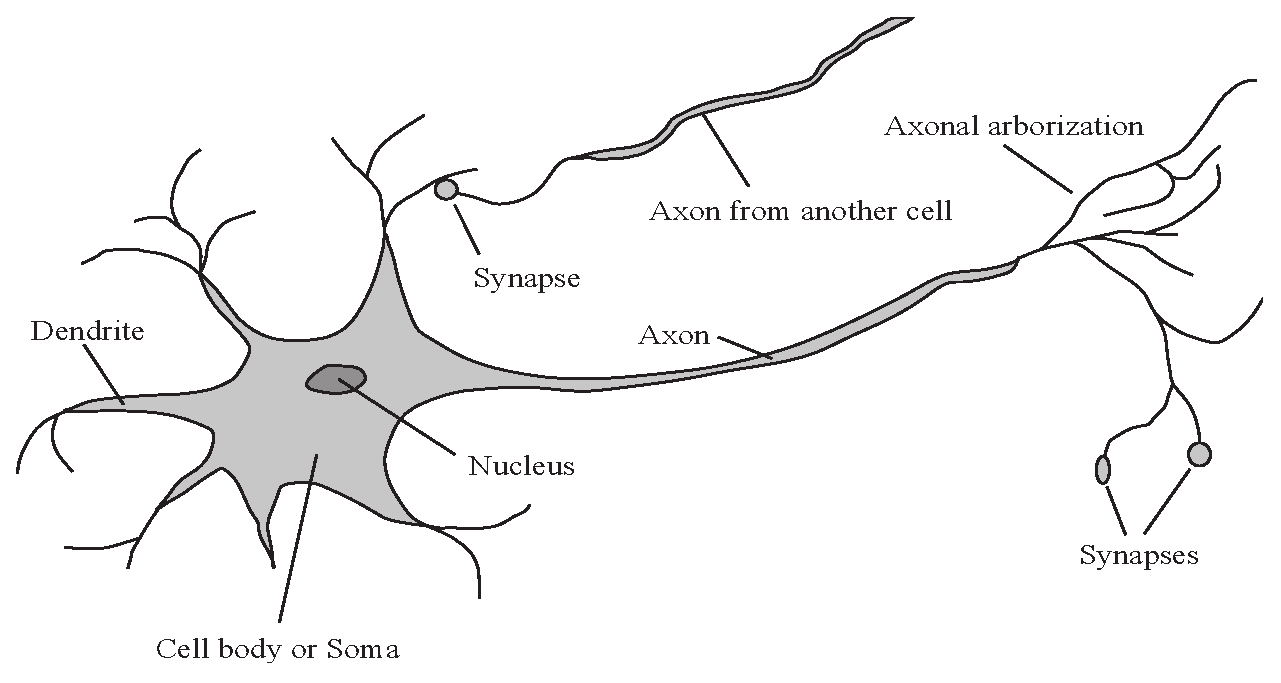
\includegraphics[width=0.95\textwidth]{ModellAvNeuronet.eps}
	\caption{A illustrative model of the neuron. The signal propagation goes from the left to the right in this figure;
			Synaptic integration at the dendrites, action potential through the axon and finally transmission throught the output synapses. 
			The aspects of the cell body is not immediately relevant to signal processing, and is not taken into account in the model used. }
	\label{figFigurAvNeuronet}
\end{figure}

% Gjennomgang, natt til 30juli. Her er eg no.
% TODO TODO TODO TODO TODO TODO TODO TODO TODO TODO TODO TODO TODO TODO TODO TODO TODO TODO TODO TODO TODO TODO TODO TODO TODO TODO TODO TODO TODO TODO TODO TODO TODO 

When the action potential reaches the ``axon terminal'', where the presynaptic membrane of the synapse lies, neurotransmitters are released into the synaptic cleft 
 	(se appendix \ref{appendixSecPresynapticSynapticPartOfTransmission} for a more complete discussion of the action potential and the presynaptic elements of synaptic transmission).
The neurotransmitters diffuse passively out in the synaptic cleft. Some come in contact with the postsynaptic receptors, and activates the receptor.
%The receptors that are relevant to this project is the ligand--gated receptor group.
%Describing the different known kinds of receptors will be outside the scope of this report. We will limit the description to one class of receptors, called ``ligand--gated receptors''.
Directly--gated receptors (also called ``ligand--gated channels'') open a channel when exposed to the right ligand (the right neurotransmittor), 
	causing an increase or decrease in the postsynaptic neurons depolarization\cite{PrinciplesOfNeuralScience4edKAP10}. .
%Ligand--gated receptors are direcly connected to ion channels in the membrane. Opening of these ion specific channels enables some ions to flow throught (depending on what kind of channel the receptor is connected to). 
%Depending on which ions are let through, the neuron is either depolarized (towards zero polarization, less than its resting potential) of hyberpolarized (getting a more negative membrane potential) by the transmission.
Whether the postsynaptic depolarization is increased or decreased by a synaptic transmission defines the synapse as being an excitatory or an inhibitory synapse\cite{PurvesNeuroscienceKAP05}.
%On the postsynapsic membrane in the synapse are different receptors for different neurotransmitters\cite{PrinciplesOfNeuralScience4edKAP10}. 
%The receptors are only activated by some neurotransmitters, and the change in postsynaptic postential varies with what ions the receptor channel is permeable to.

%Since depolarizing the neuron causes firing, the neurons potential is often referred to as the neurons depolarization in the litterature.



\subsection{The Axon and the Action Potential}
\label{ssecTheActionPotential}
In the membrane of the axon we have voltage--gated channels that open if the level of depolarization is more than some value. This value is called the ``firing threshold of the neuron''.
These channels will open and further depolarize the membrane. 
Through passive transmission of the electrical potential, the next voltage gated channels will open as a result of going above the gate threshold. %also go beyond the firing threshold.
This establishes the active aspect of action potential propagation, and results in a self carrying propagating through the axon.
%This establishes the self carrying signal of the axon, and results in an equal depolarization at the different axon terminals\cite{PrinciplesOfNeuralScience4edKAP09}.
An important result of this is that the presynaptic membrane at the synapses recieves an equal depolarization, independent of its location. 
The release of neurotransmitters is a result of this depolarization, and the action potential enshures an equal depolarization of the presynaptic membrane.
This gives that the transmission is dependent only on the synaptic connection, or ``the synaptic weight''\cite{PrinciplesOfNeuralScience4edKAP09}.
%
%This means that sufficient depolarization of the membrane of the axon opens voltage gated ion channels that will further depolarize the membrane. 
%Through passive transmission of the voltage, the signal is distributed to the next voltage gated channels.

%todo skriv mot slutten av paragraf:  The voltage gated channels will only be open for a small period of time.
%There are at multiple kinds of voltage gated channels. The sodium channel opens
For the action potential there are two important voltage--gated channels; The sodium channel and the potassium channel.
The $Na^{1+}$ channel opens faster than the $K^+$, and gives the rising phase of the action potential.
The rising phase of the action potential comes as a consequence of more positively charged $Na^{2+}$ ions outside the neuron causing a strong inward current after opening of the $Na^{2+}$ channels.
Voltage gated $Na^{2+}$ only stay open for about 1 ms before they close.
About the same time as the $Na^{2+}$ channels close, the $K^+$ channels open. 
Because there is a larger concentration of $K^+$ inside the cell, this will cause a more negative potential over the membrane. The neuron is repolarized.
%After some time delay, the $K^+$ channel opens, and at about the same time the $Na^{2+}$--channel close.
%We have more $K^+$ ions inside the cell, so increasing the permeability for $K^+$ will decrease the depolarization over the membrane, or ``repolarize'' the membrane.
%When both channels are closed again we are back at the resting potential of the neuron. %SITER: Bear s:91
After the action potential the membrane potential is ``reset''.
As the electrical potential spead passively to the next site with voltage--gated channels, 
	the refraction period of each voltage gated channel is an impotant mechanism to hinder the action potential from going ``the wrong way''\cite{NeuroscienceExploringTheBrain3edKAP4}\cite{PrinciplesOfNeuralScience4edKAP09}.

To recreate the ionic gradient, the ions are transported back by the sodium--potassiom pump.
As this is a mechanism that use a little time to reset the ionic gradients, we have a little period when the gates have to be closed.
This is the basis for the refraction period of the neuron, a small period of time where action potential cannot be initiated\cite{NeuroscienceExploringTheBrain3edKAP4}.

After firing an action potential, the neuron will also have a short period where it is impossible to exite the cell, called \emph{the absolute refraction period}\cite{PrinciplesOfNeuralScience4edKAP09}.. 
%The refraction period of a neuron usually lasts for a few milliseconds\cite{PrinciplesOfNeuralScience4edKAP09}.
%\cite Bear kap. 4  (s.91, nede) og Kandel kap.9 s 157 (nede)
%TODO TODO TODO TODO TODO TODO TODO TODO TODO TODO TODO TODO TODO TODO TODO TODO TODO TODO TODO TODO TODO TODO TODO TODO TODO TODO TODO TODO TODO TODO TODO TODO TODO TODO TODO TODO TODO TODO TODO TODO TODO TODO TODO TODO 
% Plan: finn referanse på dette, og så sei at eg har matematisk vist det å være sant.
In this project, the author has demonstated matematically that the refraction period is important for limiting the firing frequency of the neuron. 
The analysis is presented in section \ref{ssecValueOfAlpha}.
%In this project the author has formalized that the refraction period is important for limiting the firing frequency of the neuron. The analysis is presented in section \ref{ssecValueOfAlpha}.


%												"close to":  SKRIV OM
The axon is organized as a tree, with a trunk in close proximity to the soma of the neuron, called the axon hillock.
The branches of the ``axonic tree'' are called axon collaterals. 
The elements of the axon that is furthest from the axon hillock is called the axon terminal, and is where the output synapses are located.
%The axon ``ends'' in the axon terminal, where the presynaptic part of the synapse is located.
When the action potential reaches the synapse, a transmission is initialized by the opening of voltage gated $Ca^{2+}$ channels\cite{PrinciplesOfNeuralScience4edKAP10}.
%The signals transmitted in the axon is strictly directional, that is: the signal goes from the axon hillock (close to the neurons soma) to the axon terminals (where the synapses is). 

%ODO Skriv mindre, eller i det minstre mindre kraftige utsagn. Følgande er rett, men kanskje urelevant for denne oppgava?
%You also have modulatory synapses at the axon terminal, that does not contribute to the value of the neuron, only the amount of neurotransmitters released following the next incoming action potential. 
%The modulatory synapse is but an example of the complexity of the simplifications that are neccesary in order to make an artificial neural network.
%In addition we have different time delay for different synapses along the axon, diffuse modulatory systems it the brain with modulatory neurotransmittors, 
%different states as the neurons use the oxigene and nutritients available, etc.






\subsection{The synapse}
\label{ssecTheSynapse}
%\subsubsection{Synaptic Plasticity}
%When the action potential reaches the axon terminal, the size of the signal is thought to be the same as when it first was initialized at the axon hillock.
%This enshures that the distance the action potential has to travel does not affect the transmission at the synapses of the different axon terminals. \cite{NeuroscienceExploringTheBrain3edKAP4}.
Following an action potential, voltage gated $Ca^{2+}$ channels are opened and $Ca^{2+}$ enters the axon terminal.
This causes synaptic vesicles to merge with the presynaptic membrane, causing the content of the synaptic vesicles to be released into the synaptic cleft. %Cite Kandel kap.10
% Forrige to linjer (passer med siste forrige section) ELLER neste linje:
%When an action potential reaches the location of a particular synapse, the membrane potential will cause release of neurotransmittors from the axon terminal (the presynaptic neuron).
%-------------------------------------------------------------------------ordna til hit-------------------------------------------------------------------------------------------------------------------------------------------
The neurotransmitters from the synaptic vesicles diffuse into the synaptic cleft.
If a so--called ligand--gated channel at the postsynaptic membrane is exposed to these neurotransmitters, the channel opens and ions are let thought.
The result is either excitation or inhibition of the postsynaptic node's value, depending on the channel (which ions are let through).
The size of the transmission is based on presynaptic and postsynaptic mechanisms\cite{PurvesNeuroscienceKAP05}.
%The transmission is thought to be a funcion of presynaptic and postsynaptic mechanisms.

\begin{itemize}
	\item Presynaptically, different amount of neurotransmitters can be released from the axon terminal following an action potential.
	\item Postsynaptically, the amount of receptors varies between different synapses. The amount also varies with time. % This is one mechanism of synaptic plasticity.
\end{itemize}

The level of transmission is the background for what is modelled as the synaptic weight in artificial neural networks.
%These two sides of synaptic transmission are important when synaptic plasticity is considered. 
Patterns of long term synaptic plasticity is what is what is percieved as learning in the field of neuroscience \cite{NeuroscienceExploringTheBrain3edKAP25}.
A more comprehensive study of synaptic plasticity is outside the scope of this text, but it should be mentioned that the ion $Ca^{2+}$ is thought important in both presynaptic and postsynaptic plasticity.
The postsynaptic role of $Ca^{2+}$ is important for STDP, which is an important argument for ANN with the capability of calculating the spike time.
%This is important for STDP, which is an important argument for ANN with the capability to calculate the timing of the spike.
For the especially interested, appendix \ref{appendixSynPlast} considers presynaptic and postsynaptic mechanisms behind synaptic transmission and synaptic platicity, with a special focus on the role of $Ca^{2+}$.








% //{ Kommentert ut.  Gave til meg selv når eg skal skrive masteren (liten gave, nesten ingenting)

% //{
%The conclution from the study about 

% % XX MED-noke-om: For now, it is enough to mention that the synaptic weight changes as a multifactorial function based on 
%For now, it is enough to mention that  $Ca^{2+}$ is important both presynaptically and postsynaptically for synaptic plasticity.
% % We will later make use of some of the 
% % XXX Bra, men passer det inn:
%When the action potential reaches the axon terminal, it will open voltage--gated $Ca^{2+}$ channels in the active zone of the terminal, and $Ca^{2+}$ enters the cytosol of the axon terminal of the presynaptic neuron\cite{PrinciplesOfNeuralScience4edKAP10}.












% The signal arriving at the presynaptic membrane is equal for all the synapses, the transmission is not. 
% The transmission varies as a function of many mechanisms. %xxx Dårlig setning!
% For the scope of this text, we will focus on the mechanisms within the neuron. 
% I will refer to the size of this transmission as the weight of the synapse. 
% % Dårlig skrevet, over her.

%In this report the convention used by Rolls and Treves in ``Neural Networks and Brain Functions'' will be used. 
%For any transmission through a synapse between neuron $j$ and neuron $i$, we define the synaptic strength $w_{ij}$. 
%Note that the first subscript refers to the recieving neuron and the last subscript to the presynaptic neuron (the signalling neuron) \cite{TrevesNeuralNetworks}.
%This convention will be used in this text. 







%This does not mean that the transmission for different synapses is the same. At each synapse the connection to the postsynaptic neuron is different. 
%There are many mechanisms behind this, but I will focus on the mechanisms within the neuron:
% //}

%\subsubsection{Presynaptic mechanisms behind synaptic plasticity}
% //{
%$Ca^{2+}$ causes release of neurotransmittors from the presynaptic axon terminal into the synaptic cleft\cite{PrinciplesOfNeuralScience4edKAP10}. 
%Long--term potentiation (LTP) causes a lasting change of the tranmission through the synapse.% On the shorter time scale we have short--time potentiation, called fascilitation and short--time depression (decrease of transmission) called 
%
%The amount of $Ca^{2+}$ inflow, and thus the amount of neurotransmitter release can be modulated by socalled axoaxonic synapses\cite{NeuroscienceExploringTheBrain3edKAP5}, synapses that is connected directly to the presynaptic axon terminal. 
%A transmission here will cause a small increase in the axon terminals amount of $Ca^{2+}$ and ``prime'' the synapse for a transmission. 
%Multiple incoming action potentials in fast succession will have the same effect on the following action potentials and causes what is called \emph{potentiation} (short term increase in synaptic weight)
%\cite{PrinciplesOfNeuralScience4edKAP14}. 
% %Variation of the $Ca^{2+}$ entering the presynaptic axon terminal, for example by ``priming'' the synapse for transmission by axon-synaptic synapses, is one potential mechanism for synaptic plasticity\cite{PrinciplesOfNeuralScience4edKAP14}.

% X XX Ta vekk mykje av "Presynaptic mechanisms behind synaptic plasticity" om eg ikkje bruker desse effektene i implementasjonen!
% //}


%\subsubsection{Postsynaptic mechanisms behind synaptic plasticity}
% //{
%Glutamate is the main excitatory neurotransmittor in the CNS\cite{PrinciplesOfAnatomyAndPhysiology12edKAP12}. %s. 448
%There are two main groups of ligand--gated glutamate receptors, the N-methyl D-aspartate (NMDA) receptors and the non-NMDA receptors. 
%The non-NMDA receptors mainly consists of the $\alpha$-amino-3-hydroxy-5-methyl-4-isoxazolepropionic acid (AMPA) receptor. %XXX SITER!
%
%Most non-NMDA receptors are permeable to ions that changes the postsynaptic potensial without having lasting changes on the synaptic strength.%efficiancy. 
%The NMDA receptor is permeable to $Ca^{2+}$, which is important for lasting changes of the synaptic strength. %uttrykket 'synaptic strength' har ikkje blitt definert enda. Gjør det lenger oppe. XXX DO IT!
%
%An other important difference between the NMDA-R and the AMPA-R is that NMDA receptors have an additional condition for opening of its ion channel. 
%In the NMDA receptor there is a $Mg^{2+}$ ion blocking the channel. 
%When the potential across the membrane is sufficiently depolarized, the $Mg^{2+}$ will float more freely and the block is removed from the NMDA receptor.
%$Ca^{2+}$ diffuses into the cell following an action potential\cite{PrinciplesOfNeuralScience4edKAP12}.
%
%Also on the postsynaptic part of the synapse $ca^{2+}$ has an important role in synaptic plasticity. 
%$Ca^{2+}$ activates production of more non-NMDA receptors for the postsynaptic membrane, resulting in LTP\cite{AMPARtrafficingArtikkel}.%\cite{PrinciplesOfNeuralScience4edKAP12}.
%
% %TODO Det under gjelder jo bare for kvifor vi får positiv vektendring. Skriv dette, eller finn ut forklaringa for negativ vektendring (LTD) som følge at STDP! XXX
%The NMDA-related synaptic plasticity is the background for what is called ``Spike Timing Dependent Plasticity'' (STDP) that will be important later in this text.
% % XXX ikkje "rest of this text." Det er ikkje viktig over alt. Noken plasser.. Kanskje "an important element in this text."?
% %Skriv om hebbian learning, ustabilitet  og at STDP kalles "stable hebbian learning". Sjå rapport i NEVR3004.
% %STDP has also been called ``stable hebbian learning''. This refers to the 

%\subsection{SKRIV OM STDP! Referer til forrige avsnitt}
% %TODO: sjå rapport NEVR3001, NEVR3003.
% %HER ELLER OVER. kjør \label{forklaringBakSTDP}
% //}

%\label{forklaringBakSTDP} %der forklaringa kommer...

%\subsection{Skriv om Dale's  principle}
%At eit neuron kan sleppe bare en neurotransmittor (eller to, fleire). Desse kan gi ulik virkning på ulike receptore, men i utgangspkt. kan man sei at eit neuron enten er excitatory eller inhibitory. 
%Men dette er også feil. Drøft fram og tilbake.. Skriv konklusjonen (til korleis eg gjør det i min implementasjon) i section{implementation}.


% %Because of the boolean nature of the action potential, the transmission of the action potential to the next neuron is desided by the strength of the synaptic connection.

% %The most studied neurotransmittor is glutamate. In most neurons glutamate is an excitatory 

% %Skriv om STDP (glutamate), om bakgrunnen for STDP: NMDA med mg²⁺ blokk, voltage dependent i tillegg til at utsida må være eksponert for glutamat, Ca²⁺ inflow fører til AMPA-syntese => synaptisk plastisitet! 


%\subsection{nettverket}
% - Med booleanske signal: korleis kan signalet inneholde så mykje informasjon?
% 		- skriv om inter-spike period. Og kanskje om ANN-flyttals variablene som output fra neurona..
% //}

\newpage
% Her skal eg skrive om den nye modellen. Kva er \kappa, kva representerer denne, tid går mot uendelig.. osv.

% Disposisjon:
% 
% 1) kva gir depol. for ein neuron. Kva gir input, kva gir lekkasje?
% 2) utledning av depol.-ligning
% 
% 	TODO Lag frampeik om at "dette kan brukes til ANN", eller tilsvarende.
%

\section{Mathematical modelling of the biological neuron} 
\label{secMatematiskModelleringAvBioNeuron}

%Når eg skriver om:
% Fokuser mest på at value, dvs. depol. til neuronet er kva som er viktig i forhold til fyring av AP. Difor bør vi prøve å modellere dette.
% Ikkje tenk på Nernst, her. Det kommer i neste avsnitt.

Mathematical modelling of the neuron helps understand the neuron and the mechansims behind how the neuron works.
The ide behind $\kappa$ANN came as a result of models written to understand the neuron.
A good model could also be used to make a simulator of the modelled effects. 
%A delicate balance is to be mainained between simplifying the system to much, and not simplifying enough.
% TODO Fortsett her. LAg mindre, ikkje større..
% A good model of the neuron will also give us a guide when simulating the system.

In the LIF model of the neuron,  the value of each node is given by the electrochemical potential over the cell membrane. 
%In the neuron, the value of each node is given by the electrochemical potential over the cell membrane. 
The neuron will fire an action potential if the value goes above firing threhold.
This makes the value of the neuron an important aspect of neuronal signal processing.
When a neuron recieves one kind of synaptic transmissions, ligand--gated channels are opened, and the potential of the neuron is changed as a function of the time the channel is open 
	and the electrochemical driving force for the charged molechules.

The electrochemical driving force can be seen as a potential field over the membrane.
This mechansim either comes from the concentration of diffenert kinds of chemical molechules, as a result of electrical potential, or a combination of the two.
%One aspect of this potential is the concentration gradient over the membrane.
Each ion will seek a state of the least order, or the highest order of entrophy. 
The concentration gradient of each ion is therefore an element of the electrochemical driving force for that ion.

The second aspect of the potential field is the electrical potential over the membrane. 
If a particle is charged, we get a situation where nature have a desire to increase the level of entrophy for the charge.
This gives that the charged ions will get a driving force from any compartment or object with the similar charge.

%If we combine these two effects we get a simplified system of the neuron.

% TODO  under. Skriv alt heilt om! What? kanskje eg har gjort det?
In the biological neuron, the value of the node is therefore governed by many factors. 
The individual ion's equilibrium potential can be calculated by the Nernst equation (eq. \ref{eqNernstEquation}).


The electrical potential over the membrane of the biological neuron is given by the distribution of ions or charged particles and molecules over the  membrane.
%The membrane potential of the biological neuron is given by the distribution of electrically charged particles and molecules over the  membrane.
The electrical potential is an important part of the driving force for changing the value of the node.
It also is the prime motivator for the initiation of an action potential, and thus an important aspect to model.
%From this we can later talk about the differential equation of the nodes value.
%The electrical driving force is not the only one, and the value of the node at equilibrium is given by the sum of all these driving forces.





\subsection{The equilibrium potential}
% TODO TODO Skriv også om lekkasje! Fra ANN.tex refererer eg hit når eg snakker om lekkasje. XXX Hugs å skrive om lekkasje her!
% Sjå ANN.tex: Snakker om LIF-neuron. Skriv om LIF-neuron når eg skriver om lekkasjen!
\label{ssecTheEquilibriumPotential}
%TODO Er det her eg skal skrive om LIF-neuron (leaky integration)?
In the biological neuron, the reversal potential for the different ions can be calculated by the Nernst equation. 
%The reversal potential is the electrical potential where the ion flow will be revesed (flow the oposite direction). % if an ion channel is opened.
The reversal potential is the electrical potential where the driving force will be reversed.
As this is a continuous variable, the value for the point of reversal is zero. 
This gives that the reversal potential also could be referred to as the equilibrium potential.
%The reversal potential is the electrical potential where the opening of an ion channel causes the directionality flow to be reversed.


% xxx xxx xxx xxx xxx xxx xxx xxx xxx xxx xxx xxx xxx xxx xxx xxx xxx xxx xxx xxx xxx xxx    Kvalitet er crap, men TA MED FIGUREN I RAPPORTEN!
%\begin{figure}[hbt!p]
%	\centering
%	\includegraphics[width=80mm]{membranePotAtRestFigFromKandel.jpg}
%	\caption{The fluc of the ion $K^+$ across the membrane is determined by both the consentration gradient of $K^+$ and the electrical membrane potential \cite{PrinciplesOfNeuralScience4edKAP07}.
%	\label{figVerdifunksjonen}
%\end{figure}




%When the electrical potential over the membrane is at the level of the reversal potential for some ion, we get no ionic current for this ion following a channel opening.
%This also involves that at the reversal potential, we get no ionic current for this ion following a channel opening.  %TODO les gjennom, og sjekk om det er rett.
When the electrical potential over the membrane is at the level of the reversal potential for some ion, the electrical and chemical driving forces for that ion sums to zero;
The force created by the electrical potential and by the concentration gradient is equal in size but opposite in direction.
% %This is due to a balance between the driving force provided by the concentration gradient of the ion and the electrical driving force.
The equilibrium potential for an ion is given by the \emph{Nernst equation}\cite{NeuroscienceExploringTheBrain3edKAP3}..
%The reversal potential is also called the equilibrium potential\cite{NeuroscienceExploringTheBrain3edKAP3}.

\begin{equation}
	\label{eqNernstEquation}
 	E_{ion} = \frac{C}{z} log\frac{[ion]_o}{[ion]_i}
\end{equation}
Where $E_{ion}$ is the equilibrium potential for the ion, C is a constant (for some constant temperature), z is the charge of the ion and $[ion_i]$,$[ion_o]$ gives the number of ions on the inside and outside of the membrane
\cite{NeuroscienceExploringTheBrain3edKAP3}.

%For a neuron permeable to a single ion, the neuron's equilibrium potential will be the same as this ion's equilibrium potential. %ref kandel kap 7. s129
%For systems where we have permeability to multiple ions, the equations for each ion becomes a sum of electrical driving force and chemical driving force multiplied with membrane conductance for the ion
%For systems where permeability of multiple ions are involved, the equations for each ion becomes a sum of electrical driving force and chemical driving force multiplied with membrane conductance for the ion
%\cite{PrinciplesOfNeuralScience4edKAP07}.
%
%skrive om at dette gir oss at for en komplett simulering av dette, trenger vi en variabel som holder orden på kvart ion.
For a simulation with a high fidelity, the concentration of every ion and electrically charged particle or molecule have to be calculated.
%A good simulation of the system therefore should have one variable for each of the electrically charged particles and molechules.
As there are many ions involved, and some protheins and neurotransmitters are electrically charged, this introduces a large computational load for the simulation.
%There are many important ions and also a couple of protheins and neurotransmittors that are electrically charged, so this will introduce a large computational load in the simulation.
% %Many, if not all of the previous implementations I have seen have a simplified structure for the node's value, by having one activation value; The electrical potential.
To my knowledge, no implementation of SANN with a pragmatic use (i.e. used in technology) uses multiple ions to find the depolarization of the nodes in the simulation.
%These implementations use the electrical potential as the value for each node. This will also be the focus of the remaining part of the modelling section.
All implementations seen by the author use only the electrical potential as the value of each node.
AuroSim will also use only one variable to simulate the depolarization of the node.
The focus of the modelling done in this project thus only use one variable as the value of the node.







% Todo: Skriv om neste linja! 		Ikkje permeabel til noke ion, men litt permeabel for ion.. XXX XXX XXX
As the membrane is selectively permeable to some ions, and makes use of mechansims that pumps ions over the membrane, an electrical potential that differs from the equilibrium potential can be created. %siste 3 ord: endre! xxx
%At rest, the membrane is permeable to some ions, and to prevent the ion reaching (and staying) at the neurons equilibrium potential, there are active pumps maintaining a different potential. 
%
In the postsynaptic membrane of most synapses, there is so--called \emph{ligand--gated ion channels}.
The ligand--gated channels are ionic channels that are activated by exposure the activating neurotransmittor\cite{NeuroscienceExploringTheBrain3edKAP5}.

Activation of a ligand--gated channel will cause it to open and let ions flow through. % the channel.
%The channel will be open for a small time period, causing a flow of the ions that are let throught the channel, giving an altered postsynaptic potential. 
The channel will be open for a small period of time, causing an altered postsynaptic potential.
Excitatory synapses increase the postsynaptic node's value, and is called an Excitatory PostSysnaptic Potential(EPSP). % \cite{PrinciplesOfNeuralScience4edKAP07}.
% 	% 	%
Other ligand--gated channels have channels that decrease the value, due to permeability to other ions.
%Other ligand--gated channels have other channels that will decrease the value of the neuron.
% %Inhibitory synapses have other channels that causes an inhibition of the postsynaptic neuron. 
As this inhibits the neuron in respect to firing an action potential, these synapses are called inhibitory synapses\cite{PrinciplesOfNeuralScience4edKAP07}.
%The postsynaptic effect of a transmission is called an Inhibitory PostSynaptic Potential(IPSP). 		%HER er eg. XXX XXX
%Because this inhibits the neuron in respect to firing an action potential, this is called inhibitory synapses, and the postsynaptic effect of a transmission is called Inhibitory PostSynaptic Potential (I--PSP).
%This involves decreasing the postsynaptic neurons value. This is called an Inhibitory PostSynaptic Potential (I-PSP).
%XXX ref kap 7. kandel.

%Because of time limitations, modelling of the time delay and size of each transmission has not been evaluated in this project.
%Another aspect that will be for further research, is modelling and implementation of synaptic plasticity. 
%This is one important reason behind using artificial neural networks in technology, and the reason behind developing the spiking variant of ANN.
%Synaptic plasticity will hopefully be modelled and implemented in a later project.
% %This project is about the comparison between 

%Opening of a membrane channel will change the permeability of the membrane to some ions (depending on the channel), and the ion pumps will not be able to maintain the potential different from the equilibrium potential. 
%This causes the potential of the neuron to change accordingly, and is the basis of excitatory and inhibitory postsynaptic potentials (E-PSP/I-PSP)\cite{PrinciplesOfNeuralScience4edKAP07}.
%X XX ref kap 7. kandel. s. 131



Some of the aspects introduces here was included to demonstrate the complexity of the simulated system, even at the level of the indivitual node.
%Some of the aspects in the theory of the electrical potential for the neuron was introduced to show that the simulated system is a complex one, even at the level of the individual node. 
%For each node we have a complex system with a continuously changing driving force and membrane conductance for each ion. 
In ANN, we can simplify the neuron and only use one variable to describe the state. 
This is done for the sake of efficiancy.
%For artificial neurons used in an ANN most of these aspects can be simplified without affecting the result much. 
Because the primary focus for this implementation is the use of the neural simulator in technology, the efficiancy of the implementation is crucial. 
%We therefore have a single variable giving the membrane potential as the activity variable in this implementation. 
We will therefore use only one variable to give the membrane potential of teh node.
The extra computational load introduced by multible activity variables makes the simulation to computationally demanding for ANNs with a pragmatic focus. 

%It is also important to know about the complex structure of neural signal processing





Until now, this chapter has introduced different aspects important for modelling the behaivor of the neuron.
The next section, and the remainder of this chapter will be used to describe the modelling done in this project.
The equations found in this section will be of importance later, when we discuss the new model for ANN.


% //{ Kommentert ut. Har ikkje tid å fikse..
%$V_{r}$ will be used as the resting membranes potential. For biological neurons this can be calculated by the Goldman equation\cite{PrinciplesOfNeuralScience4edKAP07}. 
%For our use if will be enough to know the extistance of the equilibrium potential for a membrane at rest,
%in addition to define a resting membrane potential for the implementation of the artificial neuron.
%
% %For multi--ion systems modelling the system becomes more complicated, but for our use it is enough to know that there is a resting membrane potential that is a function of


% TODO Minimaliser reperering av det er nettop har sagt.. XXX
%
% %It is important however to know that there is such an equilibrium potential, given by the sum off all the contributions (from the individual ions).
%
%Because of the active pumps, different states with different permeability do the different ions will give different membrane potential because of different factors for each part of the ion differential equation. 
%The membrane at rest, that is with no open ion channels, gives the resting membrane potential, $V_r$. 
%
%In the case of synaptic input to a neuron, the postsynaptic membrane will open ligand gated channels (se section \ref{ssecTheNeuron}). 
%Both for excitatory and inhibitory input this will push the neurons value and could be seen as an external force in the system.
% %For our use, we set this external force to be a constant.
%Whether this external driving force can be percieved as a constant or is a more complicated dynamical system is as everything else in the nature; complicated. %Skriv slutten analeis.
%The neuron has NMDA channels that are more permeable to both the normal ions in addition to $Ca^{2+}$. Since the NMDA-R is voltage dependent, this causes the glutamatic transmission to be a function of the postsynaptic potential.
%
% %For E input. Kva skjer. Sjå på som eksternt pådrag. 
%As this is a mechanism that is little described in articles in neuroscience and to my knowledge not used in ANNs, I will not use voltage dependent excitatory ion channels in my two implementations of ANN. 
% %Skriv at dette uansett ikkje har noko innverkning på resultatet? Eller blir dette også dumt i forhold til relevansen til denne linja i teksten?
%For my implementations the external driving force on the membrane potential will in other words be a constant.

% %Skriv om lekkasje. Forbered på neste seksjon.
% %When the potential over the membrane does not equal this equilibrium potential, the system will be driven toward this equilibrium. %(without any external input).

% %In the case of neural networks, this is called a 'leaky integrate-and-fire' (LIF) model.
% //}







\subsection{The differential equation for neurons depolarization} 
The equation for the potential can be stated as a first order differential equation:
\begin{equation}
	\dot{v}(t) = \dot{v}_{in}(t) - \dot{v}_{out}(t) %, \qquad i = \text{ neural input } %% XXX Endra \dot{v}_{in}(I) til  \dot{v}_{in}(t). XXX
	% skriv også at det er \dot{v}_{out]}(t, v(t)) ---avhengig av v(t) også!
\end{equation}
Where $\dot{v}_{in}(t)$ gives the effect of synaptic input to the neuron and $\dot{v}_{out}(t)$ represents the ``leakage'' of the neurons value.



% TODO Ikkje del opp i underavsnitt: Skriv heller "Element for diffligninga", eller noke, og få med begge her.
% Men det eg heller kan ha med som underavsnitt er "forkrav for ligningene" eller "utgangspkt" eller "antagelser for ligningene"...
\subsubsection{The input}
The input, represented by $\dot{v}_{in}(i)$ in the above equation, is a function of the neurons excitatory and inbibitory input. 
The neurons input waries in time, but for now we look at the variable $I$ as a constant.
%One method for a varying degree of input will be introduced in section \ref{ssecVariableInputBetweenSpikes}.
Later, in section \ref{ssecVariableInputBetweenSpikes}, a method will be presented for changing the level of input.  % expanded to account for a varying degree of input. % (section \ref{ssecVariableInputBetweenSpikes}).
%Later, in section \ref{ssecVariableInputBetweenSpikes}, the method will be expanded to account for a varying degree of input. % (section \ref{ssecVariableInputBetweenSpikes}).

\begin{equation}
	\dot{v}_{in}(t) = I
\end{equation}
%$I$ is the effect of the input to the neuron (sum of excitatory and inhibitory input).
$I$ represents the effect of the synaptic input to the neuron; 
	The sum of the effect of all excitatory and inhibitory input to the neuron.

%skriv også at v_in(i) er i virkeligheita eit dynamisk forløp, men for ANN kan vi forenkle, og sjå på denne som konstant.


\subsubsection{The ``leakage''}
%TODO Finn referanse for neste påstand!
The neuron is often modelled as a leaky integrator. 
The ``leakage'' varies with the value of the neuron. % polarization over the membrane. 

For biological neurons, the leakage is given as a function of the difference between the membrane potential and the resting membrane potential $V_r$. 
If we define the resting membrane potential for our artificial neuron to be zero, the leakage will vary propotionally to its potential $v(t)$.

\begin{equation}
	\dot{v}_{out}(t) = \alpha v(t)
\end{equation}

In a biological neuron, the propotionallity constant $\alpha$ is given by 
	the permeability to different ions at rest, 
	the active pums, 
	the difference in the ionic environment between the extracellular and the intracellular compartment, 
	etc.
%In a biological neuron, the propotionallity constant $\alpha$ is given by the distribution of different ion channels active at rest, the extracellular ionic environment compared to the intracellular level of the different ions, etc.
For the simplified neuron used in this model, $\alpha$ will be a constant. % will be kept constant. 
%For our basic ANN this will be cept constant. 
% % IDE: For more advanced versions of this simulator, $\alpha$ could vary as a function of the intracellular ion--levels. 
%In addition we have that the extracellular ionic environment is to large extent maintained by glial cells.
% %In the CNS you have so--called astricytic domains governed by astrocytes (a certain kind of glial cell). In this domain the 
% BRIFEKUNNSKAP:XXX :  In the CNS you also have socalled astrocytic domains, where the support--cells for the neurons have domains. Inside this domain one astrocyte is 


\subsection{The depolarization equation}%equation for the neurons value}
%\label{ssecDepolEq}
%This gives us the differential equation 
The differential equation is given by:
\begin{equation}
	\dot{v}(t) = \dot{v}_{in}(I) - \dot{v}_{out}(t) = \, I - \alpha v(t)
\end{equation}

Laplace transformation gives
% XXX Legg utledning av uttrykk i appendix! 		Her skal bare stå: V(s) = ...
\begin{equation}
	\begin{split}
		sV(s)-v_0 		&= \frac{I}{s} - \alpha V(s) 			\qquad, \; \qquad v_0 = v(t_0) 				\\
		(s+\alpha)V(s) 	&= \frac{I}{s} + v_0 														\\
		V(s) 			&= \frac{1}{s+\alpha}\left( \frac{I}{s} + v_0 \right)
	\end{split}
\end{equation}

And 
% XXX Legg utledning av uttrykk i appendix! 		Her skal bare stå: V(t) = ...  XXX type: bare siste linja i den kompilerte DVI'en
\begin{equation}
	\begin{split}
		v(t)  	&= 		\mathscr{L}^{-1}\bigg\{ V(s) \bigg\}  									\\
		 		&=		\frac{I}{\alpha} - \frac{I}{\alpha} e^{-\alpha t} + v_0 e^{-\alpha t} 	\\
				&= 		\kappa \left( 1 - e^{-\alpha t} \right) + v_0 e^{-\alpha t} 	\quad,\; \kappa = \frac{I}{\alpha} 
		\label{eqVerdiligninga}
	\end{split}
\end{equation}

% DETTE ER ALLEREDE SAGT: at den blir resatt til null..
% %The diversity of neurons makes it unrealistic to generalize over all neurons, and say to what the value is reset to.
%For our artificial neuron we can define 
% %Generalization for all neurons is unrealistic due to the divesity of neurons, but for our synthetic neurons we can define
%that the neuron is reset to what corresponds to the equilibrium potential at rest, $V_r = 0$ after firing an AP.
% %In the simulated neurons this means that after firing, the neuron is reset to $v_0=0$ after firing. 
%This simplifies further calculations.

We get that the final value of $v(t)$ is given by $\kappa$: 
\begin{equation}
	\lim_{t\to\infty} v(t) = \kappa
	\label{eqKappaSomFinalValueAvV}
\end{equation}
%An other way to look at it, is to say that $\kappa$ is the final value of $v(t)$.

The above equations are only valid for a constant $\kappa$. 
As the value is reset at the time of firing, we get that eq. \eqref{eqVerdiligninga} can be used within one inter--spike period(the period between consecutive action potentials).
The time $t$ then gives the time relative to the previous firing.

%The action potential is a discontinuity in the othervise continuous system. The continuous equation is only valid between action potentials (within one period).
% %If we reset every aspect of the equation to be reset after firing, the equation can be used for the discontinuous system. 
%To use \eqref{eqVerdiligninga} for the whole time range, we define $t = t_{abs}-t_f$, where $t_{abs}$ is the absolute time and $t_f$ is the time of the last action potential. 
%In this way $t$ represents the time since the start of the current period.



%Equation \eqref{eqVerdiligninga} describes a continuous nonlinear system. 
%In the neuron we have that if the neurons value goes above some threshold the neuron will fire an action potential, and the value is reset. This introduces yet another nonlinearity: 
%The action potential.

\subsection{The Action Potential}
The action potential, a ``spike'', and the period between action potentials, the interspike period, is the basis of the computational capabilities of the neuron.
When the value of the neuron excedes the firing threshold an action potential is initialized, causing transmission at all the neuron's output synapses and resetting the neurons value.
%This causes transmission at all the output synapses of the neuron, and resetting the value of the neuron to $V_r$. % = 0. Skrive at det er lik null. Gjør likningene under rett..

We get that the neuron fires at time $t^*$:
\begin{equation}
	\begin{split}
			v(t^*) 					 							&= \tau \qquad 										\\	%,\qquad\qquad\tau = \text{firing threshold} 	\\
			\kappa (1-e^{-\alpha t^*}) + v_0 e^{-\alpha t^*})	&= \tau 											\\
	%		(v_0-\kappa)e^{-\alpha t^*}							&= \tau-\kappa 										\\
			e^{-\alpha t^*} 			 						&= \frac{\kappa - \tau}{\kappa - v_0} 					\\
			t^*													&= -\alpha^{-1} \, \ln \left( \frac{\kappa - \tau}{\kappa - v_0} \right) 					
	\end{split}
	\label{eqTidTilFyringVedEndraKappa}
\end{equation}

Where $\tau$ is the firing threshold of the neuron. 
% % ( Skriv at i tillegg får vi den såkalla "refraction time" errer eit AP. Dette må legges til for å få heile perioden.
% % % %
%If we define $p_d(\kappa)$ as the depolarizing phase of the inter--spike interval, the depolarization phase of the period is given by
The depolarization phase of the period is given by
\begin{equation}
	p_d(\kappa) = -\alpha^{-1} \, \ln(\frac{\kappa - \tau}{\kappa})
	\label{eqPeriodeligningForKonstIntraPeriodKAPPA}
\end{equation}
We have used that $\kappa$ is constant in the inter--spike interval, which gives that $v_0 = 0$.

Equation \eqref{eqTidTilFyringVedEndraKappa} can also be used to calculate the time until firing for a given $\kappa$ and start value $v_0$
\begin{equation}
%	\begin{split}
	p_{r}(\kappa, v_0) 	\;= t^* + t_r 
						\quad= -\alpha^{-1} \, \ln \left( \frac{\kappa - \tau}{\kappa - v_0} \right) + t_r
%	\end{split}
	\label{eqRemainderOfPeriod}
\end{equation}
Here $p_r(\kappa, v_0)$ represents the remainder of the current inter--spike period and $t_r$ the absolute refraction period. % TODO XXX Skrive om dette? :  To see the refration time as a constant is a simplification.
As we calculated a new firing time every time eq. \eqref{eqVerdiligninga} is used, the refraction period has to be added each time the firing time is calculated.
The refraction period is more complex than the constant used in this model. For an example of more elaborate modelling of the refraction period, it is referred to \cite{Kunkle02pulsedneural}.
%The refraction period is more complex than so, but for our simple model we use this model of the refraction period.

It is important to remember that equation \eqref{eqPeriodeligningForKonstIntraPeriodKAPPA} and \eqref{eqRemainderOfPeriod} is based on a constant $\kappa$ during the whole period. 
% Det er meir komplisert enn det som står på neste linje. (gjør det litt større).
If $\kappa$ varies during the interspike period, the firing time will also change. 




\subsection{Variable input between spikes}
% TODO Skriv heilt om!
\label{ssecVariableInputBetweenSpikes}
%Equation \eqref{eqPeriodeligningForKonstIntraPeriodKAPPA} is based on a constant $\kappa$ during the inter--spike period.

%If $\kappa$ needs to be constant during the whole period, we get a large time lag for the system, so we need to devise a scheme for avoiding this.

If $\kappa$ varies during the inter--spike period, eq. \eqref{eqVerdiligninga} and \eqref{eqTidTilFyringVedEndraKappa} can not be used directly.
%If we allow the activation level of the node to change during the inter--spike period of the neuron, we cannot use \eqref{eqVerdiligninga} and \eqref{eqTidTilFyringVedEndraKappa} directly.
To avoid this limitation, the concept of a ``time window'' is introduced. 
%A time window is defined as a period of time where $\kappa$ is constant, within one interspike period.
\begin{mydef}
A time window is a time interval where $\kappa$ is constant, within one interspike period.
\end{mydef}
%
We get that a time window is defined as the smallest of [a time interval where $\kappa$ is constant] or [the remainder of the interspike period].
%To solve this problem, the concept of a ``time window'' is introduced. A time window is defined as the smallest of [a time interval where the activation level of the node is constant] or [the remainder of the interspike period].
%Within each time window both \eqref{eqVerdiligninga} and \eqref{eqRemainderOfPeriod} is therefore valid. % .. kan bli brukt.
As $\kappa$ is constant within a time window, equation \eqref{eqVerdiligninga} and \eqref{eqRemainderOfPeriod} is valid within a time window.
%Both equation \eqref{eqVerdiligninga} and \eqref{eqRemainderOfPeriod} is therefore valid within a time window.

\begin{figure}[hbt!p]
	\centering
	\includegraphics[width=0.95\textwidth]{demonstrasjonAvUlikeKappaforVerdifunksjonen}
	\caption{$v(t)$ for changing $\kappa$. $\kappa_0=0.7$. At time $t_p=100$ $\kappa$ changes to $\kappa_1=0.5$. 
			At time $t_p=150$ $\kappa$ is set to $\kappa_2=1$.}
	\label{figVerdifunksjonen}
\end{figure}


When $\kappa$ is changed, a new time window is initialized.
This is done by saving the time of initiation and calculating the initial value $v_0$ for the new time window.
The inital value can be found by calculating the value of the neuron when $\kappa$ is changed.
This can be done by eq. \eqref{eqVerdiligninga}.

As eq.  \eqref{eqTidTilFyringVedEndraKappa} is valid within a time window, the firing time of the node can be calculated. 
The word ``estimation'' is used because we can not know whether $\kappa$ will change before this time.
If $\kappa$ is changed before the estimated firing time, the firing time will be affected. 


% Gammel versjon:
%When $\kappa$ is changed, the initial value of the next time window, $v_0$, can be calculated from \eqref{eqVerdiligninga}. 
%We can now use \eqref{eqTidTilFyringVedEndraKappa} to find the new estimate for the firing time of the node.
%I use the word estimate because we can not know when $\kappa$ will change.
%If $\kappa$ is changed before the estimated firing time, the firing time will be affected. 

%Equation \eqref{eqTidTilFyringVedEndraKappa} gives us the time of firing for a situation where the initial value of the node can be different from zero.
%Also this equation is based on a constant $\kappa$.

% //{ Anna fra gammelt av..
%The equations can also be used as the non--linear activation function for a fANN. This activation function is based on a mechanistic model of the biological neuron.
%The activity can be read out of eq. \eqref{eqPeriodeligningForKonstIntraPeriodKAPPA} as the frequency $f(t) = \frac{1}{p(\kappa)}$
%
%If we let the activity level vary between spikes, the model will give as accurate timing as ``Spiking Artificial Neural Network''(SANN). We will discuss different aspects of artificial neural networks later. %XXX Ref?
%The model is based on fundamentally different equations than the model for SANN. 
%If this new model is as effective or more effective than SANN this project will be a contribution because we calculated the firing time in a new way.
%%Ta vekk siste, forrige linje?

%Another aspect with this new model is that it lies between the two prior models of ANN, and can easily communicate with both.

% If we allow the input and activity of each neuron to vary between spikes, the model approaches the model for the biological neuron.
% When $\kappa$ is updated, a new time window starts. 
% $v_0$ from \eqref{eqVerdiligninga} now represents the value at the start of the time window ( $v_0 = v(t=0)$ ). 
% This value is equal to the value $v(t)$ at the time of change of $\kappa$ from the previous time window(se fig. \ref{figVerdifunksjonen}).
% This is equal to the value of the neuron at the time of variation of $\kappa$ (the value at the end of the previous time window).
% //}

In fig. \ref{figVerdifunksjonen}, $v(t)$ is simulated for three different time windows. 
At time $t_p=100$, $\kappa$ changes from $\kappa_0=0.7$ to $\kappa_1=0.5$. 
At time $t_p=150$, $\kappa$ is set to $\kappa_2=1$. 
Figure \ref{figVerdifunksjonen} implies that the value function is a continuous function that converges toward the updated $\kappa$. %, also when $\kappa$ varies.


With the concept of time windows, eq. \eqref{eqTidTilFyringVedEndraKappa} can be used to calculate the remaining part of the neurons period after $\kappa$ changes value. 
%With this new use of eq. \eqref{eqVerdiligninga}, we can calculate the remaining part of the neurons period after $\kappa$ changes value. 
%The remaining time of the period is given by equation \eqref{eqTidTilFyringVedEndraKappa}, given constant $\kappa$. 
%TODO Finn rett ordbruk, neste linje:
If the value of the neuron is updated every each time $\kappa$ varies, it is possible to estimate the firing time of the neuron whenever needed. %at any time in the course of the simulation.
%If this is updated each time $\kappa$ varies, we always have an estimate of the remaining time based on the present $\kappa$.
%If this is updated each time $\kappa$ varies, we will always have an estimate of the remaining time based on the present $\kappa$.

%Skrive at dette plottet IKKJE er fra kjøring av programmet?




%TODO Finn eit bedre navn på denne subsubsection.
%\subsection{The constants in the depolarization equation}
\subsection{Some final comments}
\label{ssecValueOfAlpha}

The inter--spike interval for a neuron consists of two phases. 
The absolute refraction period and the depolarizing phase (se sec. \ref{ssecTheActionPotential}).
% % % 
Equation \eqref{eqPeriodeligningForKonstIntraPeriodKAPPA} models the interval of the depolarizing phase of the neuron. % , $p_d(\kappa)$.
The equation for the whole inter--spike interval is given by
\begin{equation}
	p_{isi}(\kappa) = p_d(\kappa) + t_r
	\label{eqHeilePerioden}
\end{equation}

Where $t_r$ is the refraction period of the neuron. % , and $p_d(\kappa)$ is given in \eqref{eqPeriodeligningForKonstIntraPeriodKAPPA}.
If we consider the firing frequency of the neuron, $f(\kappa) = p_{isi}^{-1}(\kappa)$ we can see that the asymptote is given by
\begin{equation}
	\begin{split}
		\lim_{\kappa->\infty}{ f(\kappa)} &= \lim_{\kappa->\inf}\left( \frac{-\alpha}{\ln \left( \frac{\kappa - \tau}{\kappa} \right) - \alpha t_r} \right)   \qquad = \frac{1}{t_r} \\ 
		%\lim_{\kappa->\infty}{ f(\kappa)} &= \frac{1}{t_r}
	\end{split}
	\label{eqFrekvensLlim} 
\end{equation}

From this analysis it can be concluded that the refraction period of the neuron will limit the output frequency of the neuron.
This can be seen in fig. \ref{figFrekvensMedOgUtenRefractionPeriod}.

%We can see from this analysis that the refraction period of the neuron is fundamental for restricting the neurons output frequency (se fig. \ref{figFrekvensMedOgUtenRefractionPeriod}).
For biological neurons, the maximum firing frequency is about 1000 Hz \cite{NeuroscienceExploringTheBrain3edKAP4}. %s 79
\begin{equation}
	\lim_{\kappa->\infty}{ f(\kappa}) \approx 1000 \, \text{Hz}
\end{equation}
%If we define the maximum firing frequency to be 1000, equation \ref{eqFrekvensLlim} gives us the absolute refraction period as
If we define the maximum firing frequency for the artificial neuron to be 1000 Hz, from equation \ref{eqFrekvensLlim} we get the corresponding refraction period $t_r$:
\begin{equation}
	t_r = \frac{1}{1000 \text{Hz}} = 1 \, \text{m}s %= 0.001 s = 
\end{equation}

%TODO Skriv at dette er en kjendt størrelse i neuroscience (finn, referer), og er en indikasjon på rettheten til lingningene (?)
% 		Kanskje også skrive litt om at dette er "absolute refraction period". Det er også en mild refraction period etter dette (finn,referer). Dette kan implementeres ved 2ms refraction period for auronet. 
% 		TODO TODO Sjekk andre linja her, og gjør en bestemmelse i forhold til mine ANN. (1 eller 2 ms refraction period?).
If we define the time step of the simulation to be 1 m$s$, the refraction period will be one time step in the simulation.
%With a time step of 1 m$s$, the absolute refraction period (the time interval where it is impossible to exite the neuron) can be set to one time step. 
With a time step of 1 m$s$, the simulation of the refraction period can be done by blocking the input for the durion of one time iteration.
%For SANN nodes, this means that the node will not change its value for the duration of the next time step. 
%For $\kappa$ANN this can be implemented more effective by incrementing the estimated firing time by one time iteration. 


% Plott av frekvens med, og uten refraction period:
\begin{figure}[bhtp]
	\begin{center}
		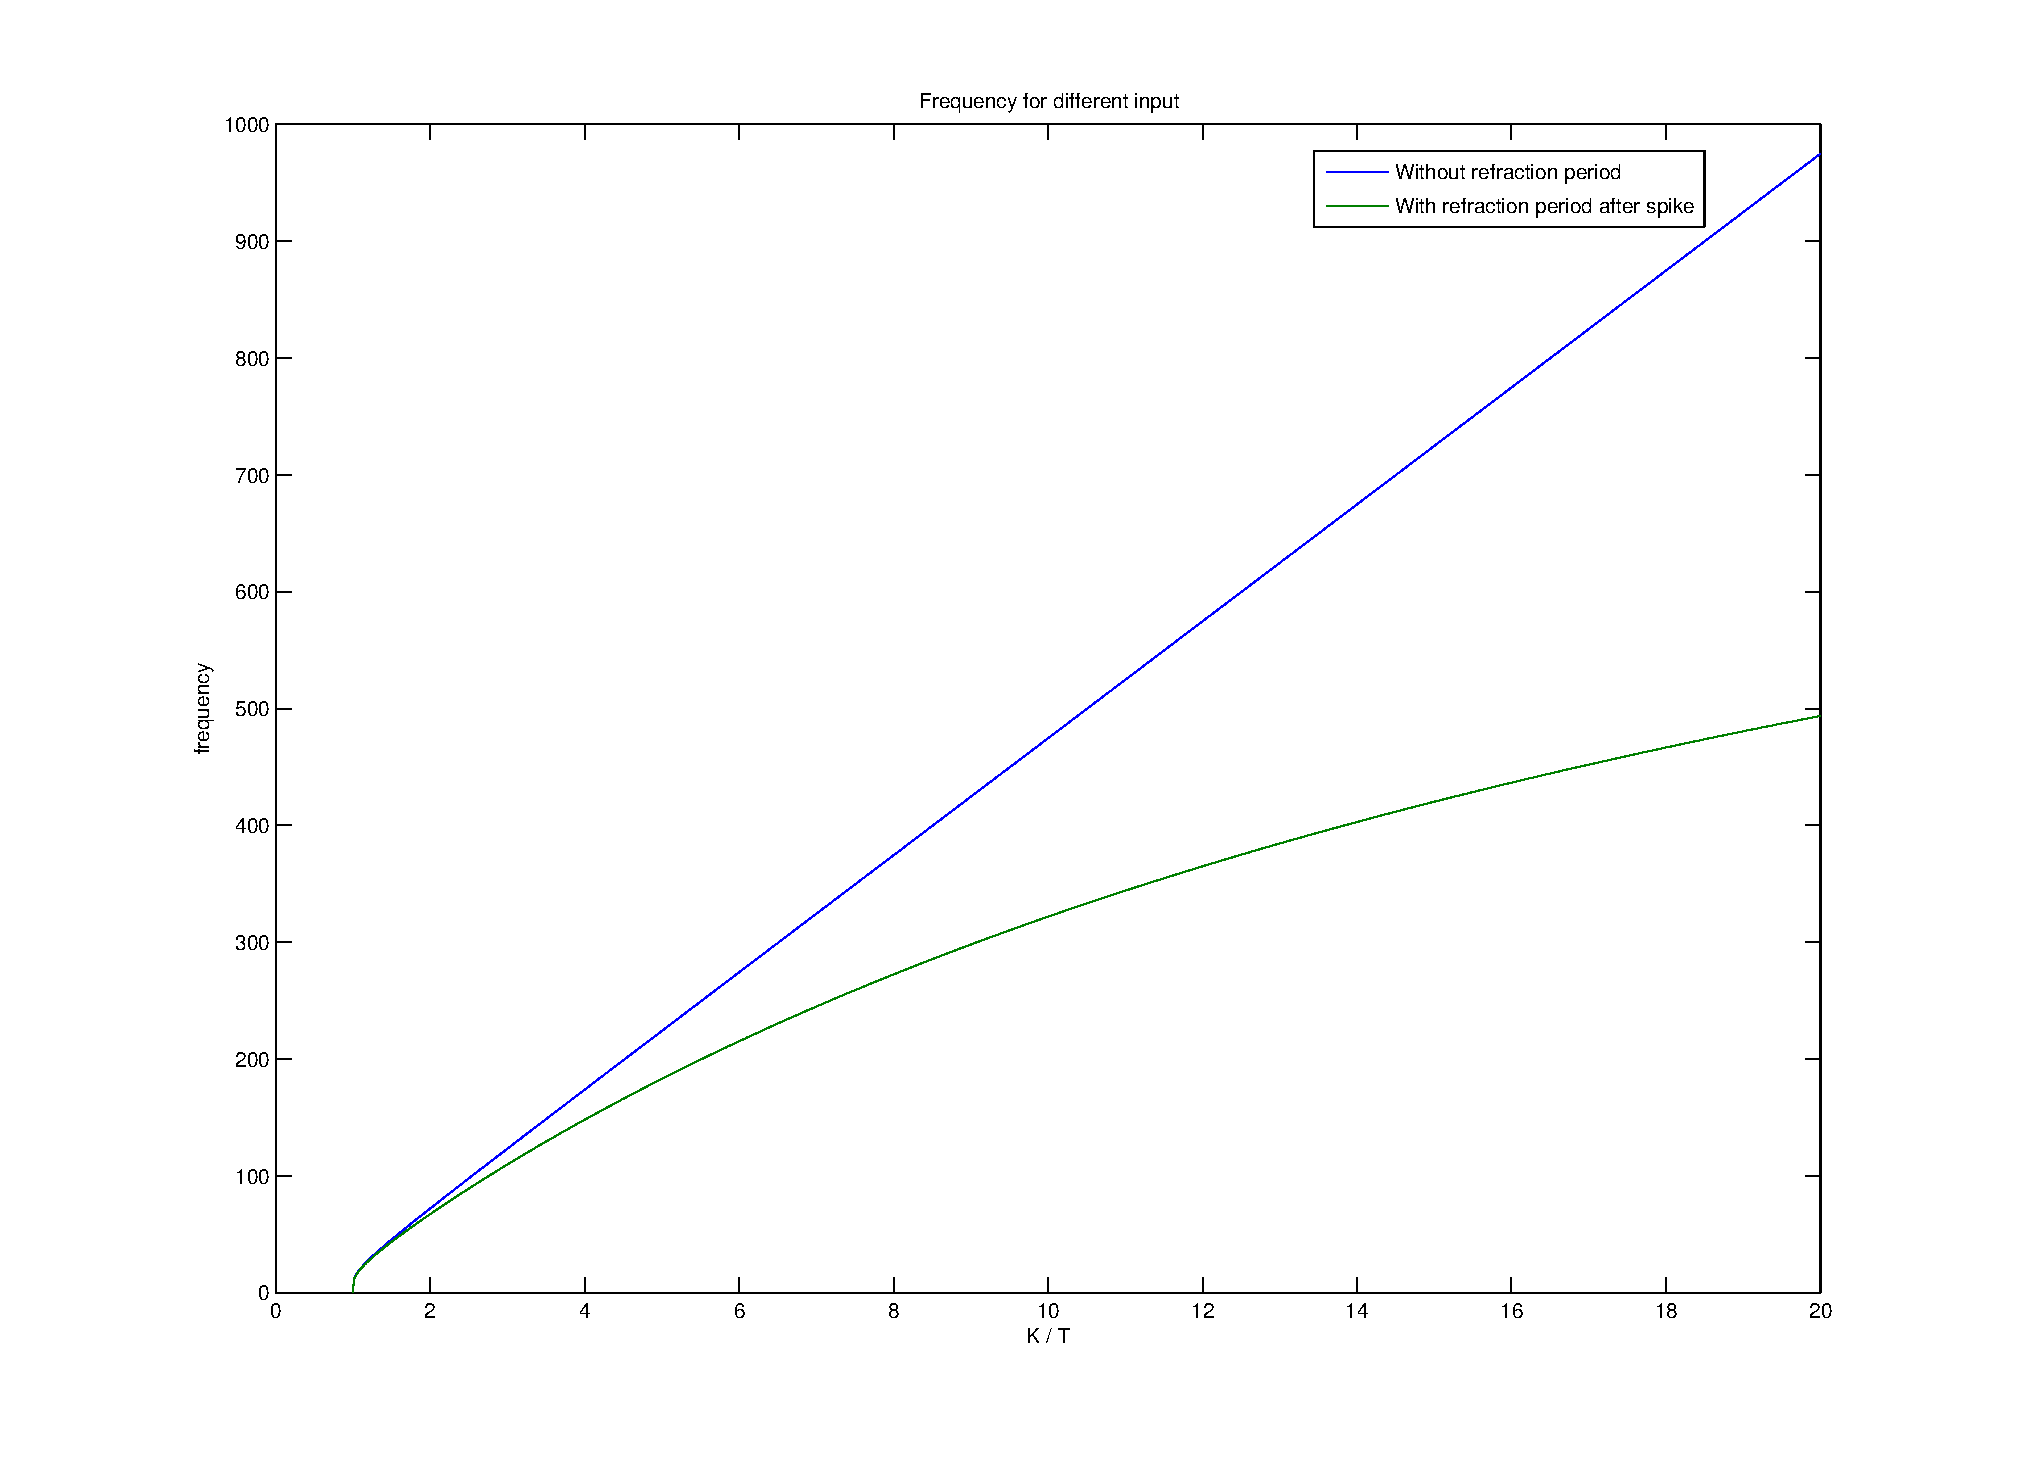
\includegraphics[width=0.95\textwidth]{frekvensPlotRefractionPeriod}
	\end{center}
	\caption{Frequency for a neuron, with and without refraction period for the neuron.}
	\label{figFrekvensMedOgUtenRefractionPeriod}
\end{figure}



%TODO Skriv meir om kva de ulike variablane betyr. Kva er \kappa! kva er \tau,\alpha. Skriv om v_0 for tidsvinduet (referer mykje til rett section)



%TODO Skriv om høgare syn på systemet. Kva betyr Kappa (=ett slags mål på input/lekkasje), output gjennom utsynapser er en funksjon som avhenger av [syn.weight]/[isi_intervall].
% 		- får dermed en { alpha*w_{ij} / ln(1-(T/K)) } relasjon mellom neuronets aktivering (K) og neste neurons input. Bør kanskje lese deg opp på "log-summering som multiplikasjon"-artikkelen, og referere!






%********************************************************************************************************************
%********************************************************************************************************************
%*********************     Trur firing cycle skal vekk!  Evt. finn ut korleis det basser inn.  **********************
%********************************************************************************************************************
%********************************************************************************************************************

%mulighet: Kan skrive om det som en måte å visualisere en ide. Sjå for seg en firing cycle, kvar gang $\kappa$ blir oppdatert, regnes \theta ut. Dette gir oss muligheten for å holder oversikt over fase for signalet.
% skriv om firing cycle som eit konsept, tankebane.






%For this we need to introduce a new concept called the firing cycle.

%\subsubsection{The firing cycle}
%(Skriv om firing cycle, men at det er bedre å regne det ut fra verdien fra eq. \eqref{eqVerdiligninga})

%Because of the cyclic nature of the neurons depolarization, it is possible to visualize the neurons interspike period as a firing cycle.
%If we view this as a cycle, the angle $\theta$ can represent the normalized depolarization of the neuron.

%By defining $\omega(\kappa) = \dot{\theta}(\kappa)$ as a function of $\kappa$ over an infinitesimal period of time, the presumption of constant input over the period becomes more realistic. 
%$\kappa$ will then be used to find the derivative of the depolarization of the neuron. For discrete--time systems this infinitesimal period means the least possible time step, one time iteration.

%If we define 
%\begin{equation}
%	\omega(\kappa) = \frac{1}{p(\kappa)}
%\end{equation}

%Since $\omega = \dot{\theta}$, for constant $\kappa$ over some time interval we have that: 
%\begin{equation}
%	\begin{split}
%		\theta^* = \int_0^{t^*} \! \omega(\kappa) \, \mathrm{d}t 		&= 		\int_0^{t^*} \! \frac{1}{ p(\kappa) } \, \mathrm{d}t 	\\
%					\left[\omega(\kappa)\right]_0^{t^*} 				&= 		\left[ \frac{1}{p(\kappa)}\right]_0^{t^*} 				\\
%																	&= 		\frac{t^*}{p(\kappa)}
%	\end{split}
%\end{equation}
%
%We see from this equation that as $t^* = [0,p(\kappa)]$, we have that $\theta=[0,1]$.
%
%Thus $\theta$ represents the normalized depolarization of the neuron. If we for some reason needs to find the depolarization of the neuron this can be calculated by
%\begin{equation}
%	v(t^*) = p(\kappa) \theta^*
%\end{equation}



%If we further introduce the possibility to change $\omega$ an any time during the period, we can sum the contribution of each period with constant $\kappa$:
%%XXX kan vi anta at \theta_0 + \int_0^t \theta dt = \int_{t_0}^t \theta dt ? : JA siden kappa er konstant så varierer ikkje det inne i integralet med integranten (dt)
% 																																									eller ?
%\begin{equation}
%	\begin{split}
%		\theta_{new} = \theta_{old} + \int_{t_0}^{t^*} \! \omega \, \mathrm{d}t 	\qquad \text{stemmer dette?} %	&= 		\int_0^{t^*} \! \frac{1}{ p(\kappa) } \, \mathrm{d}t 	
%	\end{split}
%\end{equation}

%For a discrete--time system the smallest timestep is defined as one time iteration. For such systems we get:
%\begin{equation}
%	\begin{split}
%		\theta^* = \sum_0^{t_n^*} \! \omega  		&= 		\sum_0^{t_n^*} \! \frac{1}{ p(\kappa) } 	\\
%					\left[\omega\right]_0^{t_n^*} 	&= 		\left[ \frac{1}{p(\kappa)}\right]_0^{t_n^*}	\\
%													&= 		\frac{t_n^*}{p(\kappa)}
%	\end{split}
%\end{equation}

%NESTE: Skriv korleis vi kan la input variere når vi gjekk ut fra at input var konstant. 	-- 'Firin cycle'











%XXX XXX XXX kva er forskjellen mellom denne modellen og SANN? Denne modellen holder input fra kvart inputneuron konstant mellom dets spiker(?) mens SANN holder lekkasjen konstant over kvar tidsiterasjon.






\section{Bakgrunn: ANN}
	\subsection{årsak for bruk av ANN}
	
	\subsection{The traditional ANN}
Early ANNs used float values as the value that propagates through the network. According to sec. \ref{secTheBiologicalNeuralSystem} this is not so in the biological neuron.
The biological neuron have a boolean (``all--or--none'') transfer of value. A ``true'' value propagating through a neuron is called an action potential or a ``spike''.

The biological understanding of the float value as the signal is that the value represents the frequency of the neuron's firing in a given time interval.

Modelling the neuron in this way makes it better for simulating ANNs in a computer. 
Instead of a vast amount of bolean signals generated at each neuron and transmitted through its many synapses, the computations are done by operation on variables representing the spike frequency of the neuron.
If the non-linear function at each node is made to aproximate the neurons response to different input frequencies, the theory is that ANNs based on this model aproximates a network of biological neurons.

Aspects of the neuron that are functions of time, however is lost because the simplification removes all information of the relative timing of spikes.
The temporal delay at the axon hillock (generation of a spike), the axon and the synapse (transmission of a spike), temporal leakage of the neurons depolarization value and many other mechanisms in the time domain is at best crudely aproximated.
It is more efficient, however. This makes this kind of ANN popular for algorithms that need associative properties, e.g. pattern recognition. It is seldomly used for simulations of neural systems.

%Neuroscience is a relatively young field, and knowledge about the importance of prevously ignored aspects of the signal is discovered every year. 

		\subsubsection{Synaptic plasticity for the early ANNs}
Since the traditional ANNs (tANN) does not contain information about the phase of the signal, the information about the relative timing of spikes is lost. This implies that STDP can not be calculated for these ANNs. 
The learning rule for tANN is based on a wery simple variant of STDP that does not consider the relative timing of spikes.

In 1949 Donal O. Hebb proposed the famous Hebb's postulate:
\begin{quote}
When an axon of cell A is near enough to excite a cell B and repeatedly or persistently takes part in firing it, some growth process og metabolic change takes place in one or both cells such that A's efficiency, as one of the cells firing B, is increased.\cite{Hebb1949Kap4}
\end{quote}

This has been an important postulate both for neuroscience and for ANNs, and led to what later has been referred to as ``Hebb's learning rule''.
\begin{equation}
	\delta w_{ij} = \sum{k r_i r_j'}
\end{equation}
Where $w_{ij}$ is the synaptic weight between neuron j and i. $r_i$ is the rate of neuron i and $r_j'$ is the output of neuron j (the input of neuron i). \mbox{k} is the learning constant. See \cite{Hebb1949Kap4}, where Hebb originally postulated Hebb's principle.

Learning in the early ANN is based on a hebbs postulate of learning. %XXX Skriv noke som skal referere: \cite{Hebb1949Kap4}.

Since the frequency is a defined as a positive size, the weight change $\delta w_{ij} = \sum{k r_i r_j'}$ will allways be either positive or negative depending on $k$. 
For any useful learning rule, $\delta w_{ij}$ will sometimes need to be positive. This implies that $k$ need to be positive. In this case, Hebbs learning rule will, for any time iteration be positive. 
This gives makes the synaptic weight unstable in terms of unlimited synaptic growth. Many atempts have been made to stabilize the synaptic growth for neural networks, eg. \cite{hebbUstabilt}.

One method for stabilizing synaptic weight is based on the concept of STDP discovered from biological neurons in 1987.
Gustafsson et al. proposed that the synaptic weight gain varied with the postsynaptic neurons depolarization after synaptic transmission\cite{Gustafsson03011987}. 
\begin{quote}
Moreover, the finding that homosynaptic tetanization produced little LTP after this pairing procedure suggests that LTP, at least over the time span examined, is controlled by postsynaptic depolarization and does not depend on high-frequency presynaptic activity for induction.\cite{Gustafsson03011987}.
\end{quote}
This has later been known as Spike Timing Dependent Plasticity (STDP). Se \cite{reviewSTDP} for more information about STDP. The biophysiological background for STDP has been described in section \ref{forklaringBakSTDP}.

% figur funker bare for pdflatex. Ta med til leveringa.
%\begin{figure}[htb!p]
%	\centering
%	\includegraphics[width=0.8\textwidth]{figurSTDP.jpeg}
%	\caption{Spike timing-dependent plasticity. a, Synapses are potentiated if the synaptic event precedes the postsynaptic spike. Synapses are depressed if the synaptic event follows the postsynaptic spike. b, The time window for synaptic modification. The relative amount of synaptic change is plotted versus the time difference between synaptic event and the postsynaptic spike. The amount of change falls off exponentially as the time difference increases. In addition, the amount of potentiation decreases for stronger synapses, whereas the relative amount of depression is independent of synaptic size.}
%	\cite{stableHebbVedSTDP}
%\end{figure}

\subsection{Spiking Artificial Neural Network}
The importance of the relative spike timing of the presynaptic vs. the postsynaptic neuron for synaptic plasticity led to development of Spiking Artificial Neural Network (SANN). 

SANN is a simulation of a network of neurons in the time domain. Activity of each node is represented as the neurons depolarization. For this simulation of biological neurons, it is important to calculate the leakage of value each iteration. 
The behaviour of the neuron in the frequency domain follows that of the biological neuron since each node is a simulation of the biological neuron. %For this reason network aspects of the ANN will also aproximate that of biological NN
Simulating each neuron will not be as effective as the traditional ANNs because of simulating every spike, every transmission and leakage of each neurons depolarization every time step. 

SANN use boolean signals intracellularly. At the synapse, the tranmission is given by the synaptic weigth. 

The major advantage of SANN is that it retains imformation about the timing of the spiking for the neurons. 
Because of the advantage following STDP, SANN is frequently referred to as ``third generation ANN''. 

Neural science is a relatively young field (aprox. 50 years), and the important mechanisms in neural networks has not been discovered fully. 
Discovery of Local Field Potential Oscillations (LFPOs) has generated much discussion. LFPOs are oscillations in the activity of local inhibitory neural circuits. 
These circuits give output to a large part of the neurons(local to each inhibitory circuit), and can be seen both on network behaviour and on the individual neuron. 
Whether this is purely a network phenomenon or following each neuron is unknown, but the importance of LFPOs in neural calculations is assumed.
%referer XXX

Anyway, the focus of computational neuroscience is to a much larger extent on the timing of the indivitual neural spike. 




%Skriv tilslutt at simulering av kvart neuron virker lite effektivt. Det leda meg inn på tanken om KANN. Så skriv om KANN.
\subsection{The reason for developing a new model}
As a computational system, a neural system is fundamentally different from the processor in a computer. 
The neural system is based on a vast amount of computationally weak, massively parralell indivitual ``processors'' ---the neuron. 
The computational unit of a computer, the processor, is in many ways the opposite. It is (one ore more) single, computationally strong, serial processor(s). 

In neural systems the neurons are directly connected, such that the output of one node is the input of an other. In computers, the result of a computation is saved somewhere in memory and that can be accessed by another processor.

With this fundamental difference betwee



\newpage
		\emph{SJÅ essay i NEVR3004 - rapport}

	\subsection{historie for ANN}


	\subsection{årsak til å gå vidare fra tANN til SANN}
	\subsection{Grunn til å gå vidare fra SANN til $\kappa$ANN. Ide for $\kappa$ANN}
		Kanskje eg skal her skrive om kva eg  reagerte på med SANN? (ikkje vent å sjå på resultatet, skriv uansett. Tolk heller at dette var feilt..)






% motivasjon bak ANN

Computers are specialized for calculating through ecplicit algorithms. Here the action is expressed almost as mathematical functions with an output value based on its input. 
The functions are expressed 

JAJA : SKRIV INTRO seinare. No over til kva eit ANN er:

-------------------------------------------

In order to describe a neural network, I first need to establish the basic building blocks. The nodes of the network are neurons. The connections between neurons are called synapses.

The neuron has an internal state given by the voltage difference between the intracellular fluid and the extracellular fluid to the neuron. This is given by the ionic balance over the cellular membrane. 
If this value excedes a threshold the neuron will initiate an action potential.  

------------------------


The nodes of a neural network is nonlinear units with a boolean signal (an action potential). 
When the action potential reaches an output connection to an other neuron (a synapse) a signal is transmitted based on the trength of the connection. 

When this boolean signal reaches the output connections (synapses) of the neuron, a signal 


------------------------------------------------
The neuron:
The biological neuron is a node in the neural network with a value based on the voltage across the neurons cell membrane. If this value excedes a threshold, an action potential will be initiated. 
An action potential is a boolean signal that will spread along the axon of the neuron. 
This enshures that the signal transmitted through synapses will be invariant with the distance from where the action potential is initiated to the synapse.

When the action potential reaches the synapse, neurotransmitters are released from the presynaptic membrane of the synapse. 
These neurotransmitters will exite receptors located on the postsynaptic membrane, and the postsynaptic membranes will change value. This value will further change the value for the whole neuron.

On the presynaptic side of the synapse is the axon terminal of the presynaptic neuron that recieves the action potential generated as a function of the presynaptic neurons value. 
On the postsynaptic side lies a dendrite (input) of the postsynaptic neuron. The dendrites main function is to be a leaky integrator for the 

The synaptic connection between two neurons is directional, that is

Even though the signal transmitted through the neuron is a boolean signal, the transmission to other neurons are based on the synaptic connection to the next neuron. This connection will 





\newpage

% Implementation design :


% TODO Denne må skrives heilt om. Sett av to dager til dette. (1 natt+en dag?)


%XXX INNLEDNING til kap. ER FLYTTA TIL rapport.tex (ELLER er planlagt flyttet).
	% Skrive at alt dette er egenprodusert. Alle mekansimer, ligninger osv er egenprod. Dette var unødvendig, da SANN allerede er laget. Det er difor mulig at eg har innført nokre nye element for dette.
		% Siden alt er egenprodusert ("oppfinne hjulet på nytt") har eg ikkje leita mykje om implementasjonsspesifikke detaljer, og det er lite referanser i dette kapittelet.

% 			Først: Innledning FOR KAPITTELET.
% - Skriv at for å gjøre restultata mest sammenlignbar, så tenkte eg initiellt at signalet propagerer ved "fyring" for begge modellane (KANN og SANN). Dette er gjort om.
% - Nevn forskjellane: SANN ser på tilstanden, mens KANN ser på tilstand+input for å beregne fremtidig fyringstid. Dette fører til behovet for pEstimatedTaskTime. Beskriv behovet. Mulig bruk i SANN også..
%  		(dette vil bli sett på i section {secSANN} og {secKANN}).
% - Læring (syn. p.) er ikkje implementert pga. tidsbegrensninger(og  siden dette ikkje er en del av oppgaven).							= "For further research".
% 		- Blir dermed sammenligning av to modeller for å designe `recurrent ANN': "Moore vs. Mealy state maschine of the biological neuron".
% - Siden målet er å beskrive forskjellane i implementasjonen, er det viktig å isolere forskjellane mest mulig.
%  		-> Dette vil bli diskutert i section ? (secSammenligningDesign?)
% - For sammenligning av enkeltnodene er det best å ta bort så mange variabler som mulig. Difor er eit kaotisk neuralnett som input uakseptabelt.
%  		Løsninga blei å igjen hente inspirasjon fra biologien, og lage eit spesialisert "sensor neuron". Dette skal bare nevnes her, og TODO skrives eit avnitt av seinare i kap.
% 		Dette blir designet i section [secSensorNeuronDesign?].

% 				- Til innledning:  Sjå "kladd fra tidligare: effektivitet". Om at det er vanskelig å forutse kva som er effektivt. Eit par gode poeng der. Bør teste effektivitet, men dette får bli "for futher research".


%XXX section design
% 				- About efficiency (om å optimalisere effektivitet. Kø for beregning. (Variant av) avsnitt er skrevet)
% 			skriv om sensor funksjoner!
% 				- loggføring - sjå "log for comparison".
% 				- synaptisk plastisitet. Har ikkje tid. Skriv at vi i denne oppgava fokuserer på implementasjonsforskjellen mellom KANN og SANN. Dersom effektivitet skulle sammenlignes er det best å fjærne syn.p. fra ligninga (mindre kaos)
% 				- Skriv om kvalitative forskjeller for SANN og KANN. Forskjellen mellom SANN simulering av neuron og KANN matematisk simulering med estimering til fremtida.







% 	Section: Design.
% 		- Time
% 		- The object design
% 		- Oppbygging av to typer ANN ved arv.
% 		- Om effektivitet
% 		- Om oppsamling av K
% 		- Syn. P.
% 		- Log for comparison
%
%
%
%i subsection "sammenligning" (også noko som må designes..):
% 		%- Tenkte initiellt å sammenligne effektivitet. Dette blir ikkje tid til.
% 		% 	Målet blir heller å utvikle og sammenligne KANN mot SANN, ikkje resultatet av kjøringa av de to (ikkje effektivitet, men andre aspekt..) Dette bør kanskje skrives om.
% 		%- Siden målet er å beskrive forskjellane i implementasjonen, er det viktig å isolere forskjellane mest mulig.
% 		%	- Lager dermed eit generellt rammeverk som gjelder for begge implementasjonane, og modellane som underelement av elementa:
% 		%		Underklasser av kvart element i nodene (SANN og KANN) som arver fra felles i_[element] abstrakt klasse. Dette gjør det lettare å isolere forskjellane (mest mulig av det som er likt ligger i i_[element]).


% TODO Skriv om sensor funksjoner!




\section{Design} % eller "Design; General Consepts for both Imlementations" eller noke anna..
	\label{secDesignForANN}
	% Skriv en liten innledning til denne section. Det er tross alt litt tekst i den..

	%In this section the common framework of the design and implementation of the two models will be presented.
	%TODO Gå gjennom opplistinga i neste linje, når section er ferdigskrevet.
	This section will start with describing the common framework of the implementations; 
		General concepts such as simulated asynchronicity (sec.\ref{ssecTime}), generality of the implementation and the design of the indivitual node will be presented in this section. %TODO sett på internreferanser til rett subsection.
	After the common framework of the simulation is presented, there will be a short discussion about how the two simulators are distinguished. %TODO skriv om! slutten er dårlig
	%Towards the end of the section, different aspects like efficiancy and generality of the implementations are presented
	A method for time scheduling is introduced in sec. \ref{secPlannedEvents}.
	% XXX
	Finally, concepts that are important for the comparison between the transient time course of the two models will be introduced is sec. \ref{ssecLogForComparison} and sec. \ref{ssecTheSensorNode}.
	
	
	%The ide is that a simulation based on higher level mathematics gives a more effective execution of the ANN than a direct simulation of a biological system.


	%   (Husk:  etter bra innledning har eg og leseren samme utgangspunkt i følgande subsections).


	\subsection{Time}
	\label{ssecTime}
	The biological neurons does its tasks completely asynchronously.
	%The concept of ``asynchronous'' comes from electronics, where 
	By this it is ment that the different mechnanisms of one neuron can happen independently from an other, and the effectivity of one is not affected by the workload of other neurons.
	This causes the calculation at each node to happen independently of other neurons.
	%By this it is ment that the excitation, inhibition and firing of one neuron is separated from other neurons; %Ikkje "separated", men adskilt
	%	Multiple neurons can do theire tasks simultaneously with no loss in efficiancy.
	%One neuron can therefore be excited to suprathreshold values without affecting the efficiancy of other neurons, and multiple tasks can be done simultaneously.
	%One neuron can therefore be excited to suprathreshold values and fire without affecting the efficiancy of other neurons' calculation. 


	In the computer, tasks are performed serially in one or multiple processors.
	To simulate the same degree of asynchronous behavior, time also has to be simulated. %TODO Skriv om litt.
	The consequence is what will be referred to as simulated asynchronicity.
	%This will in the remainder of this text be referred to as simulated asynchronicity.
	%To get the same degree of asynchronicity in simulated neurons, time will also have to be simulated.

	In digital electronics, asynchronous design refers to clockless circuits. 
	With respect to time, every part of the circuit executes its task independently of other parts.
	%Every part of the circuit executes its part independently of the other, in respect to time.
	This interpretation of the concept is not possible to accomplish in the serial processor; Tasks can per definition not happen serially, independent of the timing of the other processes.
	The solution to this is to let the time in the simulation be simulated.
	As time (``chronos'') becomes a variable that is under our control, it is also possible to control chonology in the simulation. %XXX ".. under our contro." => ".. under the implementation's control."
	This means that the simulator is able to arrange the order of events in theire order of occurence in the simulated time. %TODO ÆRS! Krokete som helvete. KRØKETE SKREVET: Skriv om!
	%It is therefore possible to control the order of the events in the order of theire order of occurence in time, in the simulation.
	
	In a simulation of tree nodes, node B can therefore be scheduled to fire after node A but simultaneous to node C.
	%The consequence of this is that in a simulation of a network of tree nodes, node B could be ordered to happen after node A but simultaneously to node C, in respect to the simulated time. %Litt dårlig. KRØKETE
	As each node has a time variant value due to ``leakage'', time is an important element of the mechanisms of each node.
	%As each node has a time variant value, with a value that leaks in respect to time, time is a very important element of the mechanisms of each node.
	The concept of simulated time therefore becomes very important for the simulator. 

	The simple solution to the concept of simulation of time, is to iterate through all nodes at each time step, and update the nodes' value.
	%For every node, the value is updated as a consequence of time propagation.
	As efficiancy is important for a neural simulator that is to be used in technology, the computational cost involved makes it undesirable to use this scheme.
	In the remainder of this section an alternative will be proposed.

	%A discussion of what time is, is outside the scope of this text, but a discussion of the result of asynchronicity behavior is important to this project.
	
	 	\subsubsection{Simulated Asynchronocity}
	%TODO Feil start på section / Dårlig skrevet. (Det er jo einaste måten å gjøre noko i datamaskina..) TODO TODO Skriv om neste linje.
	One way of simulating asynchronicity in neurons is to use the concept of discrete time, where one time iteration is the smallest time step.
	%If the set of tasks of one time iteration remains constant during the time iteration, and new tasks are at first added to the next time iteration's taks list, we could say that we have simulated asynchronicity.

	%TODO Begrunn utsagnet. "Blabla, as THIS AND THAT"
	If the set of tasks of one time iteration remains constant during the time iteration, and new tasks first could be added to the next time iterations task lit, we could say that we have simulated asynchronicity.


	One way of doing this is in discrete--time systems is to define time iterations by the ``real world'' clock.
	In this case it is important that every task in each time step is executed before time is iterated.
	%As the work load of each time step varies, 
	%DA MÅ VI define each time iteration so large that ALLE BLIR UTFØRT FØR SLUTT AV ITERASJON.
	Using the ``real world'' time as a basis for these time steps will create to strong a dependence on the work load of the system.
	% Alt for oppstykka tekst. Få også med at evt. kan vi ha STORE time steps.
	This means that it would only work faultlessly if all tasks are carried out before the iteration ends.
	Such a dependence is undesirable. % this is avoided.
	% 																							% 					ville skapt for store tidssteg, and is undesirable.

	A better alternative is to use a scheme based on serial execution. % ".. a time scheme .."? Må ha med litt meir enn bare scheme..
	This could be based on a linked list containing the different task elements, and having a scheduler function that calls a certain function for each element.
	If each element is a pointer to an instance of a class derived of a common interface class, the scheduler function could call one of the member functions of the interface class.

	If we let the interface class be an abstract class, with pure virtual fuctions, these functions would also be inherited to the derived classes.
	Unless the derived class defines these functions, it also inherits being an abstract class, and no object if that class can be created \cite{Stroustrup2000KAP12}.
	We can therefore be certain that each object of a class derived from the interface class has defined its own version of these functions.

	To concretize this discussion, let us take a look at the mechanisms of the implementation AuronSim.
	Here, the abstract time interface class is named \emph{class time\_interface}.
	%The class definition can be seen in appendix \ref{appendixTimeInterfaceDefinition}. % ".. can be seen in appendix ?" => ".. is included in appendix ?".  Bedre, syns eg.
	For the sake of completeness, the the class definition is included in appendix \ref{appendixTimeInterfaceDefinition}. % ".. can be seen in appendix ?" => ".. is included in appendix ?".  Bedre, syns eg.

	We can see from the class definition that the two member functions of \emph{timeInterface} are defined as pure virtual functions.
	%This gives that every derived class must first define these two functions before an instance of the class can be created.
	This gives that for every derived class, these two functions have to be defined before an instance of the class can be created.
	As these functions define the class' scheduled behavior, we have that every object of a class derived from \emph{class timeInterface} have a clearly defined behavior, defined in the derived class' variant of these virtual fuctions.
	%This gives that every object of a \emph{timeInterface} derived class has a clearly defined behavior for these inherited classes.
	%We therefore have a clearly defined behaviour for every element that is derived from \emph{class timeInterface}.

	Of the two functions inherited from \emph{timeInterface}, %\emph{doTask()} is responcible for executing the element's task.
		the function that is resposnible for the node's temporal behaviour is the function \emph{doTask()}.
	%The function that is resposnible for the node's temporal behaviour is the function \emph{doTask()}.
	As every object of a \emph{time\_interface} derived class have defined its variant of this function, we can let this be the function called by a global task--scheduler function. %XXX skriv at har tatt med koden i appendix?
	%This function contains all the actions that are to be made as a result of the behavior that is to be implememnted as being chronological. %XXX Litt rart med ordet "chronological".
	% %This function contains all the actions that are to be executed as a simulation of the behavior that is to be implememnted as being chronological. %XXX Litt rart med ordet "chronological".
	The function doCalculation() will first become important later, when we discuss synaptic transmission in $\kappa$ANN (sec. \ref{ssecImpOfSynTransmissionKANNN}). 
	 

	%TODO TODO TODO TODO TODO TODO TODO TODO TODO TODO TODO TODO TODO TODO TODO TODO TODO TODO TODO TODO TODO TODO TODO TODO TODO TODO TODO TODO TODO TODO TODO TODO TODO 
	% SKRIV OM NESTE BITEN: Blei bare rot.. Kanskje eg ikkje skal ha den her i det heile tatt?
	% i allefall veldig mykje mindre. Også vanskelig å snakke om ting som ikkje er introdusert enda..

	%TODO XXX XXX Dårlig overgang! Skriv noke anna i neste setning:
	%The above discussion became very theoretical, and it is time to present an example. 
	% % For mykje. Skriv bare : "For the direct simulation of the biological neuron, the signal propagation is strongly causal."
	%For the biological neuron, and the direct simulation of this, the SN, the signal transmission is strongly causal.
	% % The \emph{s\_auron} is chosen as the example presented in this section.
	% AVSNITT SKAL VÆRE KOBLA IHOP MED NESTE LINJE

	For the direct simulation of the biological neuron, the signal propagation is strongly causal; The ``action potential'' happens after the value goes to suprathreshold levels.
	Let the SANN node's \emph{s\_axon} element have the role of the axon in propagating the signal.
	As the we will see in sec. \ref{ssecSANNAP}, the SANN node's \emph{s\_auron} represent the axon hillock in the biological neuron, and will be scheduled for execution when the value of the node goes to suprathreshold levels.
	This gives that the task of \emph{s\_auron} is to add the node's axon to \emph{pWorkTaskQue}, scheduling it for execution at the next time step.
	%xxx En av de neste tre. Kanskje en mellomting?
	For a more comprehensive notion of the mechanisms behind this design, it is referred to appendix \ref{appendixDifferentDoTaskFunctions}, where the most important element's \emph{doTask()} operations are listed.
	%For a listing of the task of each element's \emph{doTask()} it is referred to appendix \ref{appendixDifferentDoTaskFunctions}. %XXX Ikkje heilt fornøgd med starten. "introduction" er feil. TODO Finn rett ord.
	%For the reader, the elements' \emph{doTask()} actions are listed in appendix \ref{appendixDifferentDoTaskFunctions}. 					

	%A subelement of a SANN node, the \emph{s\_auron} is chosen as the example presented in this section.
	% % As the we will see in sec. \ref{ssecSANNAP}, the SANN node's \emph{s\_auron} has the role of the axon hillock in the biological neuron, and will be scheduled for execution when the value of the node goes to suprathreshold levels.

	%As introduced in sec. \ref{ssecTheActionPotential}, the axon hillock initiates the action potential for the biological neuron.
	%Let the action potential be the task of the SANN node's axon, the \emph{s\_axon}.
	%The action of \emph{s\_auron} will then be to insert the node's \emph{s\_axon} into \emph{pWorkTaskQue}.
	%When each of the node's subelements \emph{doTask()} is defined later in this chapter, we will see that we get a fully functional SN. %Litt krøkete start? XXX 
	% %For the reader, the elements' \emph{doTask()} actions are listed in appendix \ref{appendixDifferentDoTaskFunctions}. 					
	%For an introduction to the action of each element's \emph{doTask()} it is referred to appendix \ref{appendixDifferentDoTaskFunctions}. %XXX Ikkje heilt fornøgd med starten. "introduction" er feil. TODO Finn rett ord.

	%This element of the node is responsible for initiating the action potential, so the task of the \emph{s\_auron} is to insert the node's \emph{pOutputAxon} to \emph{pWorkTaskQue}.

%	The \emph{s\_auron} has the role of the axon hillock, introduced in sec. \ref{ssecTheActionPotential}.
%	It is also referred to sec. \ref{ssecSANNAP} for the role of the \emph{s\_auron}. %XXX Ta vekk? Det blir kanskje litt mykje internreferering.. (Ta vekk den over, eller denne, i såfall. Finn ut etter at SANN er ferdigskrevet.)
	
%	When the \emph{s\_synapse} does its task, the postsynaptic potential is altered. 
%	As this does not happen instantaneously, it is important to let the action be carried out the next time iteration. 
%	The task done by each \emph{time\_interface} derived class' \emph{doTask()} function is listed in appendix \ref{appendixDifferentDoTaskFunctions}.

% XXX XXX XXX Dersom eg får tid: Ta med de kule illustrasjonane for pWorkTaskQue. Kjempebra illustrasjoner. TODO XXX XXX XXX
% Det er også viktig for å få med poenget at jobbane lager nye jobber. Ellers blir heile diskurs over litt fjærnt..
% 		Evt. : Serial time simulation could be implemented by having one task list for each new time iteration. 

	\subsubsection{Time Propagation}
	%Let us go back to the mechanism of the simulated time.


% PASSER IKKJE HER. Legg anna plass, om det skal være med..
%	In \emph{time\_class}, most functions and variables are declared static. 
%	As we do not have multiple instances of time for some particular system, only one instance of time exists in the simulation.
%
%	As \emph{time\_class::doTask()} inserts a [this] pointer to the end of \emph{pWorkTaskQue}, this function can not be declared static. %XXX Skriv at dette kunne blitt ungått, men ble ikkje brukt tid på
%	This could be avoided, but time was spent on developing other aspects of the simulator.

	Each job is able to create new tasks in the simulation, and the global \emph{taskSchedulerFunction()} is an ``indefinate loop'' (limited by the time scope defined by the command--line argument).
	The global infinite loop is thus the main loop in AuronSim, and included to illustrate that the execution is driven by the indivitual elements of the simulation.
	%The main loop of the simulation is given by this function, an is included in this text to illustrate that allmost every aspect of the simulation is executed by the individual elements.

\begin{lstlisting}
while( time_class::ulTime < ulLengthOfSimulation)
{
	// Initiate execution of the next  task in pWorkTaskQue:
	time_class::pWorkTaskQue.front() ->doTask();

	// Remove task from pWorkTaskQue.
	time_class::pWorkTaskQue.pop_front();
}
\end{lstlisting}

	This calls the \emph{doTask()} function of the first element of the list, before it removes this element from \emph{pWorkTaskQue}.
	The list \emph{pWorkTaskQue} is in other words a ``first--in--first--out'' (FIFO) que. %Skal den være med? Tenkte bare eg skulle ha med litt info fra kyb også..
	%The list \emph{time\_class::pWorkTaskQue} is a static element of \emph{time\_class}.
	
	\subsubsection{An example}
	To illustrate the previous discussion of the mechanisms of time, an example is presented.
	Let \emph{pWorkTaskQue} contain a list of scheduled tasks: %$L = [a, b, c, T]$.
\begin{equation}
	\nonumber
	L = [a, b, c, T]
\end{equation}

	The next task to be executed is task $a$.
	If this task generate a new task $a_1$, we get the list


%All tasks may generate new tasks according to the rules of each derived class, and when a task is completed, it is removed from the list.

\begin{equation}
	\nonumber
	L = [b, c, T, a_1]
\end{equation}

Lets say that $b$ does not generate any new tasks and task $c$ gives us two new tasks $[c_1, c_2]$. After task $c$ we get the list:
\begin{equation}
	\nonumber
	L = [T, a_1, c_1, c_2 ]
\end{equation}

As indicated by the syntax, the element $T$ has a special role.
To illustrate time propagation, $T$ has been included in the example as an instance of \emph{time\_class}.
This gives that $T\rightarrow doTask()$ has the task of controlling the simulation of time. 
One assignment is to iterate time.
After the [global time] variable \emph{time\_class::ulTime} has been iterated and other aspects of time simutation is completed, $T$ inserts a [this] pointer to the end of \emph{pWorkTaskQue}.


\begin{equation}
	\nonumber
	L = [a_1, c_1, c_2, T ]
\end{equation}

We can see that we are back at the initial condition of the example.
%The number of tasks in each iteration of time is unimportant. 
The role of $T$ as a ``time separation object'' is the fundamental mechanism in this time simulation.

%An other way to see this is as two alternating ques of tasks, where new tasks are always inserted at the inactive que. 
%When the active que is completed, time is iterated before we ``switch'' to the other task que.
% %Skrive kvifor det ikkje er implementert slik? --at T har andre roller også, og to-kø--løsning ... nei. Kvifor?



\subsubsection{pCalculationTaskQue}
\label{ssecCalcultaionTaskQue} %navnet er feil XXX gjør dette noke?
Some times is better to wait to the end of the time iteration before some variable is calculated.  %TODO Skriv når, tematisk dette er bra: når effekten først opptrer neste time iteration..
An example is recalculation of the effect of the updated $\kappa$ as a consequence of synaptic transmission. 
Change of $\kappa$ is summed up during of one time iteration, and the result only needs to be calculated before the next time iteration.
% %
For such mechanisms the concept of \emph{pCalculationTaskQue} was devised.
%As the end of the time iteration is defined by the execution of \emph{time\_class::doTask()}, all elements in the list can be defined to be executed before time is iterated.

Several options for \emph{pCalculationTaskQue} has been considered.
The choice became to make the list of calculation tasks a linked list, due to the ease of insertion of new elements.
Because every element only needs to be calculated once, a reorganization of the list that asserts uniqueness of each element was implemented.

\begin{lstlisting}
std::list<timeInterface*> time_class::pCalculationTaskQue;
\end{lstlisting}

Just as the inherited pure virtual function \emph{doTask()}, the function \emph{doCalculation()} is inherited to derived classes of \emph{class timeInterface}.
Before time is iterated in \emph{time\_class::doTask()}, \emph{time\_class::doCalculation()} is executed.
In \emph{time\_class} the function has the role of reorgazating the \emph{pCalculationTaskQue} so that every element is unique.
This is implemented by iterating thourgh the list, and for each iteration see if there are any duplicate entries and in this case remove the duplicates.
After the reorganization of the list, the remains elements'  \emph{doCalculation()} was executed.
%After the reorganization this implies that every element is only calculated once.

%These mechanisms means that for every time some nodes $\kappa$ is updated, a [\emph{this}] pointer can be added to pCalculationTaskQue without fear of duplicate entries. 
The mechanisms discussed gives that every time an action that requires calculation at the end of the time iteration is executed, a [\emph{this}] pointer can be added to pCalculationTaskQue without fear of duplicate entries. 
%a pointer to the element is inserted into \emph{pCalculationTaskQue}.
At the end of the current time iteration, \emph{time\_class::doCalculation()} will perform the calculations required by the elements listed in \emph{pCalculationTaskQue}.    % (once for each entry).
What is calculated varies between the different element of the node, defined in the element's \emph{doCalculation()} function.
Due to the reorganization or the list before the elements' \emph{doCalculation()} function is executed, the calculation for each element is only executed once.

%The uniqueness of each element is manually coded in \emph{time\_element::calculateTask()}.
%If we define \emph{std::list$<$timeInterface*$>$ pCalculationTaskQue} and let time\_class::doCalculation() be responcible for the uniqueness of every element and to perform the calculatons listed in pCalculationTaskQue, 
%	the calculaton of every node with an updated $\kappa$ will only be done once for each time iteration.


% XXX Den er brukt mykje i \ref{ssecImpOfSynTransmissionKANNN}







%\begin{lstlisting}
%static unsigned long std::list<timeInterface*> pWorkTaskQue;
%\end{lstlisting}

% XXX ANDRE TING SOM KANSKJE ER VIKTIG:
%	The scheduler function is the global loop of the implementation, and runs in the background. Every time a new task is created by the execution of a task, it is inserted at the end of the list. % at the back of the list. ?

% 	In C, if the data in the elements of a linked list are pointers, any kind of data could be pointed to. 
	%The compile time type cheching of C++ enshure 
%	In C++, pointers to objects of a certain class can only be assigned pointers to objects of this class or classes derived from this class.
%	We can therefore use a list of \emph{timeInterface*} to keep a listing of the tasks to be executed in the present and the immediate future.
	
%	Because a derived class also inherits the pure virtual functions of an abstrakt ancestor class, the derived elements have to define the function for it to be possible to create objects of the class















%TODO Skriv også at siden neuroscience er så nytt felt så er det vanskelig å vite kva som er viktig. Eg prøver å lage implementasjon som lett kan fokusere på andre eller nye aspekter ved neuronet.
%Dette er grunnen til  at eg legger det opp som neuronet, med lett utvidbarhet. F.eks. til meir nøyaktig tidssimulering, nye element i neuronet, ... 
%HER ELLER UNDER subsection{Biologisk nært}
	\subsection{The General Design}
	\label{ssecTheGeneralDesign}
		%In when rewieving the history of ANN, it was noted that the simulation of each node in ANN models improved for each generation ANN.
		When the history of ANN was introduced, it could be noted that for each of generation of ANN models the simulation became more realistic and closer to the biological netwoks.
		%When rewieving the history of ANN, it could be noted that for each of generation of ANN models the simulation became more realistic and closer to the biological netwoks.
		The first two generations were stateless, in the form that each node's output were a direct consequence of its input.
		For the second generation, the propagating signal can be interpreted as the firing frequency of the biological correlate.
		In this case, the second generation gave a model that was closer to the biologial system, as the neuron in the frequency domain is closer to being stateless than the neuron in the time domain.
		%When later reviewing the biological system, we could see that the next generation came even closer to the biological system.
		%One can even say that the third generation is a direct simulation of 
		The third generation could be seen as a direct simulation of biological neural nets, with the output of a node given as a consequence of the value (state) of the node becoming more than the firing threshold.
	
		Inspired by this observation, the general design of each node in AuroSim will be the same as for the biological neuron, introduced in sec. \ref{secTheBiologicalNeuralSystem}.
		There are many benefits to this design, one is the compatability with neuroscience;
			New aspects from neuroscience could easily be implemented and simulated in this code.
		This text will later mention some possible examples of this. %% XXX What? Skriv bedre!

		Another benefit is that it will be easier for people with a neuroscience background to get an overview of the implementation.
		For the general reader, the most important aspects regarding neural systems' information flow has been presented in section \ref{secTheBiologicalNeuralSystem}. %DÅRLIG : ".. neural systems' information flow. "
		%In our case, the most important information regarding neural systems' information flow has been presented in section \ref{secTheBiologicalNeuralSystem}. %DÅRLIG : ".. neural systems' information flow. "
		It is recommended that the reader use this section as a reference work while reading about the design of this simulator.
		%for prosjektets del: begge er like: lette å sammenligne.

		% Grunner til at bio-inspirert ANN er bra: % tru på darwinisme, forståelighet for neurofolk, greihet siden systemet allerede er introdusert, bra for sammenligning av de to,

		Inspired by biology, each node of the ANN can be divided into four functional parts:
		\begin{itemize}
			\item The dendrite, the part of the artificial neuron that recieves input connections; The node's input synapses are located here.
			%\item Dendrites, containing the input synapses to artificial neuron.
			\item The auron, the artificial neuron's cell body and axon hillock.
			%\item Auron, the core of the artificial neuron. With one output axon and one input dendrite.
			\item The axon, an important element for signal propagation. The axon contains the node's output synapses. % The action potential is represented
			%\item Axon, containing the neurons output synapses. %XXX Skriv seinare at dette gir mulighet for nøyaktig simuleing av time delay. Men også rask simulering (best for teknologi (pragmatisk)).
			\item The synapse, the connection between nodes. The synaptic weight gives the level of information transmittance between two nodes.
			%\item Synapses, connected to both presynaptic axon terminal and the postsynaptic dendrite.
		\end{itemize}
		In real neurons the dendrite is not the only place the neuron recieves synaptic input, we also have synaptic input close to the cell body.
		Most of the synaptic input on the cell body is inhibitory\cite{PrinciplesOfNeuralScience4edKAP12}.
		In this implementation will all the synaptic input to a node be located at the dendrite, but because of the modular structure of each node this can easily be altered.
		For comparison between the two models, what is important is that both versions have an equal design.
		%This aspect has therefore been ignored in both implementations.  %TODO TODO Finn medre ord enn "ignorert". Dette sikter til at eg snur ryggen til. Dette er feil!
		The choice was therefore not to implement this in AuroSim.
						%TODO TODO 		disregarded  	er OGSÅ feil!




	% HER PASSER DET seg veldig bra med en figur (Her trengs det en figur. For mykje tett tekst, for lenge..)



		%TODO lag evt. en subsubsection her.  Trenger litt oppdeling.
		The auron has the role of all the parts of the neuron that lies close to the cell body. 
		The most important of these in respect to information flow is the axon hillock, responsible for initiating action potentials.
		As we have seen in sec. \ref{ssecTime}, the \emph{s\_auron} is responsible for initiating the simulated action potential   by inserting a pointer to the axon to \emph{pWorkTaskQue}. %lat til den siste eg. Passer det?

		The axon is the simplest part of the neuron to simulate.
		The digital axon it the object containing the node's output synapses.
		%TODO Flytt til egen subsubsection(?):
		When a digital ``action potential'' is initiated, the node's axon element is inserted into \emph{pWorkTaskQue}.
		%After an adequate delay,  all the output elements located in the axon object is inserted into \emph{pWorkTaskQue}.
		%At the next time iteration, all the output elements located in the axon object is inserted into \emph{pWorkTaskQue}.
		The next time iteration, all the output elements located in the axon object is inserted into \emph{pWorkTaskQue}.
		The main output element of the axon is the synapse.
% 	XXX	An output element could also be the an axon object, making it possible to improve the spatiotemporal resolution.
		%By the elements presented here, the resolution of spatiotemporal delay could be increased by decreasing the time step and inserting more serial elements.
		%The spatiotemporal resolution is given by the size of the time step.

		The synapse is the connection between nodes. This contains a synaptic weight, giving the size of each transmission.
		This synaptic weight is plastic, and changes as a consequence of the pre-- and post-- synaptic activity.
		The exact mechanisms of synaptic plasticity is still debated, but there is a general agreement that the relative timing of the spikes could play a role (se appendix \ref{appendixSynPlast:postsynapticMechanisms}).
		In this project, synaptic plasticity has not been implemented due to time constraints.



% TODO TODO TODO SKRIM NOKE OM:		This leads us into the general design of each auron. In my implementation, each element of the auron will be an object of its own, with pointers to the next and the previous object in the signal path.

		%TODO LAG objekt-diagram (er det noko som heiter? ellers: definer mitt eget diagram(egne regler), og lag diagram, og ta med her.
		% Helst bruk UML sei stavdahl.

		
		
		
%		BLÆ To implement this in an object oriented programming language, each object of class dendrite will need a pointer to an object before it in relation to the information flow (one of the input synapses),
%			and to the object after it in the information flow (the auron it is a part of). To do this 
		

%HOLDER faen med kanskje med setning nr. 3 i neste avsnitt..
% //{
%		\subsubsection{Temporal accuracy}
%		\label{sssecTemporalAccuracy}
%		The object design in combination with elements introduced in subsection \ref{ssecTime} give a framework that can easily be adjusted to different uses of the simulation. 
%		
%		Pragmatic ANNs are often use ``one compartment models'' of the neuron. %REFERER noke!
%		Here, each node only has one element (no subelements). This ignores the time delay of transmission through each subelement. 
%		% Skriv at dersom det ønskes, så:
%		%In the implementation produced in this project, this can be easily achieved with letting each node directly call the next nodes' \emph{\small{doTask()}}. 
%		For pragmatic uses of the implementation produced in this project, a ``one compartment model'' can be easily achieved by letting each node directly call the next nodes' \emph{\small{doTask()}}. 
%		For simulation purposes, we could give this focus to the implementation;
% %			As the designed axon can have an axon element as an output, the spatiotemporal resolution can be improved.
% %		With ``spatiotemporal'' it is referred to the aspect that time delay caused by signal propagation is based on the spatial stretch of the axon;
% %			When an action potential propagates through the axon, synapses located close to the cell body would transmit sooner than synapses located further away.
% % %By the elements presented here, the resolution of the spatiotemporal delay could be increased by making the time step smaller and increasing the number of serial elements for the different node elements.
% %		For simulations with a focus on the timing of each element of the auron, we can have a high time resolution, and many elements within each subelement of the auron.
% %
%		In e.g. transmission through an axon, each subelements' task will be to add the next elements to \emph{pWorkTaskQue},
%			giving the effect of a time delay of one time step. 
%		As the axon can have an axon object as an output element, an increased number of serial axon elements give us a linked list of elemens.
%		Each element have a time delay of one time iteration.
%		As different axon objects have different output synapses and possibly more axon elements, the transmission through each synapse is given by its simulated spatial location.
% %		The axon then behaves as a basic linked list of elements, with a time delay of one time iteration at each link.
% %		This gives an opportunity to adjust the behavior of the neuron in relation to timing to our needs.

%TODO RYDD OPP, over. Det vart litt rotete. Kan også fjærne heile avsnittet / section.

%TODO kan kanskje også skrive noke om at for nye KANN, er det endringa som fører til computational load. Dette gir at vi i prinsippet kan ha så nøyaktig tidsoppløsning som vi bare vil. 
%Einaste jobb som blir utført er funksjonskall (?.doTask() ) og det å legge til neste element i arbeidslista..
%her, eller under effektivisering, eller under "The two ANN models"
%Beste er kanskje å nevne det her, med frampeik til f.eks. "The two ANN models"

%TODO KANSKJE HER? Skriv at dersom vi velger timestep til størrelsen av en refraction time (referer til ssecValueOfAlpha) så vil det (statistisk sett) bli rett å vente utsette vidaresending av aktivitet: ett timeStep.
% //}





% TODO TODO TODO Føkk: Mulig å fjærne heile shiten. "må ikkje regne med å få poeng for elementer som går utenfor oppgaven."
% //{
	%\subsection{Object design for the artificial neuron} 			
%	\subsection{Generality of the Design}
%	Each node consists of the same elements as the biological neuron, described in section \ref{secTheBiologicalNeuralSystem}.
%	For the sake of generality, each element of the auron is an object of its own. 
%	If higher spatial accuracy is required, we could insert more linked objects into a linked list of subelements within each element of the node. %causal actions (in addition to decreasing the time step). %ELLER NOKE
%	As we will see next, combined with a smaller time step, this would give an increased spatiotemporal resolution.
%	%TODO Skriv at vi vil sjå .. Eller noke slikt.
%
% %	To achieve the wanted effects from section \ref{sssecTemporalAccuracy}, each sub--element of the auron will be an object of its own. 			  %Eller "to achieve generality" ?
%	Let each element consist of sub--elements in a linked list with $n$ links, and the task for each intermediate element be to add the next sub--element of the linked list to the task que.
%	Combined with a smaller time step, this would give a higher spatiotemporal resolution. %XXX La være å definere "spatiotemroral"?
%	The time delay will then be given by the temporal resolution and the number of subelements in each element ($n$ links gives a trasmission time of $n$ time steps).
%	For further development of this ANN as a neural simulator, the synapse could therefore be given different locations along the axon, and a transmission time based on this location.
%	This is only included to examplify the generality of the implementation, and will not be procequted further.
%	%give different time delays for different synapses along the axon, depending on the location of each synapse along the axon.
%	%This would further cause a different delay for different synapses based on the location of the synapse.
%
%	%In a neural simulator it would be desirable to increase the spatial accuracy for the artificial neuron. 
%	%Each biological neuron have a multitude of dendrites. This is also ignored in most implementations of ANN for the sake of efficiancy.
%
% %	There are hypothesis in neuroscience that suprathreshold depolarization over the membrane somwhere in the neuron may send an intracellular message to the axon hillock that will initiate an action potential as a result.
% %	% Kanskje: Skriv "theory" og i såfall REFERER!
% %	This may explain the apparent random behaviour of the action potential as the neurons value approaches the firing threshold. %SKRIV BEDRE. Skriv at det ER appearent random behaviour først. XXX
% %	If all the input enters at one place in the neuron (one dendrite compartment), a level of input that would not induce firing of the neuron if the input was more distributed on the neuron.
%		
%	If spatiotemroral aspects are in focus for the implementation, we could also expand the number of dendrites. 
% %	The input of each dendrite now
% %	An object design that enables us to expand the number of dendrites if the objective of an implementation is to be a neural simulation. 
%	With this general framework it is also possible to make an effective ANN--implementation by making fewer sub--elements of the auron.
%
%	The object design of also enables an implementation of one neural system to have an abituary spatial accuracy of the axon. 
%	These two aspects (spatial and temporal resolution) of the axon and the dendrite makes the implementation good both for neural simulators and for the use of more pragmatic ANN tasks.
%
%	For pragmatic ANNs, each node can have one dendrite. This will be more effective,
%	For a simulation of neurons, the number sub--elements (dendrites and axon--links) should be set higher to give better spatial resolution and temporal accuracy. 
%	This will give a better simulation of biological neural systems, because of less abstraction the simulated system.
%
%	
%	%Also implementation specific reasons exist. XXX SKRIV DETTE FØRST
%	This design introduces a some new challanges for the implementation. 
%	If each \emph{soma} has one pointer to a dendrite object and an axon object (located in the free store), destruction of one of these objects (e.g. the axon) will need to signal the \emph{soma}. 
%	The \emph{soma} is then responsible to take action to avoid memory exhaustion and undefined behavior following calls to the deleted object. %få med at det er peiker-kall, og obj. er sletta
%	For this reasons, the pointers between the sub--elements of the auron will be bidirectional. 
%
%	This structure introduces a new problem, the possibility of access and polution of the general design. 
%	If the pointers \emph{pOutputAxon} and \emph{pInputDendrite} are protected, the encapsulation protocol of C++ will fix the problem, but now the variables are only accessable to the object or friends of the object.
%	The associated \emph{axon} and \emph{dendrite} objects are generated in the \emph{soma::soma()} constructor, and can only be altered from an other class that is part of the auron class--cluster. %XXX skriv annaleis: auron class-cluster.
%																															%Skriv utbrodert om kva friend er, og at alle classene i auron-gruppa er venner => "auron class-cluster".
%
%	For encapsulation within this new auron--structure, consisting of soma, axon, dendrite and synapse, we define these classes as \emph{friend} of eachother. 
%	Only classes that are member of this cluster will then be able to access and write to \emph{protected} variables.
%	%\emph{class axon;} and \emph{class dendrite;} will then need to be defined as a friend of \emph{class soma;}. In the constructor 
% //}


	\subsection{The Object Design -- Differentiating by Inheritance} % Det er elementa i nodene i Models som er blir designet. Kanskje dette skal inn? XXX
%	\subsection{The Object Design -- Designing the two Models by Inheritance} % Det er elementa i nodene i Models som er blir designet. Kanskje dette skal inn? XXX
	%TODO Finne bedre ord enn "aim".
%	As the aim of this project is to develop and compare a new model ANN, with the existing model that takes into consideration the firing time of each node.
%	%In sec. \ref{secMatematiskModelleringAvBioNeuron} the mathematical background of the new model 
%	An important focus has therefore been to design the implementations so that the similarities and differences between the two models become clear.

	For comparing the two ANN models, one implementation of each model is designed and implemented. 
	Because the aim of this project is to develop and compare the two models, an important focus has been to design the implementations so that the similarities and differences between the two models become clear.
	For the best result, it is also important that the implementations have a balance between being as simular as possible and optimalizing each implementation. % .. og ikkje bli kunstig lik den andre.xxx

	The new model will be named $\kappa$ANN, referring to the constant $\kappa$ in eq. \eqref{eqVerdiligninga}. The old model is often referred to as SANN.
	Initially, the two models were thought to be so similar that each node element could be implemented as two variants of the same class.
	To accomplish this, a scheme based on pointer functions and common variables was devised.

	% Skriv om: XXX XXX 
	This soon proved to be a misleading assumption, and the necessary changes between a SANN Node (SN) and a $\kappa$ANN Node ($\kappa$N) became so large that the design became overly complex.
	A new design based on inheritance was devised.
% 	%
	In this design, a common abstract class \emph{i\_[element]} contained all the similarities between the corresponding SN element and $\kappa$N element.
	As this was inherited to both the SN and the $\kappa$N, the common aspects of the model--specific variants of the elements was implemented only once.

	The separable design and implementation of each model--specific node element gave a clear view of the similarities and differences between the two models.
	All aspects that were common to the two models was implemented in the common abstract class, and the differences were implemented in model--specific derived classes.
	The differece in design for the two model thus became prominent.

% TODO TODO TODO TODO TODO TODO TODO TODO TODO TODO TODO TODO TODO TODO TODO TODO TODO TODO TODO TODO TODO TODO TODO TODO TODO TODO TODO TODO TODO TODO TODO TODO TODO TODO TODO TODO TODO TODO TODO TODO TODO TODO TODO TODO 
% Lag UML-diagram, og skriv at det over kan bli sett i denne fig.

	
	When a common interface class is defined for all elements with the same function, a pointer to this element could be used for accessing the SN or the $\kappa$N element.
	For example the list \emph{pAllAurons} exploit this fact, as it is designed to contains elements that point to instances of both the SANN model--specific \emph{s\_auron} 
		and the $\kappa$ANN model--specific \emph{K\_auron} node element.
	%Skriv kanskje litt meir. (eller kansje ta vekk..)


	%Skriv om encapsulation og friend.
	% - beskriv "meta-klassen" node. Encapsulation inni metaklassen..

% TODO  Passer ikkje heilt inn. Fiks slik at det gjør det..
% XX 	  - Kanskje begynne med det som står nederst, så gå vidare til det øvste?
% TODO TODO TODO TODO TODO TODO TODO TODO TODO TODO TODO TODO TODO TODO TODO TODO TODO TODO TODO TODO TODO TODO TODO TODO TODO TODO TODO TODO TODO TODO TODO TODO TODO TODO TODO TODO TODO TODO TODO TODO TODO TODO TODO TODO 
% 	DETTE ER viktig for teksten vidare. Brukes allerede i første setning i neste subsubsection..
	Let us define the auron as the master element, containing axon and dendrite. 
	The axon and dendrite contains synapses, but also has a pounter to the auron it belongs to. The synapse has a pointer to the presynaptic and to the postsynaptic node.
% 	%
	We can therefore say that each element is connected to the next and the previous element in the signal path.





	\subsubsection{Construction of Node Elements} 
	Because each element is connected to the next and the previous element in the signal path, a pointer to the ``containing'' element have to be supplied when constructing the element.
	Let the node construction begins at the ``master element'', the auron.
	At the construction of the auron, the dendrite and axon elements of the node is constructed.
	As these elements have a pointer to the master element of the node, a [this] pointer has to be supplied by the auron at the time of construction. %Skriv om slutten.

	The synapse is different. 
	The synapse allways contains a presynaptic and a postsynaptic node but does not belong to either of them.
	As this is defined at the time of construction of the synapse, the constructor takes the pre-- and post-- synaptic auron as an argument. 
	In the constructor, the auron is translated intro the axon for the presynaptic node or the dendrite for the postsynaptic node.
	The construction of a synapse also inserts the synapse into the presynaptic axon's \emph{pUtSynapser} and the postsynaptic dendrite's \emph{pInnSynapser}. %skriv litt til om dette => kva det innebærer.
	
	Because the connections are handled by the elements themselves, for example a new synapse can be constructed in the free store. 
	The constructor of the synapse handles the insertion of a pointer to the element in the presynaptic axon's output list and the postsynaptic dendrite's input list.
	A user of the implementation therefore does not have to worry about pointers or construction and destruction of elements.
\begin{lstlisting}
// A synapse can be created in the free store, and the user 
//    does not have to worry about pointer operations, 
// 	  memory allocation or exhaustion:
// A fully functional synapse between node A and node B:
new synapse( &A, &B, true, 0.017 ); 
// The third argument defines the synapse as an inhibitory syn. 
\end{lstlisting}

	When a new node is to be made, this is done by creating a new auron element.
	This will assign the member variables \emph{dendrite* pInputDendrite} and \emph{axon* pOutputAxon} with a pointer to these elements, created in the free store.
%	When \emph{axon::axon(soma* pSoma)} is called, the soma--pointer will be assigned to the aurons constant \emph{axon::pElementOfAuron} pointer.
%	A pointer to the axon is also assigned to the aurons \emph{soma::pOutputAxon} pointer by generating the axon in the free memory and saving its pointer.
%	Because \emph{axon::pElementOfAuron} is a constant, it can not be altered. For \emph{soma::pOutputAxon} and \emph{soma::pInputDendrite} however, poiners can be changed, but only from other objects inside the auron--cluster.
% %	We can say that we have a wider form of encapsulation (encapsulation to the objects of the auron--cluster).

\begin{lstlisting}
auron::auron() : tidInterface("auron")
{
  pOutputAxon = new axon(this);         
  pInputDendrite = new dendrite(this);
}
\end{lstlisting}

	The example uses a class named ``auron'', and is only an example of a constructor. %TODO TODO Skriv om. Dårlig skrevet.
	In the implementation the auron elements are either called \emph{i\_auron}, \emph{s\_auron} or \emph{K\_auron}.
	The same goes for the other element names in the above example.

% 	The synapse is in a special position. The synapse contains a presynaptic element and a postsynaptic element, but each of these elements contain a multitude of synapses.
%
%\begin{lstlisting}
%synapse::synapse( 	auron* pPresynAuron, 
%					auron* pPostsynAuron, 
%					const bool bInhibitoryEffect, 
%					floating dWeight );
%\end{lstlisting}
%			
%	The constructor for \emph{class synapse} takes pointers to the presynaptic auron and the postsynaptic auron as arguments, and assign the synapse to the right sub--element of the two aurons. 
%	The last two arguments have a default value, and \emph{const bool bInhibEffect} will be generated as a constant with the value sendt in or the default value (\emph{false}). This defines the synapse as an excitatory synapse. 
%	The synaptic weight will be initialized to \emph{fWeight}. Due to learning \emph{fWeight} cannot be a constant.



	\subsubsection{Destruction of Node elements}
	When an object is destructed, dereferencing a pointer to it gives undefined behavior.  % XXX Dårlig skrevet.
	%In addition to freeing the memory used for the elemen's variables, all pointers to it must therefore be removed.
	The destructor therefore have to remove all incoming connections to the element as well as freeing the memory allocated by the element.
	%Because of the complex object model used in this design, the destruction of elements is not trivial.
	With the complexity of the object design used in this project, destruction of the elements needs a little attention.

% FAEN så ukonkret! Gjør diskurs konkret! Dette er lettere å skrive OG lese! XXX XXX XXX XXX XXX XXX XXX XXX XXX XXX XXX XXX XXX XXX XXX XXX XXX XXX XXX XXX XXX XXX XXX XXX XXX XXX XXX XXX XXX XXX XXX XXX XXX 

	When destructing a node, it is best to start with the ``master element'' of the node.
	The auron only contains two pointers, one for the previous element and one for the next element in the signal path.
	As both these elements only contain one auron pointer, this is easy to remove.
	We will consentrate on the next element in the signal path, the axon.
	After the axon along the signal path, lies all the output synapses of the node.
	As we have multiple output synapses, and the postsynaptic element can have a multitude of input connections, the synapse requires a little more attention.

	As a synapse (a connection between two nodes) can not exist without both nodes, the synapse will be destructed if the previous or next element is destructed.
	When the axon's or the dendrite's destructor is called, the destructor is therefore called for every synapse element associated with it (listed in the \emph{pInnSynapser} list for the dendrite and \emph{pUtSynapser} list for axons).
	The destruction of a synapse will remove the pointer to it from the presynaptic axon and the postsynaptic dendrite.
%	The dendrite and axon elements contain a multitude of synapses. 
%	Destruction of the dendrite therefore need to call the destructor for each of its input synapses.
%
	%When the dendrites or the axons destructor is called, the destructor is called for every synapse element associated with it (listed in the \emph{pInnSynapser} list for dendrite and \emph{pUtSynapser} list for axons).

\begin{lstlisting}
  while( !pUtSynapser.empty() )
  	delete( pUtSynapser.first() );
\end{lstlisting}
	%The synapse is pointed to by the dendrite and the axon. 
	%These elements contain a multitude of synapses	For example the dendrite contains a multitude of 

	Removal of an element from a list of type \emph{std::list$<$T$>$} calls the destructor of $T$.
	As the list \emph{pUtSynapser} contains pointers, and the destruction of the ponter does not call the destruction of the object, we need explicitly call the deallocated pointer's destructor.
	%
	The destruction of the object can be called by using the \emph{delete} operator on the dereferenced pointer (returned by \emph{pUtSynapser.first()} ).
	In the above example we explicitly delete the synapse. %, but does not touch the list itself.
	The destruction for each of the synapses in the \emph{pUtSynapser} list is therefore called.
	As the destructor for the synapse removes the presynaptic and postsynaptic elements pointer to it, we do not have to worry about \emph{pOutputSynapser} in the destruction of the axon.
	%This further removes the pointer from the axon's pUtSynapser list. 
	The loop will continue untill the list \emph{pUtSynapser} is empty.

	%TODO skriv slutt av forrige setn. bedre. : on the dereferenced pointer, eller value of the pointer, eller ?

	In some of the elements we have a file strem used to log variables of interest.
	This log is implemented as a file stream that will write an \emph{octave} executable script.
	%This log is written as an \emph{octave} executable script.
	When each element is destructed, we therefore have to finalize the \emph{octave} log file and close the file stream used for writing to the log. 
	%This is also done in the destructor of the elements with a log. 
	%The logging of variables that is of used for a comparison between the two models is introduced in sec. \ref{ssecLogForComparison}.
	%For more about logging variables that will be used to compare the two models, 
	%As the log is written as an \emph{octave} script, the script also needs to be finished before the file stream is closed. 


%	Destruction of one object causes the every pointer to it to be invalid. 
%	Both to avoid undefined behaivor following calls to deleted objects and avoid memory leakage, well defined destructors are neccesary for the classes involved in the auron--cluster class.
%	%Because of the object model of the auron simulator, destruction of an object therefore should be responsible to remove every pointer to it.



% Bedre å accessere tidligere elements mdl.variabler enn å sende som argument. Skriv om dette.
% Skriv om at det er kanskje raskare å accessere mdl. variabler i de andre elementa av auronet enn å sende alt vidare som argument i funksjonskalla (argument må også construeres, kopieres, osv), 
	% - Fører til mindre å gjøre ved funksjonskall. Trenger ikkje kopiere variabel og sende kopien inn i funk (slik det vanligvis blir gjort). Trenger bare endre pElementAvAuron->aktivitetsvar., så å si fra til postElement at: dens tur
	


%	\subsection{Forberede implementasjon for å sammenlikne The two ANN models}
% //{
%
%	For comparing the two ANN models, one implementation of each model is created. 
%	For the best result, it is important that the implementations have a balance between being as simular as possible and optimalizing each implementation.
%	%Meir om sammenligningsmetoder (kva som sammenlignes..) seinare.
%
%	The framework described so far in this section will be the general framework for both implementations, both in respect to time (sec. \ref{ssecTime}) and to the object model (sec. \ref{ssecTheGeneralDesign}).
%	Other operations, funcion design and at least the object design should do an equal amount of work or use an equal amount of time, depending on what is compared. %SKRIV "MEIR OM SAMMENLIGNING SEINARE"?
%
%	Each element of the auron should also have many similarities. The propagation of the signal from the auron, through the axon and all the output synapses, to the postsynaptic dendrites, etc. will be the same for the two models.
%	The difference lies in what propagates through the graph, and how the activity level of each node is calculated. 
%	
%	The object model will be the object model described earlier (se sec. \ref{ssecTheGeneralDesign}), but each node element (dendrite, axon, synapse, auron) will have the design %inheritance design ?
%		described in fig.? %TODO TODO Lag denne figuren. UML om klassene for auron--element. (generelt, eller dendrite)
%	Each of the elements of the auron will have one abstract class that derives to the model--specific classes of the auron. 
%	The abstract class will be denoted i\_[element], and the model--specific classes will be called s\_[element] for the SANN--node, and $\kappa$\_[element] for the $\kappa$ANN--node, 
%		where [element] is any of the auron sub--element (dendrite, axon, ...).
%
%	In the rest of this section I will focus on the mechanisms of the dendrite. This is an important element of the auron, and has many differences for SANN--nodes vs. $\kappa$ANN--nodes. 
%	It is important to stress that this is but an exaple, and that the %Skriv heller "simular ? goes for .." enn "the same goes for .."
%		same goes for the other elements of the artificial neuron.
% //}

















% Gammel. Gjennomgang av kva dendrite gjør for i_dendrite og s_dendrite TODO Dette er gull for diskurs..
%	\subsection{An Example -- Dendrite}
% //{
%	% TODO Ta vekk heile driten ? Nok tekst.. Sjå gjennom teksten i_dendrite, og les gjennom s_dendrite ogsjå om det er noko stennande der..
%
%	\subsubsection{The abstract \emph{i\_dendrite} class}
% //{
%	Each dendrite class ( s\_dendrite and $\kappa$\_dendrite ) is derived from the abstract i\_dendrite class.
%	This class is a abstract class, and is thus not possible to make an instance of. 
%	%The class is however inherited to the model--specific classes s\_dendrite and $\kappa$\_dendrite.
%	The variables and functions that are general for the model--specific classes are be placed in the abstract interface class. 
%
%	Both model--specific dendrite classes will have a [next element] pointer, \emph{pElementAvAuron} and a list of [previous element] pointers. % , the incoming synapses. 
%	For the dendrite the previous elements will be placed in a list of all the input synapses.
%
%	These elements will be pointers to the previous and the next elements in the signal path, and should be pointers to object of the right class. 
%	For SANN dendrites, the \emph{pElementAvAuron} will be a pointer to an s\_auron and for $\kappa$\_ANN nodes it will be a pointer to an $\kappa$\_auron. 
%	To achieve this for the abstract i\_dendrite class, the variables will be of type \emph{i\_[element]*}. %, in the case of i\_dendrite's pElementAvAuron that is a pointer to an object of class i\_xaxon.
%
%	For the model--specific node element, e.g. s\_dendrite, the pointer should point to a SANN element, s\_dendrite. In C++ it is possible to save pointers to derived classes in a pointer variable to the ancestor class.
%	This means that a pointer to an s\_auron is possible to save to an i\_auron* variable.
%
%	The best way to implement this is to have the constructor of the model--specific class assign the pointer to the next element in the signal paht. 
%	For s\_dendrite this means that the \emph{s\_dendrite::s\_dendrite()} will assign a pointer to an s\_auron object to pElementAvAuron.
%
%	The s\_dendrite constructors take an auron pointer as an argument. 
%	Because the s\_dendrite is constructed from the constructor of the auron element, the s\_dendrite contructor is designed to be called with a \emph{[this]} pointer from the aurons constructor.
%
%	The abstract class has all the functions and variables that are general for all the derived classes. 
%	The most important of these functions is for both dendrite classes, the \emph{virtual void doTask()}, \emph{virtual void newInputSignal( double )}.
%	%The functions for the dendrite class are \emph{virtual void doTask()}, \emph{virtual void newInputSignal( int )} and \emph{virtual void axonTilbakemelding()}. 
%	All of these are defined as pure virtual classes in i\_dendrite.
%
%\begin{lstlisting}
%  virtual inline void doTask() =0;
%\end{lstlisting}
%
%	The dendrite's \emph{newInputSignal(double)} is called from the synapse in the case of signal transmission. 
%	For the two model specific dendrite elements, the mechanism of synaptic transmission differ.
%	Separate functions therefore have to be defined by the derived elements.
%	The same goes for the other mentioned functions, and because they are defined as pure virtual functions they have to be defined in the derived classes before an instance of that class can be created.
%
%	In addition, the \emph{i\_dendrite} has two variables; The pointer to the previous and the next element in the signal path.
% //}
%
%	\subsubsection{The Model Specific \emph{s\_dendrite} Class}
% //{
%	\emph{s\_dendrite::newInputSignal( int )} is called from the input synapse in the case of transmission. 
%	To aproximate the synaptic delay, \emph{s\_dendrite::newInputSignal( int )} is called directly from the synapse at the time of transmission.
%	If the postsynaptic node is exited above firing threshold, the dendrite is added to the back of the working que by the command \emph{time\_class::leggTilTask( this )}. 
%	This will induce the actions of a dendrite after one time iteration.
%	%for å simulere litt tids--delay også i dendrite. Skriv at synapse--klassa bruker litt tid og dendrite--klassa bruker litt tid. For nøyaktigheten til pragmatisk ANN er dette bra nok (skriv at det er vanskelig å vite kva kva skal være)
%
%	%Skriv om kappa--dendrite også her?
%
%	For the s\_dendrites newInputSignal(int) the work done is a simulation of a leaky integration of the input. 
%	The simulation of the leakage is implemented as an exponential function, $l^n$ where $l$ is the leakage factor at each time iteration and $n$ is the number of time steps between [now] and the last time the value changed (after input).
%	For SANN nodes, the time of input therefore needs to be saved for the use of calculating the leakage. An alternative approach, used by many neural simulator tools, is to calculate the leakage for each node at each iteration.
	
	% HER ER KJEMPEVIKTIG POENG for sammenligninga.. XXX XXX :
%	The calculation of the leakage is implemented in \emph{s\_dendrite::calculateLeakage()}. This is one function that only is present in the SANN variant of the nodes. 
%	Because the pointers to the elements are pointers of to the abstract ancestor class (located at the other nodes with direct contact with the node), calls to the model--specific functions and variables will give errors at compilation.
%%neuroElements/neuroElement.cpp:443:21: error: ‘class i\_dendrite’ has no member named ‘calculateLeakage’
%	\newline \emph{error: 'class i\_dendrite' has no memeber named 'calculateLeakage'}
%
%	One way to avoid this error is explicit type convertion (often called `casting') from \emph{i\_dendrite} to \emph{s\_dendrite} for calls to model specific functions.
%	Casting will work wery well, if every call to model--specific functions and variables is from other node elements from the same model.
%	Stroutrups advice is to avoid explicit type convertion\cite{Stroustrup2000KAP6}. 
%	
%	An alternative approach will be to access the function and variables of the model--specific classes only internally in the class. 
%	External calls should only be made to functions declared in the abstract ancestor class \emph{i\_dendrite}.
%
%	In this implementation, we have a special situation. We have a sort of a ``meta--class'' for each node. Each node is comprised of four sub--classes; Axon, Auron, Dendrite and Synapses. 
%	Three of these classes can be seen as internal to the node, while the synapse could be said to be a connector between two nodes.
%
%	To access the model--specific functions and variables internally in the node, inherited from the i\_[element] demands casting of the pointer (from i\_auron to s\_auron og K\_auron). 
%	An alternative approach is to overwrite the pointer to the next and previous element in the signal path with a pointer to a model specific element.
%	This will best be described by an example:
%
%	For the s\_auron class, we have one inherited pointer to the previous element and one inherited pointer to the next element in the signal path.
%	The pointer inherited from i\_auron pointing at the next element in the signal path, the \emph{i\_dendrite* pInputDendrite}, is overloaded to a pointer to a modelspecific \emph{s\_dendrite} class in s\_auron.
%	When calls are made to \emph{s\_auron.pInputDendrite}, every function and variable available in \emph{s\_dendrite} will be accessable.
%	This gives us the oppurtunity to access the model specific functions and varibles in the aurons dendrite whithout defying stroustrup's advice.
%
%	At the same time, we still have the oppurtunity to access the pInputDendrite from a pointer to i\_auron, which is the pointers used in the different containers (e.g. the \emph{static i\_auron::pAllAurons}).
%	
%	As previously mentioned, the synapse is somewhat different. 
%	The synapse is between the presynaptic and the postsynaptic node, and can not be said to belong to either of these. 
%	Intuitively the synapse should not belong to the presynaptic or the postsynaptic node, but for implementation specific reasons this is done.
%	%Skriv om at dersom ... Vettafaen kvifor det er slik. Eg bør enten gjøre om kode, tilbake til å ikkje ha modellspesifikke peikere i synapse, evt. ikkje nevne forskjellen mellom andre element og synapse, her i rapporten! XXX
%
%
%%TODO HER HER EHR HER HER HER TODO Gjør det over! Godnatt.
%
%
%
%	% TODO DÅRLIG SKREVET. SKRIV OM :
%	Functions that is localized only in one of the model--specific classes, like \emph{s\_dendrite::calculateLeakage(int)} is only called only from within the \emph{s\_dendrite} class (before addition of the new synaptic input to the value).
%%/****************************************************************************/ SKRIV OM: tekst og tilhørende kode.
%	% TODO TODO TODO TODO SKRIV om. Har endra meining. Mellom auron og dendrite er det greit (siden alle dendritter er laga i constructor for auron er ALLE auron-dendrite par alltid av samme type).
%	% Skriv heller det. Det som står under gjelder fortsatt, men for andre underelement i ANN nodene.. TODO endre også dette i kode:
%	In addition the \emph{s\_dendrite} contains a boolean variable called \emph{bBlockInput} that blocks synaptic input to the node. 
%	This variable is set (\emph{bBlockInput = true}) when the dendrite caculates that the nodes value goes to suprathreshold values. In addition a pointer to the \emph{s\_dendrite} will be added to the time\_class::pTaskArbeidsKoe list.
%	This calls \emph{s\_dendrite::doTask()} the next iteration, which will add the next element in the signal path to the work que.
%	Depending on the length of the absolute refraction period for the node, the bBlockInput will be reset (\emph{bBlockInput=false}) either in class s\_auron or in class s\_axon (one or two time iterations later).
%	Because of the choice to avoid explicit type convertion, bBlockInput will be reset internally in \emph{s\_dendrite} by a call to a derived function from i\_dendrite, \emph{void feedbackToDendrite()}.
%%/****************************************************************************/
%
%%Kanskje skrive at internt i meta-objektet som utgjør kvar [node] kan dette trygt gåes ut fra. 
%%For å gjøre det litt trygt, lages de modellspesifikke variabler og funksjoner [private], slik at bare andre klasser og evt funksjoner som er [friend] kan accessere dei. Dette innebærer bare andre klasser i metaklassen som utgjør kvar node
% %skriv det først, så hopp over neste avsnitt, og gå rett på kva casting som skal brukes (static_cast).
%
%	Because the dendrite always is constructed in the construcor of the associated auron object, the two can safely be assumed to be % modelspecific elements 
%		of the same model (KANN or SANN). %TODO Skriv om setninga over. Blir mange "assume" her. Funker best under (?)
%	This is so certain that casting (e.g. from i\_auron to K\_auron) can be assumed safe.
%

% 	Også viktig poeng! xxx
%	In C++, the \emph{static\_cast} operator can be used to convert related types, such as a pointer to an object of one class to an other in the same class hiriachy. 
%	This will be safer that C style casting (or the \emph{reinterpret\_cast} in C++), that can convert a pointer to one class to some other totally unrelated class or variable.
%	To follow stroustrup advice, %og kjøre compile-time type cheching når eg caster, så [det under]. Skriv litt om kvifor eg ikkje bruker dynamic cast.
%	the safer \emph{static\_cast} will be used whenever explicit type convertion is exercised in this project.
%
%	It is even safer to use the \emph{dynamic\_cast} operator when casting. \emph{dynamic\_cast} will provide run time type identification whenever casting. %litt rart å sei ".. whenever casting". Casting: kall noke anna, eller fyll ut.
%	There is a small run--time cost associated with the \emph{dynamic\_cast} operator. 
%	\emph{static\_cast} relies on altervative (compile time) methods to be certain that the type convertion is valid, and run time cheching in \emph{dynamic\_cast} is seen as redundant.
%	For ANN, the small run--time cost at each node will sum up to a significant amount.
%	Because of the above elements, the \emph{static\_cast} operator will be used rather than \emph{dynamic\_cast} or \emph{reinterpret\_cast} in this implementation.
%
%% TODO TODO TODO TODO TODO TODO TODO TODO TODO TODO TODO TODO TODO
%% opp til ********* boksa skal alt skrives om. Har gjordt det om i koden, slik at istaden for å bare bruke i\_[element] funksjoner, og isteden for å bruke eksplisitt casting, overskrives pre-signal og post-signal element fra 
%% 	i_[element] (arva fra i_*) med den modellspesifikke s_[element] eller K_[element], avhengig av kva modellspesifikkt element det er snakk om..
% %TODO TODO TODO TODO TODO TODO TODO TODO TODO TODO TODO TODO TODO
%% DERMED: Skriv om all teksten opp til *****-boksa! (men bruk gjerne en del som eksempel eller noke)
%
%
%	
%
%
%
%  
%	%***********************************************************************************************************
%	%Because the objective of this project is to compare two ANN models, the two implementations should be %relativt
%	%simular. It is also important to make each implementation optimal, but the framework of each implementation should be simular.
%
%	%For each auron element (synapse, dendrite, axon and auron), I have designed one interface class that derives to s\_[element] and K\_[element]. 
%
%	%All the general functions and variables of each element lies in i\_[element]. Specialized elemens (s\_[element] and K\_[element] has model spesific funcitons and variables for SANN nodes and $\kappa$ANN nodes.
%
%	%Hadde lenge problemer med dette, siden container for element (som dendrite::pElementOfAuron, auron::pOutputAxon, synapse::pOutputSynapser osv.) var av typen i\_[element].
%	%Dette gjorde at eg ikkje kunne benytte variablene på tross av elementa (f.eks. s\_axon::doTask() kunne ikkje resette s\_dendrite::bBlockInput--flagg (gjort i axon for å få refraction period).
%	%Det er fristende å explicit typekonvertere i\_[element]* til s\_[element]* for element innad i eit auron. 
%	%Dette ville nok vore raskeste løsning, men stroutrup advarer mot dette. (finn referanse i stroustrup--boka).
%
%	%Mi løsning ble å kun accesere de modell--spesifikke variablene internt i kvart auron--element, og bruke interne funksjoner (som er definert i $<<$interface$>>$'et for elementet (i\_[element]). 
%	%--Bruke bare slike interne funksjoner (i kvart auron--element) til å skrive og lese fra modellspesifikke variabler og kalle modellspesifikke funksjoner  for kvart auron--element.
%
%	%Dette gjør at eg kan bruke i\_[element]* for alle containers i programmet, og koden blir lik for implementasjonen av de to modellane..
%%
%%	%%\subsubsection{SKRIV OM activityFunction} TODO
% //}
% //}
%
%












%\subsection{About efficiency}
% //{
%When it comes to what algorithms are effective in terms of computational load, it is impossible to generalize across hardware.
%One set of hardware may be as effective, or in some cases even more effective on floating point operations, than ???. %TODO cite !
%Optimalization of ANN to a particular set of hardware is in many aspects a differet project. 
%The aim of this project is a general comparison of ANN based on two different models.
%To make the comparison general, we should therefore not be to concerned with the execution time, since the execution time spent on different operations wary greatly between different hardware.
%
%It is however important to optimalize the code for both of the two ANNs. 
%For the SANN the leakage (of the nodes value) will be calculated each time the node gets input.
%BLABLA BLA. SKRIV OM SANN OPTIMALISERING.
%% TODO Skriv om tid, effektivisering i SANN osv., her..
%
%
%When it comes to the $\kappa$ANN, the leakage is not a concern, and is already implemented in the value equation that is the basis of the model (se section \ref{secMatematiskModelleringAvBioNeuron}).
%The leakage in each nodes value is the background of the non--linearity of the equation, and no further calculation if required for this.
% //}





%	\subsection{synaptisk platisitet}
%	Skrive at siden eg velger å lage recurrent ANN kan eg ikkje bruke backpropagation eller supervised learning. Må starte fra scratch, og lage en modell for reinforcement learning som er basert på biologien. 
%	Fortell om dopamin, diffuse modulatory system, dopamine blir utløst når biologien gjenkjenner pos resultat (mat, sex, trening, glede). Forsterker de synapsene som var aktiv før pos resultat. 
%	Lage reinforcement learning basert på dette!
%
%	Dersom eg får lov å utvide FDP til å være FDP+diplom kan eg gjøre det direkte. Evt blir dette neste prosjekt. Skriv dette isåfall..




\subsection{Log, for comparison}
\label{ssecLogForComparison}
To evaluate the transient time course of the nodes values, the best is to write the variables we are interested in to a log and later evaluate this log in software specialized for this.
This enables us to run the ANN for the desired duration. 

The software is implemented to accept shell arguments, and it is possible to set the number of time iterations at each program call.
The call \emph{./auroNett.out -i 100} will run the ANN for 100 time iterations.

The log is implemented by writing the interresting variables to \emph{.oct} files. This is implemented by having a private std::ostream member in the \emph{i\_auron} class.
Every time we want to log the activation variable of the node, the activation variable can be written to the log file by the call \emph{activityVar\_logFile$<<$ [value];}
\begin{lstlisting}
activityVar_logFile <<time_class::getTid() <<"\t" 
				    <<nAktivitetsVariabel <<";\n";
\end{lstlisting}

This writes the log for each element in a two value vector, separated by `;'. This is the syntax for matrices in octave.
%
The name of the log file in addition to writing the preamble required to make the log file an executable octave script is done in the auron constructor.
%  evt. skriv : of \emph{i\_auron}.  OG
%Since every derived element of a class also runs the ancestors constructor, the log will also be created for each derived class.

Every auron have a log file with the path \\ \mbox{\emph{./datafiles\_for\_evaluation/log\_auron[auron name]-activityVar.oct }}

The .oct file is finalized in the aurons destructor. This includes to close the bracket for the aurons activity log--matrix, adding the commands required to making the octave script executable.
For this reason it is important to call the destructor for all the auron objects. 
Because all the auron objects are created in the free store, we will have to deallocate the memory explicitly so that the destructor for the auron is called. 
This can be done by using the \emph{delete} operator on a dereferenced pointer to the obect.

Manual deletion of every auron is inconvenient and error prone (for the octave script). 
%The only thing that happens if the user forgets to free the memory is that the destructor for the auron will not be called. 
%This causes the .oct script to give errors when executing the script.
For the sake of clean programming, a mechanism for avoiding errors in the log file has been implemented.

When aurons is constructed, a pointer to it is placed in the list \emph{i\_auron::pAllAurons}.
When the object is destructed, it is responsible for removing all the pointers to it.
%This is possible, as every element has a two way pointer to every element pointing to it, or pointed to.
%To accomplish this, all aurons constructed will also place a [this] pointer in std::list$<$i\_auron*$>$ i\_auron::pAllAurons.
%The aurons destructor will remove the elment from this list.

Before the program terminates, all remaining elements in \emph{i\_aurons::pAllAurons} will be deleted, and the destructor will be called.
This will free the allocated memory, in addition to finalize the log for each auron.
Finalizing the log file will cause the octave scripts to be executable.

\begin{lstlisting}
  while( ! i_auron::pAllAurons.empty() ) 
  { 
    // Deallocate memory for first auron
    delete (*i_auron::pAllAurons.begin()); 
    // This will call the destrucor for
    //   the auron, which will remove it
    //   from i_auron::pAllAurons.
  }   
\end{lstlisting}

For comparison and development of synaptic transmission, also the synapse has a log file. 
This is most relevant for the synapses in $\kappa$ANN, as synaptic plasticity has not been implemented yet.
When the \emph{K\_synapse} is constructed, a log file is established for each object. This log file is created with a suitable name to separate all the log files after execution of the software.

The following code is from the constructor of \emph{K\_synapse}.
\begin{lstlisting}
std::ostringstream tempFilAdr;
tempFilAdr
  <<"./datafiles_for_evaluation/log_transmission_K_synapse_" 
  <<pPresynAuron_arg->sNavn <<"-"  <<pPostsynAuron_arg->sNavn ;
if(bInhibitoryEffect){ 	tempFilAdr<<"_inhi"; }
else{ 			  		tempFilAdr<<"_eksi"; }
tempFilAdr<<".oct";
\end{lstlisting}

We see that this that it is possible to create two synapse--logs for two synapses going to the same postsynaptic node, one excitatory and one inhibitory synapse.
%Two synapses of the same kind could give the same result as one larger synapse(depending on the learning rule), but one excitatory and one inhibitory synapse should give an other result when synaptic plasticity is implemented.
A separate log file for inhibitory synapses could be interresting for analyzing $\kappa$ANN and for analyzing the effect of synaptic transmission after synaptic plasticity (when learning is implemented).
%If future a implementation is made as a simulation of biological neural systems, we could end up differentiation between excitatory and inhibitory synapses when it comes to learning.
%In this case it would be important that different log files are created.
%This could give different learning rules for excitatory and inhibitory synapses, and different log files might become important in later projects based on this code.
Se appendix \ref{appendixSecPresynapticSynapticPartOfTransmission} for a motivation for differentiating between excitatory and inhibitory synaptic plasticity and 
	for a review of synaptic plasticity in biological neural systems.
%This might be important when synaptic plasticity is implemented, as the excitatory synapses could be designed with an other set of learning rules that the inhibitory synpses.


The implementation takes arguments from shell that can set the number of iterations for the next execution (the code is listed in appendix \ref{appendixCommandLineArguments}).
The default number of iterations is 1000 iterations if no arguments is provided.
%This has a default of 1000 iterations if no argument is provided.
\begin{lstlisting}
if( system("mkdir datafiles_for_evaluation") != 0 ){
	cout<<"Could not make directory for log files "
	    <<"[./datafiles_for_evaluation/]."
		<<"Directory probably already exist."
}
//Tidy up ./datafiles_for_evaluation/
if( system("rm ./datafiles_for_evaluation/log_*.oct") != 0){
	cout<<"Could not remove old log files.\n"
	    <<"Please do this manually "
	    <<"to avoid accidendtally plotting old results.\n";
}
\end{lstlisting}
After the argument is read in from shell the actions are taken to keep an order in the log files.
%A directory is created for the log files; The directory \emph{./datafiles\_for\_evaluation/}.
The directory \emph{./datafiles\_for\_evaluation/} is created for the log files and old log files are removed.
All log files are placed under this directory at the construction of the different node elements.

To avoid reanalysis of old results, the old log files are automaticly removed at the initiation of the execution.
% TODO Skriv litt meir om dette

%This is done after the arguments have been read out from the software call.

%Before the implementation reads inn the arguments for the current execution all present \emph{.oct} log files are removed.
%This is important so that we do not analyze old results when debugging.



%\begin{figure}[htb!p]
%	\centering
%	\includegraphics[width=0.8\textwidth]{eps_auronE}
%	\caption{Punktplott for spiking auron's aktivitetsVar (depol.), fra simulering. Generert ved å skrive aktivitetsVar til eit .oct fil (octave), og plotte resultatet seinere.}
%\end{figure}



\subsection{Planned events}
	\label{secPlannedEvents}
	One of the immediate differences between the SN and the $\kappa$N is the calculation of spike time for each node.
	For the SN, the spike is a reactive event, in the respect that it acts as a consequence of the value going to suprathreshold levels.
	For the $\kappa$N, a spike is planned by estimating the firing timen, given that the present level of input lasts for the remainder of the period. %the level of input until firing. 
	%Given that the level of input is constant, the estimate becomes a certainity. 
	As long as the activity level is constant, the estimated task time is the planned task time.
	From the concept of time windows, we therefore have that $\kappa$N has a planned task time for a set of node input and an initial value for the time window. %each node state (value and level of input).
	We can in this case say that the $\kappa$N calcutates the firing time given the present level of input for the remainder of the period.
	This estimate can certainly be improved by using a more advanced scheme for estimation.

	The concept of planned events is also important for periodic tasks, e.g. the recalulation of varibles. 
	This has been used for the recalcualation of $\kappa$ for an implementation of synaptic transmission as the derived.
	This is done to minimize the global trunction error (Se sec. \ref{ssecRecalcKappa} for more about recalculation of $\kappa$).
	%Planned events

	A methods for planning events and in the future executing the event at the planned time has therefore been devised.
	As efficiancy is in the focus for these implementations, two methods were designed and tested.
	
	\subsubsection{pEstimatedTaskTime}
	%Because the input level of each node varies almost constantly, the calcutated firing time is but an estimate of the firing time of the node. 
	A dynamic linked list was first created for the purpose of planning a task and executing them at the planned time.
\begin{lstlisting}
std::list<timeInterface*> pEstimatedTaskTime;
\end{lstlisting}
	The std::list container is implemented as a doubly linked list\cite{Stroustrup2000KAP16}, and thus effective for insertion and removal of elements from the midst of the list.

	The elements of \emph{pEstimatedTaskTime} are pointers to new linked lists.
	%The list \emph{std::list$<$timeInterface*$>$ pEstimatedTaskTime} have elements that is pointers to new linked lists.
	The ``outer list'' represents the relative timing from the present until the time of of execution for the tasks in the inner list.
	Before time is iterated by \emph{time\_class::doTask()}, the first element of \emph{pEstimatedTaskTime} is popped from the list. 
	All the elements of the inner list is inserted into \emph{pWorkTaskQue}.




	The tasks located in the inner list of the first element of the outer list are the tasks that are to be executed the next time iteration.
%	Tasks that are to be performed the next time iteration is inserted in the first element (inner list) of the outer list.
%	In time\_class::doTask(), the first element of the outer list (the first inner list) is evaluated, and all the taskt are executed. 
	time\_class::doTask() is responsible for tasks being executed at the planned time. 
	Before time\_class::doTask() iterates time, all tasks that are planned for next time iteration is moved from pEstimatedTaskTime to pWorkTaskQue.
	The tasks are appended at the back of pWorkTaskQue before the \emph{time\_class} object pointer is moved to the end of pWorkTaskQue. 
	This will cause the planned tasks to be performed the next time iteration.
% 	%
	It will also keep \emph{pEstimatedTaskTime} ``up to date'', as the first element is removed from the list.
	% xxx TAVEKK? : The first element is removet as time iterates, and the next time time is iterated the element that was second initially in this example will be first the next time time is iterated.
	New elements is inserted by the relative time ( [estimated absolute time] - [present time] ).
	This gave that the mechnism of \emph{pEstimatedTaskTime} worked as designed when implemented.

%	Before the discrete time is iterated, the first element is removed from the outer pEstimatedTaskTime--list.
%	In this way it is possible to keep an overview of the immediate future with pEstimatedTaskTime.

	If a new element (a new estimated task time) is to be inserted somewhere outside the present scope of the pEstimatedTaskTime, the list has to be expanded. %the element (std::list) needs to be constructed.
\begin{lstlisting}
int nDiff = uRelativeTime - pEstimatedTaskTime.size();
if( nDiff >= 0 ) //To few elements. Insert right number of elem.
{
  for(int i=0; i <= nDiff; i++){
  pEstimatedTaskTime.push_back( new std::list<timeInterface*> );
  }
}
\end{lstlisting}
	Because of the above mentioned mechanism of keeping the list ``up to date'', every element between the present scope of the list and the new element also has to be inserted.

	
%	When the efficiancy of the method later was compared to a more direct approach, one cause of the slower execution of the \emph{pEstimatedTaskTime} method could be that the size of the list was not limited.

	\subsubsection{The Direct Approach}
	\label{ssChoiceOfTimeEstimationForThisImplementation}
	The most intuitive, and also the intuitively least effective method is to compare the estimated firing time of every element with the present time.
	This is to be done every time iteration.

	Each class that is interfaced with time is derived from \emph{class timeInterface}
	The derived classes inherits the variable \emph{ulEstimatedTaskTime\_for\_object}.
\begin{lstlisting}
unsigned long ulEstimatedTaskTime_for_object;
\end{lstlisting}
	When the element's \emph{ulEstimatedTaskTime\_for\_object} equals the next time iteration, a ponter to the element is inserted into \emph{pWorkTaskQue}.

	When the two methods were compared, the direct approach were a little more effective. 
	As the direct approach gives a more constant work load, and was not (much) less effective, this methods is the choice for this implementation.

	A more comprehensive discussion of \emph{pEstimatedTaskTime} has been escluded from this text because it no longer is relevant. 
	As this probably could be made more effective than the direct approach, the concept of \emph{pEstimatedTaskTime} will not be discarded.

	One possible cause of the bad performance of the \emph{pEstimatedTaskTime} concept, is that the length of the list was unlimited.
	If a new element was inserted with a planned time $t_{est} = 10^6$, the \emph{pEstimatedTaskTime} will become approximately $10^6$ elements long.
	This gives a bad performance for the task of moving elements in the list.

	Another aspect it that \emph{pEstimatedTaskTime} will be more effective for planned tasks that does not change its planned task time so often. 
	The difference between the two methods, even when the estimated task time was altered every time iteration was small.
	This indicate that the method probably is far more effective for other uses where the planned task time does not change so often.
	In retrospect, it is noted that the efficiancy is most probably better than the direct approach if the planned tasks does not happen every time iteration, but e.g. $80\%$ of the time iterations.
	This will be the first remaining aspect to be tested, but as this aspect is not directly part of the project assignment, the concept of \emph{pEstimatedTaskTime} will not be pursuited any further in this text.


% XXX Dersom eg kjører en mellomting, dvs at vi sjekker kvar node kvar 10ande iter, så kan nodene flyttes over til pEstimatedTaskTime dersom de ligger innenfor neste 50 iter.
% Konstant lengde på pEstimatedTaskTime lager konstant kjøretid. Bedre.
% (Dette er bare en notat til seinare)


%TODO TODO TODO TODO TODO TODO TODO TODO TODO TODO TODO TODO TODO TODO TODO TODO TODO TODO TODO TODO TODO TODO SJEKK OVER: skrevet seint på dagen.
	\subsection{The Sensor Node}
	\label{ssecTheSensorNode}
	Inspired by biology, a specialized node was designed for the purpose of ``sensing'' some variable.
	In this implementation this is used to isolate the mechanism of the node, when comparing different aspects of the two models.
	%The only use in this implementation is to isolate the mechanisms of each node, so that the transient time course of depolarization could be compared between the models.
	As we will see, the sensor nodes can just as easily be used for other purposes.

\begin{figure}[hbt!p]
	\centering
	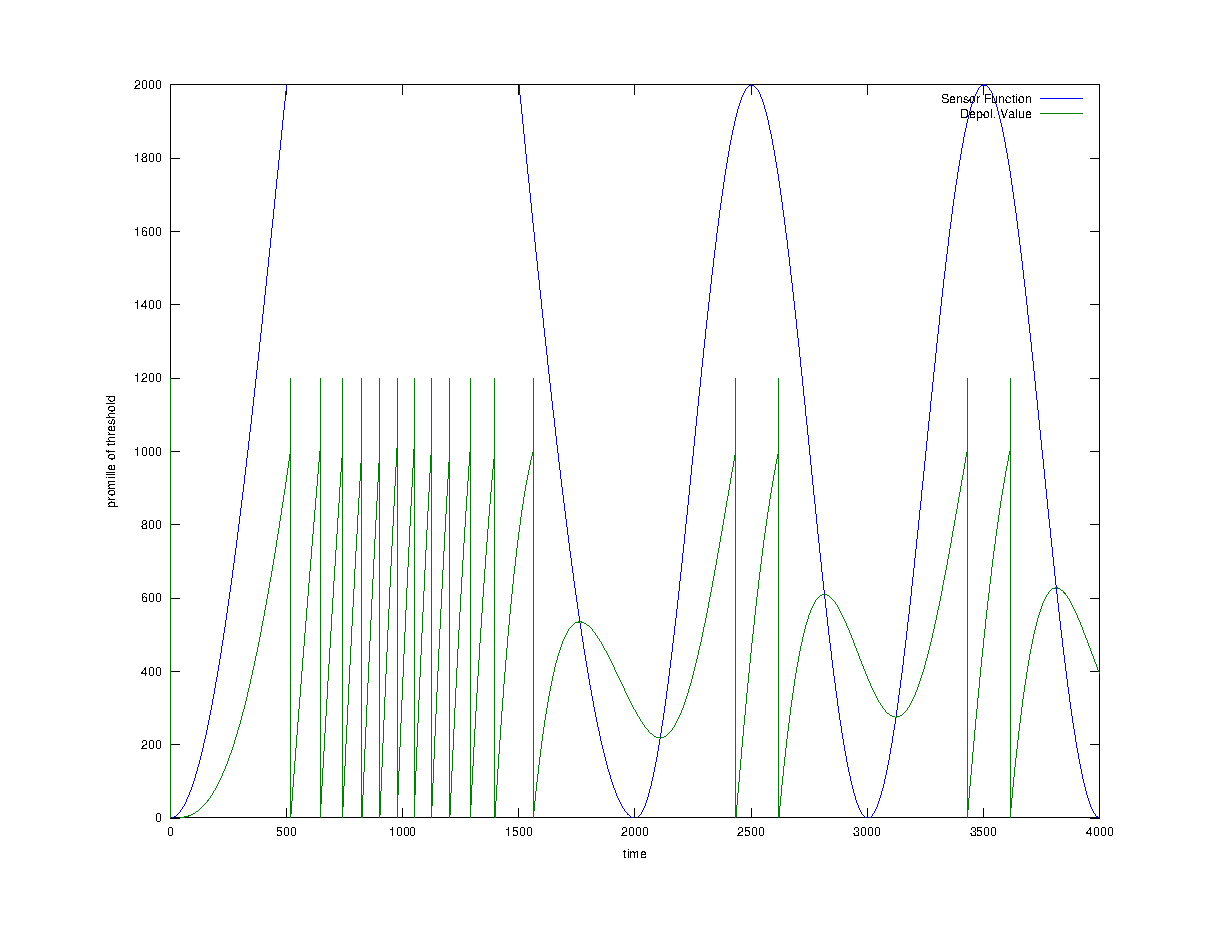
\includegraphics[width=0.95\textwidth]{sensorAuron}
	\caption{Example of the use of a sensor auron. A sensor function is designed to be \mbox{$2\tau (1-cos(\pi \frac{t}{1000}))$} before time $t=1500$. After this it halves the amplitude and doubles the frequency.
			The blue curve represents the sensor function. The green curve represents the ``depolarization'' of the node. Firing is represented by a vertical line in the value curve.
			(Generated by AuroSim)} 
	\label{figSensorAuronExample}
\end{figure}

	The sensor nodes are instances of a class named \emph{s\_sensor\_auron} for the SANN model or \emph{K\_sensor\_auron} for the $\kappa$ANN model.
	In the following text, the \emph{K\_sensor\_auron} will be introduced, but the aspects are general and the presented aspects are valid for both classes. % same goes for the SANN variant of the node.

 	The sensor auron is a specialized auron node, where the activity level of the node varies with some external function.
	This function is called ``the sensor function'', and is possible to design specifically for what is tested for the node.
	In sec. \ref{secComparisonOfMechanismsOfNodeElements} this is used;
		Functions are especially designed to compare different aspects of the SANN node vs. the $\kappa$ANN node. %between the two models.

	Objects of these classes update its activity level each time iteration.
	The activity level, represented by $\kappa$ in $\kappa$ANN, is given by the output of some ``sensor function''.

	The operation of the sensor node is very inspired by biology, where we also have specialized receptor cells responsible for the monitoring of the environment\cite{NeuroscienceExploringTheBrain3edKAP8}.

	\subsubsection{The sensor function is a function pointer}
	The sensor function is the method that ``senses''.
	This can be designed to test certain mechanism of the node.
	
	In fig. \ref{figSensorAuronExample}, this sensor function is set to be a sinusoidal curve with an amplitude of $4 \tau$. 
	At time $t=1500$, the sensor function halves the amplitute and doubles the frequency of the sinusoidal cuve.
	The figure shows the sensor function and the resulting depolarization of the sensor auron.

	The sensor auron class contain a function pointer.
\begin{lstlisting}
double (*pSensorFunction)(void);
\end{lstlisting}
	At the time of construction of each sensor auron object, the constructor takes a function pointer as an argument and assigns its function pointer variable to this value.
	This gives that for a new test case, it is possible to define a new function, and send in the reference to this function to the constructor of the sensor auron.
\begin{lstlisting}
K_sensor_auron::K_sensor_auron(
  std::string sNavn_Arg, double (*pFunk_arg)(void) ) 
     :  K_auron(sNavn_Arg)
{
	// Assign the sensor function:
	pSensorFunction = pFunk_arg;
	// Add to pAllSensorAurons list:
	pAllSensorAurons.push_back(this);

	...
}
\end{lstlisting}

	\subsubsection{Updating The Sensor Auron}
	The static variable \emph{pAllSensorAurons} is a list containing all the sensor aurons.
	After \emph{time\_class::doTask()} iterates time, all sensor aurons(listed in \emph{pAllSensorAurons}) are updated.
	Inspired by biology, the sensing done by the sensor auron happens at the dendrite;
		The sensor auron is updated by sending in the sensed signal to the dendrite's \emph{newSignal()} function.
	%The sensed signal is therefore sent in to the dendrite as the derived of the sensor function. % , before the result is sent in to the \emph{newSignal()} function.


	For the K\_sensor\_auron this gives the code
\begin{lstlisting}
inline void K_sensor_auron::updateSensorValue()
{ 
	// Use two variables, to find the derived.
	dLastSensedValue = dSensedValue;
	dSensedValue = (*pSensorFunction)(); 

	// Use the native mechanism for dendritic integration for the sensor neuron:
	if( dSensedValue != dLastSensedValue){
		changeKappa_derivedArg( dSensedValue-dLastSensedValue );
	}
}
\end{lstlisting}

	%Litt meir, kanskje. Ikkje heilt naudsynt..











%
\chapter{ Implementation  -- Denne kan kanskje takast vekk}
% Her skal eg skrive om implementasjon av det som er planlagt i "Design".
% Kvifor C++ ?


	%Innledning, kva programmeringsspråk brukes, osv. Etabler eit utgangdspunkt for resten av teksten!
	Når man implementerer for å sammenligne to modeller er det best at de to er mest mulig lik. Dette kan lett gjøres vha. arv. Peiker mot OO-språk.
	
	Det sterke fokus på være mest mulig likt biologiske neurale system peiker mot OO-språk virker bra. Da kan man dele opp neuronet i "compartments", som i utgangspunktet er adskilt.

	C er eit språk som er effektivt (raskt), samtidig som det har vore undervist på kyb.

	= C++.

	Etterkvart: Skriv litt om Stroustrup's anbefalinger om å bruke stl.




\section{Fokus}
I denne oppgaven er ikkje fokus på effektivitet av utregningene, men evt. effektivitetsdifferanse mellom de to. 
Først brukte eg integer for å beskrive f.eks. depol. og Kappa, men dette førte til en del avrundingsfeil. 
Gjekk dermed over til å bruke flyttal for å beskrive aktivitetsvariabel. (denne notaten er notert før eg har endra de fra int til float.. Sjå korleis det går.



\section{Notater:}
\subsection{Skruve om std::vector vs. list.}
Eg har brukt en halv dag på å teste om eg skal bruke vector eller list for pAllAurons og pAllKappaAurons. Konskluderte med at det ikkje hadde noko å seie.

Hadde 101 test-auron (K\_auron) og eit sensor-auron. De var ikkje kobla ihop, og hadde kvar en Kappa på 2.07*FYRINGSTERSKEL. Sensorauronet hadde en sinus-varierende kappa.
Kjørte 10.000 tidsiterasjoner. Resultat av kjøretid:

Vector variant:
15.626 15,537 14,8 13,3 13,5 13,6

List variant:
13,46 13,41 	13,72 13,6 14,9 14,7 13,3 14,9

Konkluderer med at de ikkje har stor nok forskjell til å bry seg.

(dette kan være smart å skrive inn i rapporten. (og da blir ikkje denne halve dagen fullstendig bortkasta..))

 TODO Sjå gjennom implementasjon.tex, og sjå kva som skal flyttast inn i implementasjon_[K/S]ANN.tex eller design.tex

%TODO Denne må skrives heil om: Sett av en dag til dette

%Eg forstår kvifor SANN ikkje har asynkron tid. For alle element må man kvar iterasjon gjennomføre lekkasje. Dette er brute-force måte å gjøre det på. Bedre er å bruke pow() eller løkker får den får innput gjennom synapse.
%Men det intuitive er å kjøre brute-force lekkasje kvar iterasjon. Bedre paralellisering om det gjøres alt på en gang. Gjør det slik, og skriv om kvifor!
%
%Hugs også at eg har laga arbeidskø av class tidsInterface, og alle som skal schedules er arvinger av denne. Dette gjør at det er mulig å simulere time-delay i synapse-overføring, axon-overføring, axon-hillock-AP-initiering, osv.





%*********************** SANN ***************************
%\chapter{Implementasjon: SANN}



%TODO Sjå design.tex (mot slutten er eit parti som er utkommentert som bestkrive s\_dendrite sin funksjon sammen med i_dendrite)





\section{SANN --- Design and Implementation}
\label{secSANN} 


	% Kjør masse sitering eller referering innad i dokumentet for å hente ut meir poeng fra sensor.
	% Skrive at "Alle SANN" istedenfor "the usual way ..". Det er litt vanskelig å skrive "alle" uten å være påståelig.
	% Ikkje skriv "usual way". Skriv heller at det er implementert som .. ( i dette prosjektet.. ). Skrive så at modellen SANN tilseier at dette er metoden..
	The usual way to implement spiking artificial neural networks (SANN) is a direct simulation of the mechanisms that generate the behaviour of the neuron.
	
	In terminology from graph teory, a neural netwoks is a directed cyclic graph with a dynamic amplification (weights) on its edges.
	The nodes of this graph are the neurons and the edges are the synapses between two neurons.% (The connection between them).

	In neural networks you have synaptic plasticity, or change of the weights of the edges. Synaptic plasticity is what is referred to as learning in neuroscience. %TODO ref bear eller noke.


	Earlier ANNs can be said to be a set of nodes that transmits continuous variables through its output synapses. The timing of such networks is synchrounous, and the transmission of each node is governed by a central clock.
	For networks of biologic neurons, the transmission is completely asynchronous, an the transmission happens whenever the neuron depolarization reaches the firing threshold.
	The value is increased or decreased by excitatory or inhibitory synaptic input, respectably .
	
	% Ny tanke: synaptisk plastisitet er kanskje større innerst på axonet: her er kanskje AP litt større, så når dette ganges inn med synaptisk effektivitet for å finne 'synaptic weight' vil dette gi at små endringer vil gi større utfall
	% 	for synapser som ligger tidlig på axonet. Dette er logisk dersom størrelsen på AP varierer.
	When the value of the node reaches the firing threshold for the neuron we get transmission through its output synapses.
	%When the value of the SN reaches the firing threshold, an action potantial is transmitted by letting the synapse add its weight to the postsynaptic neuron.
	As the action potential is seen as a boolean signal internally in the neuron, we get a constant depolarization on all the output synapses of a neuron.
	This depolarization gives the amount of neurotransmitter release. 
	Because this depolarization is constant over time, we can include this aspect into the synaptic weight of the edge, $W_{ij}$.
	In this simulation we simplify the transmission, and other effects of elements like pre--action potential depolarization of the synapse is not included.%XXX FORENKLA VEKK
	We then get that synaptic transmission can be executed by simply adding the synaptic weight to the postsynaptic neurons value.
	%SKrive at dette er vanlig, og at dersom det er ønskelig å innføre slike prinsipp, kan dette lett gjøres pga den modulære oppbygginga til simuleringa.
	The modular design of this implementation makes it possible to make changes to the indivitual elements without affecting the whole implementation.
	It is therefore not much work to implement elements such as short term plasticity and axo--axonic synapses in future uses of this simulator.
	% Forrige linja har kanskje ikkje så mykje med oppgava å gjøre?

	% Kanskje bare: "The neuron .."
	%The nodes of ANN are
	The neuron is often modelled as a leaky--integrate--and--fire neuron (LIF-neuron). %TODO Referer.
	In this model the node ``leaks'' a certain amount of the potential, and the value decreases a over time. 
	% Skrive om ekvivalent kondensatorkrets?
	This value varies as a function of the value of the neuron, and we get a first order differential equation for the value of the node.
	For SANN nodes (SN) this is implemented as subtracting a product of the value every time iteration. 
	\begin{equation}
	v_t = v_{t-1} - v_{t-1}  \alpha % = (1-\alpha)  v_{t-1} Skal skrive egen section om dette. Sparer den siste godbiten..
	\end{equation}
	The leakage of value will be further discussed in section \ref{secTheLeakageForSANN}.

	Because every aspect that is thought important in neural signalling is simulated in SANN, 
		we can say that this is a direct simulation of each node of the network.   % KVA MEINER EG med direct manner? --At kvar ting er simulert kvart tidssteg. Naiv implementasjon. Ueffektivt!
	% Skriv kva eg meiner med "direct simulation". (at kvart elmement som er viktig simuleres for seg selv, kvart tidssteg. Nain implementasjon).
	%The simulation of the mechanisms of the nodes is 
	

	\subsection{The Nodes' Input}
	In this implementation, all transmissions through the input synapses arrive at the dendrite.
	Here the membrane potential is either increased or decreased, depending on whether the synapse is an excitatory og inhibitory synapse.

	Whenever the membrane potential goes to suprathreshold levels (value goes above the predefined firing threshold), an action potential is simulated.
	%When the membrane potential of the axon is higher than the firing threshold, specialized voltage gated channels are opened, and we get the self--carrying action potential. 
	As the biological acion potential initiates transmission in all the neuron's output synapses, the simulated action potential will after a delay initiate the ANN's version of a synaptic transmission.
	For a review of the biological action potential, it is referred to section \ref{ssecTheActionPotential}. %XXX Veit ikkje heilt korleis eg skal skrive : "gå tilbake til start (section ?? )".
	%Se section \ref{ssecTheActionPotential} for a description of the action potential in the biological neuron.
	
	% TODO Neste linja stater for svakt. Dersom det er debatert er det lite truleg. Framstill det som at dette ikkje er debattert (det er ikkje det. (?))
	%Another mechanism that is debated in the neuroscience community is the possibility of some intracellular signalling mechanism that will initiate the action potential.% at the axon hillock. %TODO referer!
	%This mechanism is initiated by a suprathreshold potentiation somewhere on the dendrite, sendt through the cytoplasm of the neuron to the axon hillock, where it will cause the initiation of an action potential.

	As synaptic input is defined to arrive at the dendrite in the emulated neuron, the dendrite is responsible for the action of recieving the transmission.
	This is done by the function \emph{s\_dendrite::newInputSignal(double)}.
	%As the function is inherited from \emph{i\_dendrite}, where it is defined as a pure virtual funtion, the function must be declared in class \emph{s\_dendrite}. XXX XXX XXX XXX Kjempeviktig poeng for "comparison"
	

	In the biological neuron, a new input signal changes the value of the postsynaptic neuron propotionally with the size of the transmission.
	The size of the transmission is given by the synaptic weigth $w_{ij}$.
	When a new transmission comes through a synapse, it is therefore the synaptic weigth that is sent into the postsynaptic dendrite.
	Because future use of the code may include short--term synaptic plasticity, or other aspects changing the size of the transmission from the synapse, the size of the transmission is sent in as an argument to the postsynaptic dendrite.
	% TODO Gjør setninga over lettare! =kortare!
	%As the size of transmission is given by the strength of the connection, the synaptic weight $w_{ij}$, the synaptic weight is what is sent in from the synapse.
	%Because of future use of the code may have short--term synaptic plasticity, the size of the transmission is sendt to the postsynaptic dendrite as an argument (se appendix \ref{appendixSynPlast} for a review of synaptic plasticity).



%UNDER: FEIL FOKUS, dette er ikkje biologi-kap.!
%	A dendritic input will change the electrical potential of the cytoplasm comparet to the extracellular fluid. This electrochemical potential will propagate with a small time delay through the cell body, to the axon hillock.
%	% Skriv at det også kan være andre time delays. Eg (og stavdahl) ser ikkje på strøm som treigt..
%	In this implementation, the time delay is implemented by having a small delay of one time iteration before initiating the action potential.
%	This is done by the mechanisms of the pWorkTaskQue (se section \ref{ssecTime} for more about pWorkTaskQue).% and section \ref{ssecSANNAP}).
%

	\subsection{The ``Leakage''}
	\label{secTheLeakageForSANN}
	%TODO Skriv i introen til section: om lekkasjen. Skriv om LIF. Internreferer!

	The LIF neuron is modelled as being leaky with respects to time. %TODO REFERER.
	One way of simulating leakage is to update the value every time iteration. %eller recalculate?
	The leak can be defined as a value propotional to last calculated value.
	As this is the value from the last time iteration, we get the equation for the new value $v_t$
	
	\begin{equation}
		v_t = v_{t-1} - \alpha v_{t-1} \; = (1-\alpha) \cdot v_{t-1}
		\label{eqOppdateringAvVerdiEtterLekkasjeSimpelVariant}
	\end{equation}

	As we are concerned with efficiancy in the simulation, recaluclating the value for each node every time iteration is not preferable.
%
	The time design introduced in sec. \ref{ssecTime} enables the implementation to be an event--driven simulation of the neuron;
		The value of the node is only updated when the value is to be changed of othervise used.
	%For this implementation, the time design enables us to have an event based simulation of the neuron.
	%The value of each node is only updated when the value is changed or othervise used.
	%This involves that the node is updated only when the value is changed.

	From eq. \eqref{eqOppdateringAvVerdiEtterLekkasjeSimpelVariant} it can be shown that 

	\begin{equation}
		v_t = v_{t-x} (1-\alpha)^{t-x}
		\label{eqLeakageForSANN}
	\end{equation}
	
	Where $x$ is the time iteration when the value was last updated.
	%Where $l$ is the last time iteration the value was updated.
	Because leakage is a diminishing mechanism for the value of the node, the value will not go above firing threshold as a consequence of leakage alone.
	This makes it safe to update the value only when the value is used.


	For an event--driven calculation scheme, the calculation of leakage could be made more effective by updating the value by eq. \eqref{eqLeakageForSANN}. %, only when the node's value is used.
	%In this case we can make the calculation of leakage more effective by updating the value only when it is used.
%	
%	Where $n$ is the last time where the value was updated. 
%	Because leakage is a diminishing effect on the value, the value will not go above the firing threshold because of this effect alone.
%	This makes it entirely safe to use \eqref{eqLeakageForSANN} in the implementation of SANN.

% todo? Her kan eg lage eit plott av auron1 som lekker kvar iterasjon og auron2 som venter 30 iterasjoner før den lekke. Desse vil ligge over kvarandre.
% Lag auron1-plott med .-plott og auron2 som @-plott. (sjå s_dendrite::calulateLeakage() : kommentaren seier at eg allerede har gjort forsøket. Funka fett.)

\begin{lstlisting}
inline void s_dendrite::calculateLeakage()
{ 
	// Calulates new value for the node
	pElementOfAuron->dAktivitetsVariabel *= pow((double)(1-ALPHA), 
						(double)(time_class::getTid() - 
						 pElementOfAuron->ulTimestampLastInput) );
}
\end{lstlisting}

	The leakage is calculated whenever the node gets a new input, or the value is used.
	E.g. when the 
	The leakage will be calculated every time the value of the node is used or changed.
	This means that whenever the dendrite gets a new transmission from one of its input synapses, \emph{s\_dendrite::calculateLeakage()} is called.








	\subsection{Action Potential in SANN}
	\label{ssecSANNAP}
	When the depolarisasjon of the membrane goes above the firing threshold, the s\_auron element of the node is inserted into pWorkTaskQue.
	This simulates the delay of the intracellular signal propagation, causing a small time delay before calling \emph{s\_auron::doTask()}.
	In this context, \emph{s\_auron} have the role of the axon hillock.
	As the axon hillock initiates the action potential for the biological system, the \emph{s\_auron} starts the simulated action potential by inserting a pointer to the node's \emph{s\_axon} object into \emph{pWorkTaskQue}.

	After the delay caused by the simulated action potential, the axon segment's \emph{s\_axon::doTask()} is executed.
	%After the axon's time delay (depending on the number of serial axon segments), the axon segment's \emph{s\_axon::doTask()} is called, 
	%The next time iteration, the node's \emph{s\_axon::doTask()} will be called,
	This function inserts all the segment's output synapses into \emph{pWorkTaskQue}.

	Multiple axon segment in series cause an increased time delay.
	%If we have multiple axon elements in series, this time delay is increased. 
	If we also decrease the step size of the simulation, we get an increased spatiotemporal resolution.
	By this expression it is referred to the fact that the intracellular tranmission does not happen instantaneously, and that the travelling distance gives the time of the transmission.
	With multiple axon elements in series, we could therefore separate the output synapses to different groups based on their location.
	The different groups of synapses would then be given different time delays based on their distance along the axon.

	%This time delay can be increased by having multible s\_axon elements in series, but for the initial testing of this simulator, one single axon segment was used to model the axon.
	In AuroSim, the focus for implementation is a pragmatic focus, in addition to compare the two models. 
	The comparison will only suffer if we make each implementation overly complex.
	For these reasons, the axon is implemented as a single axon segment containing all the node's output synapses.

	When the ``action potential'' reaches the synapses, these synapses are inserted into \emph{pWorkTaskQue}.
	The delay of one iteration corresponds to the delay of a synaptic tranmission.
	This delay is probably way to small compared to the biological system, as a synaptic tranmission consists of the release of neurotransmitters(NT), 
		diffusing of NT through the synaptic cleft and activation of postsynaptic receptors\cite{PurvesNeuroscienceKAP05}
	The transmission thought a synapse is a simplification anyway, and we will not follow this any further. %TODO Skriv om. Begynner å bli trøtt.

	%Also the output synapses of the node will be executed by adding a pointer to the element to pWorkTaskQue.
	%The delay here corresponds to the time delay of a synaptic transmission, due to the delay caused by the release of neurotransmittors(NT), diffusing of NT through the synaptic cleft and the activation of the postsynaptic receptors.
	% % TODO Referer internt til BiologiskeSystemet.tex (Men først skriv om dette). Kanskje bedre å bare skrive om det der, og referere dit (skrive bare "corresponds to the delay of syn.transmission" (med ref. til bioSys) her..)
	%After the time delay, the output synapse's \emph{s\_synapse::doTask()} will be executed, causing the excitation or inhibition of the postsynaptic node to each of the node's output synapse. 
	% %, depending of the nature of each synapse (whether it is excitatory or inhibitory).
	
	The simulated synaptic tranmission is executed by the output synapse's \emph{doTask()} function.
	This gives an increases or decreases the postsynaptic node's value, depending on whether it is an excitatory or inhibitory synapse.
	The size of the transmission is given by the synaptic weight.
	%This is done by sending the new signal to the postsynaptic dendrite's input function \emph{newInputSignal(double)}.

	%As an input is presented to the postsynaptic dendrite, an argument is sent in to the function \emph{s\_dendrite::newInputSignal(double)}.
	A new input signal is presented to the postsynaptic dendrite by sending in the synaptic weight to the function \emph{s\_dendrite::newInputSignal(double)}.
	Synaptic transmission is thus divided into two parts, where the postsynaptic dendrite ultimately controls the change of depolarisasjon for the postsynaptic node.
	The postsynaptic depolarisasjon is changed by an amount given by the argument presented, and by the predefined time constant of the node.
	After an incoming transmission the postsynaptic node is change by a value of $\pm \frac{W_{ij}}{\alpha}$, depending on the nature of the synapse.
%	The postsynaptic potential will change as a function of the synaptic weight. For this simulation the postsynaptic potential will change with a factor $\frac{1}{\alpha}$. %XXX Kvifor? 1/a. Sjekk regtek bok.
%	This is handled in the postsynaptic dendrite, causing the postsynaptic depolarisasjon to change by $\pm \frac{W_{ij}}{\alpha}$, depending on the nature of the synapse.

	%TODO TODO OTOD TODO SKRIV OM dale's principle I BiologiskeSystemet.tex TODO TODO Og referer dit.
	In many ANNs the synapse has the ability to change between between being excitatory and inhibitory. 
	This corresponds to e.g. a positive synaptic weight becoming negative after synaptic plasticity.
	According to Dale's Principle, neurons release one neurotransmittor\cite{NeuroscienceExploringTheBrain3edKAP6}
%	The result of this is that in biology, synapses are either excitatory or inhibitory.

	A result of this is that synapses can hardly ``change its nature'' and go from being excitatory to being inhibitory, and vice versa.
	%Synapses can not go from being excitatory to being inhibitory, and vice versa.
	In this simulation, excitatory and inhibitory synapses are therefore separated by a boolean \emph{bInhibitoryEffect}. 
	The transmission is implemented in \emph{s\_synapse::doTask()} as
\begin{lstlisting}
inline void s_synapse::doTask()
{
  pPostNodeDendrite->newInputSignal( 
    (1-2*bInhibitoryEffect) * dSynapticWeight );
}
\end{lstlisting}

	When synaptic plasticity is implemented for this simulation, it is important to make shure that the synaptic weight does not become negative. 
%	The specific mechanisms of synaptic plasticity have not been designed, but when the synaptic weight comes to close to being zero, the biological synapse will dissapear.
% 	The plan is to make some condition for the dissapation of synapses as the synaptic weight becomes to small.

\subsection{The Response of the SN}
	In the previous sections, the design of each node for the SANN was introduced.
	The activity variable for the SN corresponds to the level of depolarization of the membrane potential for the biological neuron.
	Excitatory synaptic input to a node will increase the value of the node and inhibitory synaptic input will decrease the node's value.

	\begin{figure}[hb!tp]
		\centering 		
		\includegraphics[width=0.65\textwidth]{depolPlotAvSN/auronE_fig.jpg}
		\caption{``Neural oscillator'': test circuit for SANN. Auron A[1-9] is connected with a synaptic weight $w_{ij}=1$, causing firing by a single transmission. 
		All aurons in the neural oscillator exept node A7 is connected to auronE.
		}
		\label{figAuronE_schematics}
	\end{figure}

	Each time iteration, the value of the node will diminish due to ``leakage''. 
	In AuroSim, the leakage is only computed whenever the value is used.
	This is done by the use of equation \eqref{eqLeakageForSANN}.

	%Skriv først (underveis i neste avsnitt) at for å teste dette kan vi lage en "neural oscillator", en krets som vil holdes aktiv av seg selv. Kvar output .. osv...
	To test the implementation of the SN, the circuit in fig. \ref{figAuronE_schematics}
		was tested. The connections between node A1 and node A2 has a synaptic weight of weight $W_{21}=1.1$, large enough to excite node A2 above firing threshold in a single transmission.
	Each of the nodes A1-A9 has a synapse to the next node with a synaptic weight of one. 
	From node A9, there is a synapse to node A1 of weitht 1 completing the ``neural oscillator''. In this circuit each of the nodes will fire once every ninth time iteration.

	%TODO Lag figur om kretsen. Den skal ligge her. Neste plott er resultatet, og kan komme på neste side, eller noke..
	\begin{figure}[hb!tp]
		\centering 				%TODO TODO Flytt dette plottet ned, ca ei side. Putt fig. av oppsett, her.
		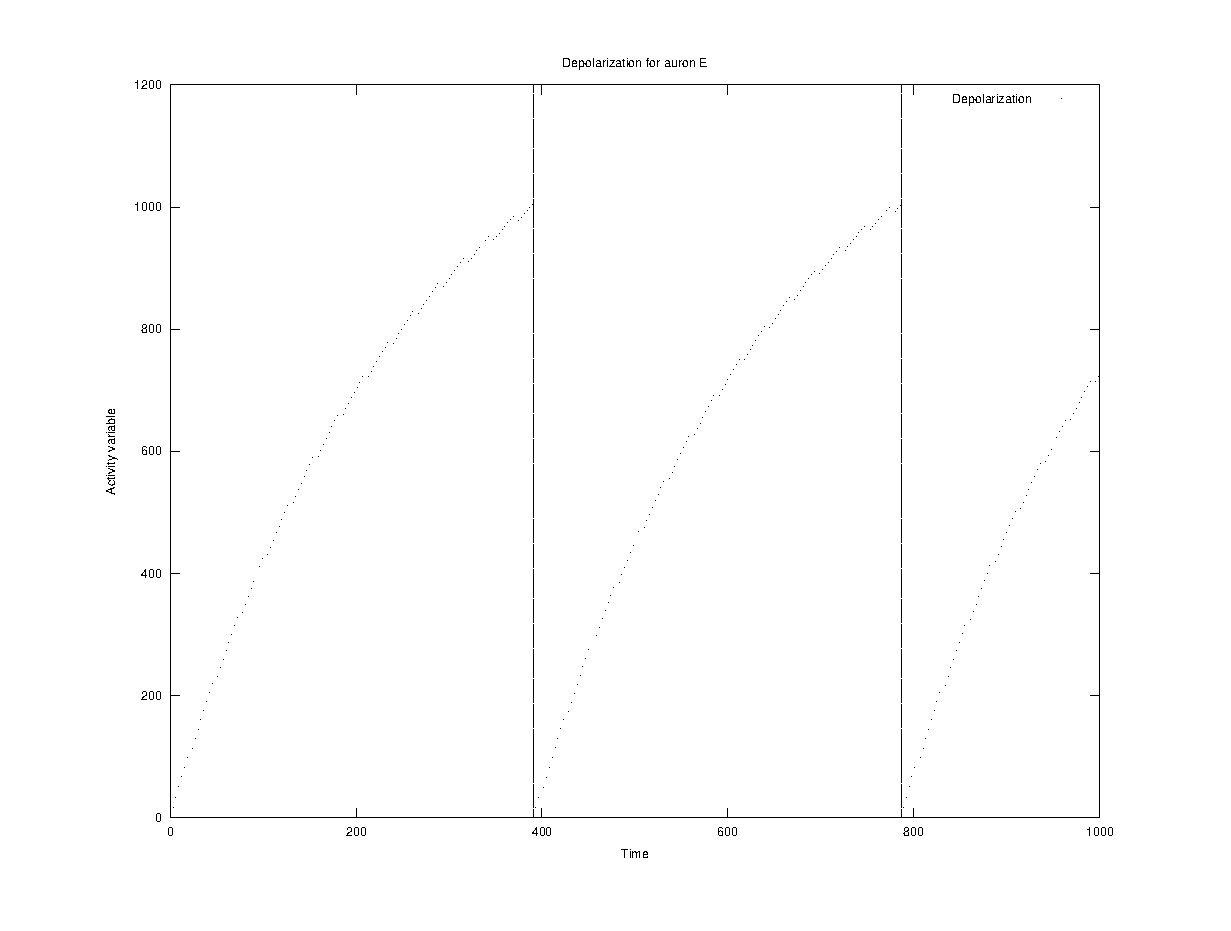
\includegraphics[width=0.95\textwidth]{depolPlotAvSN/eps_auronE-depol}
		\caption{Depolarization plot for auronE in the neural circuit from fig ?. The activity variable for a SN corresponds to the depolarization of a neuron.
		(Generated by AuroSim)} %TODO TODO Lag plot som beskriver kretsen, og referer dit, her.
		\label{figAuronE}
	\end{figure}

	Except from node A7, every node in the ``neural oscillator'' have a synaptic connection to node E with a synaptic weight $W_{Ej}=0.017$ . %todo: ta vekk "constant" ?
	There is no synapse from A7 to node E.
	%From each of the nodes in the ``neural oscillator'' except for node A7, there is a synaptic connection to node E with a constant synaptic weight $W_{Ej}=0.0017$ .
	In the course of one period of the oscillator we get eight excitatory inputs to node E, each transmission of size $W_{Ej}*\tau = 17$. 
	Every ninth time iteration we get no input to node E.

	Fig. \ref{figAuronE} shows the resulting depolarization plot of node E. 
	% TODO flytt neste linja litt ned (eller noke, passer ikkje akkurat her..)
	%Fig.\ref{figAuronE} is a direct result of the execution of the log files created by the simulator.
	This plot is the result of running the octave log script of auron E in octave after the execution of AuronSim.
	%

	We can see that node E gets a steady input from the nodes of the ``neural oscillator''.
	%
	Every cycle of the oscillator there is a pause in the excitatory input to node E, resulting in a small drop in node E's activity variable. 
	One cycle of the oscillator is represented by 8 entries in the log file, one log entry after each transmission.
	This can also be observed in fig. \ref{figAuronE} by remembering that during a pause in transmission, the change of value for the node is only due to the ``leakage'' of the node's value.
	Every 8'th value of node E's value is smaller than the previous entry due to this effect.
	%This is due to the absense of excitatory input and due to the leakage during the pause in excitatory input to the node.

	%After the pause in synaptic input to node E, the leakage is calculated at the time of the next transmission by eq. \eqref{eqLeakageForSANN}, resulting in the little drop in the node's value.

	% TODO Skriv det under i "log-file"-biden av design.tex! Passer ikkje her...
	%The constructor of every node creates a log file and each time the nodes activity variable is changed, the time iteration and the new value is written to the log file.
	%The destruction of each node finalize the node's log file, by writing octave calls that makes plots like the one in fig. \ref{figAuronE} and prints the resulting plot to an eps file.
	%Many of the eps files included in this report comes from the execution of similar octave script--file logs.

	We can also see that the mechanisms behind firing an action potential works. 
	%When the value of the node goes over the firing threshold an action potential is fired.  %XXX Dette er kanskje bedre måte å sei det enn neste?
	When the node's value goes to suprathreshold levels, an action potential is fired. %Skriv: dette er representert ved en vertikal strek i figuren (eller i logg-plottet).
	In fig. \ref{figAuronE} we can see that the node's value is reset to zero after firing an action potential.
	%TODO Ta med det neste, men ikkje før eg er heilt sikker, og kan gjøre det til meir enn en påstand (ta med noke i appendix, eller skrive tidspunkt for de to)
	%In the corresponding log file for the synaptic transmission of node E's output synapses, it can be observed that the synaptic transmission comes two time iterations after the node's value reaches the firing threshold. 
	%%Similar plots of the synaptic transmission from the synapses log file shows transmission after the time delay caused by the initiation of an action potential and the delay caused by the action potential propagating through the axon.
	%TODO Være sikker på at det er har skrevet her er heilt rett. (flaut dersom det er en åpenbar feil, her!)
	Analysis of the log files shows that node E fires one action potential at time 391 and one at time 787.
	The synapse's log file shows transmission at time 393 and 789, each at two time steps after node E's value goes above firing threshold.
	%each transmission at two time iterations after node E's value goes above the firing threshold. 
	This tells us that the simulated delay caused by the action potential initiation and propagation works as designed.
	% Auron E: AP    på tid: 391 og 787
	% Syn overføring på tid: 393 og 789
	
	The log entry for the next time iteration is zero, due to the simulated refraction period of the node.
	Two time iterations after the action potential the node's value becomes or 17. %TODO? Skal eg skrive litt om at eg kjører størrelse på W_ij i kor mykje postsyn. går mot fyring. I promille? Viktig poeng!
	%Har sjekka: Dette gjelder for begge overføringene/AP i simuleringen. Skriv dette, og at det betyr at vi for desse to overføingene faller "pause" ikkje til to tidssteg etter fyring.
	%This corresponds to the defined synaptic transmission for each of the synpses of the circuit. %Kanskje heller : ".. for the synapse in question"? ELLER at dette betyr at i desse tilfellene har vi ikkje pause på dette tidspunktet.
	This corresponds to a transmission through one of the synpses.
	As AuroSim does not calculate synaptic plasticity, the result of a transmission is a constant postsynaptic change of size 18.

	%This analysis shows that the above discussed design of the simulated neuron gives us the mechanisms of the neuron, in respect to synaptic transmission, leakage, refraction time and action potential firing.
	This analysis shows that, in respect to synaptic transmission, leaky integration, refraction time and action potential firing, the design and implementation gives the behaviour of the neuron model used. 
																																														  %ELLER: .. considered model of the neuron.





% Feil ved denne forenklinga:
%  - vi går ut fra at verdien ikkje lekker mellom dendrite og axon hillock. Dette er nok litt feil, men ikkje mykje.
% 	Dersom vi hadde hatt dette, måtte vi implementert lekkasjen, men også en liten time delay før verdien blir lagt til verdien i axon hillock. Dette er computationally ineffektivt.
% 	Dersom dette skal implementeres (at programmet skal være en simulering av neurale system, så er dette mulig ved å ha en egen node for axon hillock)
%  - vi går ut fra at synaptic transmission gir total overføring i.l.a. ei overførin. Dette er nok feil.
	
	
	%TODO Skriv korleis dette kan gjøres for KN.

	% Lag diagram om korleis dette funker. Kanskje eit "uml-signal diagram"?   (Treng fleire figurer her!)

	% TODO Lag en figur som viser oppsettet til kretsen.









% (Neste som kommer er KANN--implemenasjon-kapittelet)

%
% PLAN:
% - ta med "propagating of kappa". At metoden brukt er antagelig ikkje den mest effektive, men det gjøres likt for å lage det meir egna for sammenligning.(ligger i implementation.tex)
% - ta med "om oppsamling av kappa" (ligger i implementation.tex)

% Kan sei at dette er "original work by the author." Dette kan ivertfall brukes når dette kapittel blir referert til!

%TODO Skriv om mealy automata, ANN, input som aktivitetsvariabel for 1.gen. og 2.gen. ANN og state som aktivitetsvariabel for 3.gen. ANN.
% 	Kan da skrive at denne modellen har aktivitetsvariabel for både state og input (Kappa, dDepolAtStartOfTimeWindow), og kan dermed lett transformerer KANN's aktivitetsvariabel over til 1g.ANN, 2g.ANN og 3g.ANN!
% 	Sjå [ ref_asdf2143@ANN ] i ANN.tex.

%*********************** KANN ***************************
\chapter{implementasjon: KANN}
	Skriv først innledning, med mål om å sette meg og leser på samme utgangsnivå.
	Skrive litt om kvifor eg tenker det er lurt å gå videre fra SANN.
	Modellere det, og bruke formalisert matematikk fremfor å ha ei naiv direkte simulering av mekanismene i enkeltneuronet.
	%Skrive at eg desverre ikkje fekk tid til syn.P. i dette prosjektet?

	Skriv også det som står i TODO over, eller i ANN.tex: [ ref\_asdf2143@ANN ]% Søk etter ref_asdf2143@ANN i fila ANN.tex.
	"As we will see, this new model for ANN have both a state and output given by the last time iteration's state and the input to the node. 
	This gives that the node is able to communicate with all the previous forms of ANN, and might serve as an important transform between different models of ANN."
	%XXX Dette er vel heller analyse, forresten. TODO Skriv det over i analyse/comparison kapittel.
	% MEN kanskje også her?

	
	\section{Updating $\kappa$} %Calculation and recalculation of $\kappa$
		\subsection{Synaptic transmission}
			% skrive om korleis synaptic transmission fåregår (generellt (om at $\kappa_{ij} = \frac{W_{ij}}{p_{pre}}$ ).
			In biology, a synaptic transmission happens every time a presynaptic action potential is fired.
			The size of this transmission is given by the synaptic weight of the synapse.

			Over some time interval, the total transmisson in a synapse ,$o(\Delta t)$, can be modelled as the synaptic weight times the presynaptic neurons firing frequency times the evaluated time interval.
			We write the presynaptic firing frequency as $f_{pre} = \frac{1}{p_{pre}} = \frac{1}{p(\kappa_{pre})}$ and get:
			\begin{equation}
				\label{eqSynapticTransmission}
				o(\Delta t) = \frac{ W_{ij} }{ p(\kappa_{pre})} * \Delta t 
			\end{equation}

			In discrete--time systems, we can define every synaptic transmission to last for one time iteration (if the time step is large enough).  % MED ELLER IKKJE: "(if the time step is large enough)" ??? XXX
			This causes $\Delta t$ to become constant. We can incoorporate this constant into $W_{ij}$.

			For an ANN based on the activity variable $\kappa$, as previously introduced in chapter \ref{secMatematiskModelleringAvBioNeuron} %TODO Sjekk denne  referansen bedre / skriv bedre (?).
			eq. \eqref{eqSynapticTransmission} is highly relevant.  % highly relevant skurrer litt. Det er veldig relevant. Finn synonym..
			If we define $\Delta t$ to be some constant, and incoorporate this constant into $W_{ij}$, we get the equation for the synaptic transmission of the activity variable.
			We call the size of this transmission $\kappa_{ij}$.

			\begin{equation}
				\label{eqSynapticTransmissionForKANN}
				\kappa_{ij} = \frac{ W_{ij} }{ p(\kappa_{pre})}
			\end{equation}

			For nodes with multiple input synapses, the activity variable $\kappa$ is the sum of all the contributions from different synapses. %VERIFISER DETTE! Vær heilt heilt sikker på at K=sum(K_ij)
			We can write this mathematically as 
			\begin{equation}
				\label{eqSumOfKij}
				\kappa_i = \sum_j{\kappa_{ij}}
			\end{equation}

			In this way the synaptic transmission of the individual synapses can be decoupled from the postsynaptic activity variable, $\kappa_i$.
			
		\subsection{Synaptic input to a node}
			\label{ssecSynInputToANode}
			In $\kappa$ANN we call the nodes for a K\_auron.
			The synaptic input for the activity variable of a K\_auron is defined by \eqref{eqSumOfKij}.
			%To avoid having to recalculate $\kappa_i$ from \eqref{eqSumOfKij} every time the transmission of a synapse changes, we can implement synaptic transmission as the transmission of the derived of $\kappa_{ij}$.
			To avoid recalculation of $\kappa_i$ from all the input synapses when one synapse changes its transmission, this implementation defines edge transmission as the derived of $\kappa_{ij}$.
			Now the postsynaptic $\kappa_i$ can be calculated without summing all the synapse inputs after changed input at one of its edges.
			%In this case the postsynaptic $\kappa$ can be recalucated without summing all the synaptic inputs every time one synapse changes its transmission.

			For synapses transmitting the derived of $\kappa_{ij}$ we only have to integrate this change of transmission from all the input synapses with a changed level of transmission, and get
			\begin{equation}
				\kappa_i = \sum_k{\kappa_{ik}}
			\end{equation}
			Where ${k}$ is a subset of ${j}$ consisting of all the synapses with a changed level of transmission.
			%In the case of only one synapse changing its transmission

			We can, in other words add the change in synaptic transmission, $\Delta K_{ij}$, to the postsynaptic activity variable to get the updated activity variable, $\kappa_i$.
			This can be done at the time of each transmission, and without having to consider any of the other synaptic transmissions to the node.
			
			%XX Skal eg skrive dette her:
			%If we wait until after the current time iteration before calculating the effects of the changed kappa, much calculations will be saved.

			\subsubsection{Effects of the new $\kappa$}
			When $\kappa_i$ changes for a node, we need to recalculate the inverse of the period for this new $\kappa_i$ to get the synaptic transmissions right.
			Because the time step of one time iteration is defined as the smallest time interval in the simulated system, we can define that the propagation of $\kappa$ will happen at the end of the current time iteration. %after this time interval.
			%eller "not instantly".
			Now %If we introduce this as a rule,
			 we can wait until after the current time iteration before calculating the effects of the changed $\kappa_i$.
			%The period of the node, and thus the synaptic transmission of its synapses can in this case wait to after the current time iteration before calculating the effect of the new $\kappa_i$.
			This includes recalculating the estimated firing time, the period inverse and thus the synaptic transmission, and initiate the new time window by calculating the initial depolarization of the neuron and setting 
				ulStartOfTimeWindow for the next time window.

			If we wait til after the current time iteration before calculating the effect of the changed kappa, the above calculations can be done once per time iteration instead of once for each input to the node.
																													% Og vil auke effektiviteten stort!
			This can be wieved as a time delay in the neuron, and is probably  very short compared to what it should be. % TODO: Skriv i Discussion: 
															%At denne delayen er antaklig alt for liten. Dersom eg hadde tid ville eg utforska kor lang denne delayen burde være.
															% Veldig vanskelig å vita kva den SKAL være...


			To wait with the recalculation of the variabled affected by the change in $\kappa$, is implemented with the concept of pCalculateTaskQue, introduced in section \ref{secCalcultaionTaskQue}.
			When a nodes $\kappa$ changes value, a pointer to the node is inserted into a specialized que for this use, pCalculateTaskQue.
\begin{lstlisting}
static std::list<timeInterface*> pCalculateTaskQue;
\end{lstlisting}
			This list is static in the time\_class, that is only one variable is made for time\_class (not one per object).
			When time\_class::doTask() runs, it first calls time\_class::doCalculations().
			%First it makes shure that each entry of the list pCalculateTaskQue is unique (it removes any duplicate). 

			The first task of time\_class::doCalculation() is to enshure that each element of pCalculateTaskQue is unique. 
			This is done by iterating through the list and removing all duplicates of each entry.
			
			The next task is to call each of the remaining elements' .doCalculation() function.
			The function doCalculation() is defined as a pure virtual function in timeInterface, and every class that does not define its own doCalculation() remains an interface class.
			This makes shure that every object of a timeInterface derived class have defined a doCalculation() function. This function is defined in the class if to make it possible to make an istance of the class.
			% gitt av kva elementet har behov for å vente med å kalkulere. For K_auron er det effekten av endring av Kappa som er hensiktsmessig å vente med. For s_auron er det kanskje lekkasjen?

			For K\_aurons, the inherited virtual function .doCalculation() has the task of calculating every variable that changes as a consequence of a changed activity variable for the auron.
			% TODO Skriv bedre XXX

			\subsection{Analysis of synaptic transmission as the derived}
			When synaptic transmission is defined as the derived of $\kappa_{ij}$ the gain in efficiency can be noticable. 
			It also introduces some effects that is important to consider. 

			The most imminent effect is the possibility of an integral error from integrating the derived to get the new $\kappa_i$. 
			This is important, and a whole section is dedicated consideration of this (se sec. \ref{ssecRecalcKappa}).



\begin{figure}[hb!tp]
	\centering
	%
   	\subfloat[Presynaptic activity variable, {$\kappa_j$}]{\label{figSynTransmission:edge-a} 						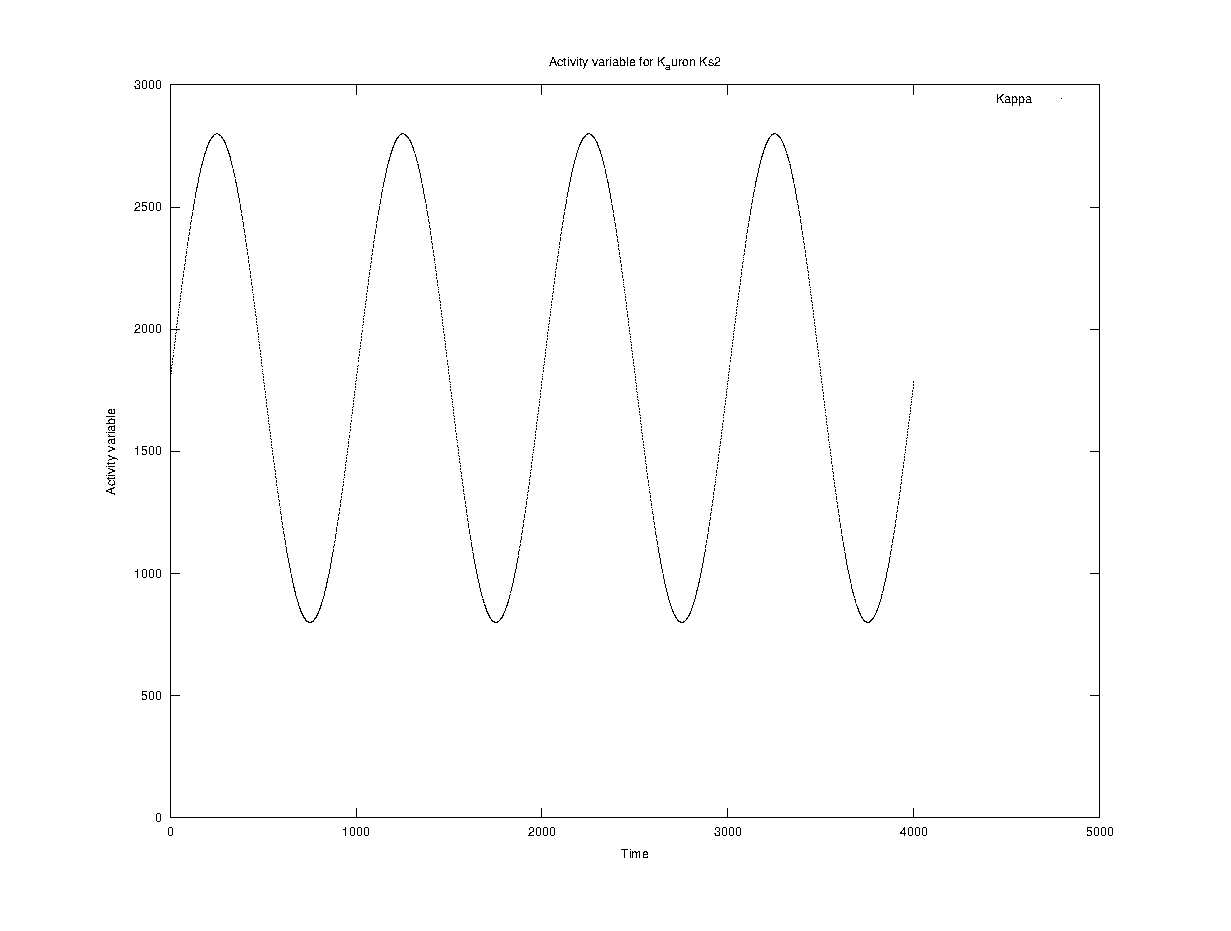
\includegraphics[width=0.5\textwidth]{./synapticTransmissionPlots/eps_auronKs2-kappa.eps} 		} 
   	\subfloat[Synaptic transmission]{\label{figSynTransmission:edge-b} 		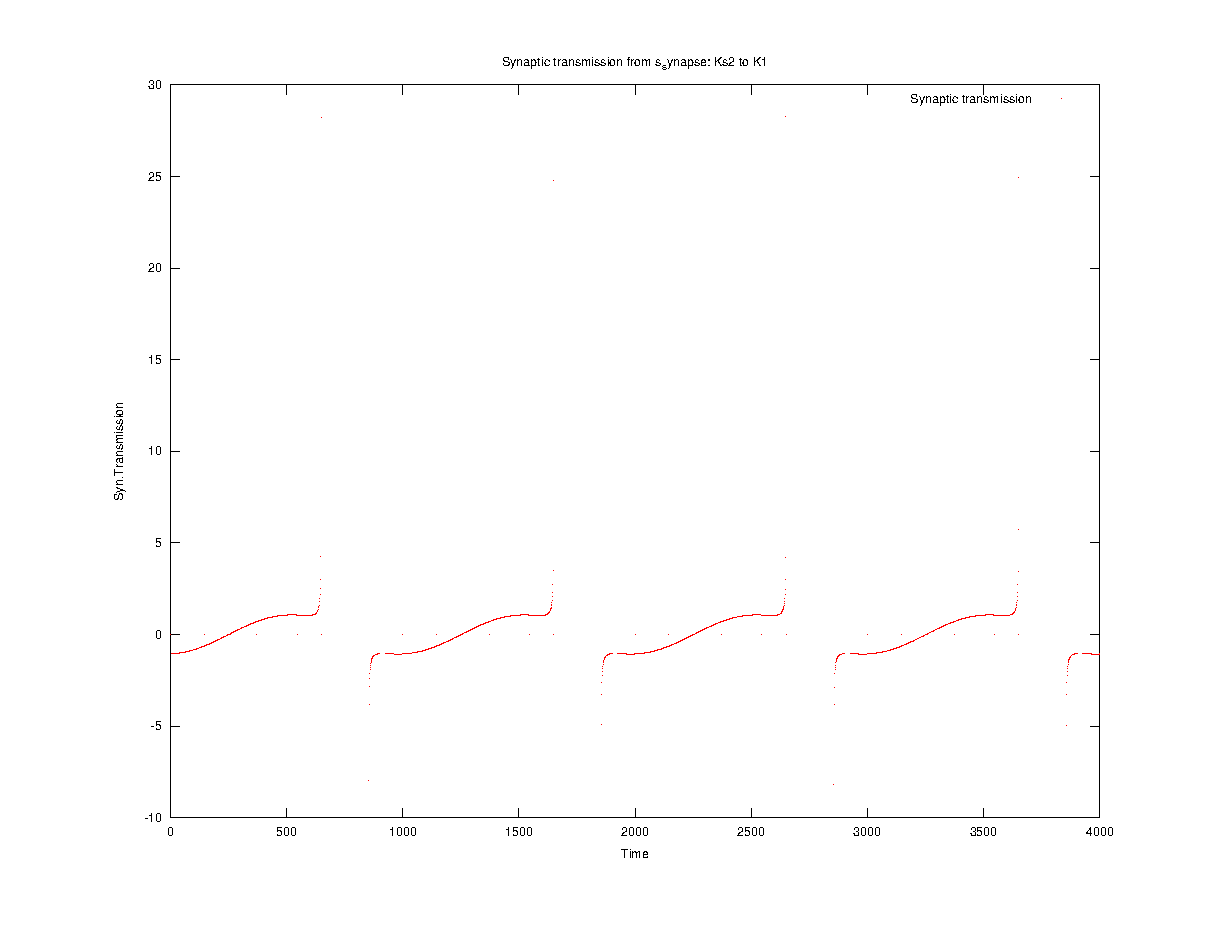
\includegraphics[width=0.5\textwidth]{./synapticTransmissionPlots/eps_transmission_Ks2->K1.eps} 	}
	%\caption{Demonstration of the value function for changing kappa}
	\label{figSynTransmission}
	\caption{The presynapsic activity variable kappa ( \ref{figSynTransmission:edge-a}  ) and the following synaptic transmission ( \ref{figSynTransmission:edge-b} ). 
			Notice the nonlinearity of the synaptic transmission when $\kappa_j \leq \tau$.}
\end{figure}


			When the presynaptic activity variable, $\kappa_j$ varies as a sin( t ) and is at all times above firing threshold, the synaptic transmission will wary as its derived, the cosine.
			%LEGG VED PLOT for [kappa alltid over terskel] også?
			If the presynaptic activity variable as times is equal or below the firing threshold, the plot becomes more interresting.
			Figure \ref{figSynTransmission} shows the presynaptic activity variable, $\kappa_j$ and the following transmission in the synapse. 
			The plots are made from the octave log files following one run of the implementation.

			When $\kappa_j$ approaches the threshold, the presynaptic period goes toward infinity. This causes a synaptic transmission $\kappa_{ij}$ of size zero.
			Since the edge transmission in the implementation is the derived of $\kappa_{ij}$, we get the nonlinearity when $\kappa$ goes below the firing threshold of the presynaptic neuron.
			In the empty interval in the synaptic transmission curve it can be seen that $\kappa_j$ is below the $\tau$, and we do not need to have synaptic transmission.
			% Skrive at dette er ordna med ei if-setning?


		%\subsection{Skrive om implementasjon av dette}
		%\subsection{Skrive om effekter ved denne metoden}
		%	\begin{itemize}
		%		\item At når $\kappa$ nermer seg $\tau$, vil perioden gå mot uendelig veldig raskt. For diskret system vil dette oppfattes som en ulinearitet 
		%		(peride går fra normal verdi til veldig høg verdi -> overføring går "plutselig" til 0). Dette fører til en høg derivert som sørger for at $W_{ij}=0$. Vis transmission plot.
		%		\item at når vi velger å integrere opp den deriverte (overføring) for å finne state, vil vi får 'integral--error' for $\kappa_{post}$.
		%		Dette fører til neste avsnitt: "rekalkulering av Kappa".
		%	\end{itemize}


		\subsection{Relcalculating $\kappa$}
		\label{ssecRecalcKappa}
		Because synaptic transmission is implemented as the derived of the $\kappa_{ij}$, and the postsynaptic activity variable $\kappa_i$ as the integral of this kind of synaptic transmission
		, we have to consider the trunction error of $\kappa_i$. 
		Every small error in the calculated $\kappa_i$ will for ever be a part of the result, and we can get potential large errors after a relatively short time.

		For this reason it is important to recalculate $\kappa_i$ periodically.
		For the recalculation of $\kappa$, a period with the right balance between recalculating to often and not often enough was devised.
		If the recalculation happens to often, to much effort will go into recalculating $\kappa$, and if the recaluclation happens to seldom, a global trunction error of unacceptable size might emerge.

		The truncation error might vary with variables such as hardware architecture, system load and even the individual auron's activity level,
		Because it is hard to know the level of the individual auron's truncation error, the period between recalulation of truncation error is designed to be adaptive as a function of the last error.
	%	The time of the next recalculation of the auron's $\kappa$ is computed after $\kappa$ is recalculated, as a function of the error given from the present recalculation.

		%To best achieve this, the period between recalculating $\kappa$ is designed to be dynamic as a function of the error at the last recalcualation. 
		It is important to limit both the minimum and the maximum period between recalulations of $\kappa$.
		To achieve this, an altered sigmoid function has been devised for this purpose.
		This function should have the maximum value when the error is zero ($\lim_{E \to 0} p_e(E) \neq \infty$) and a minimal period ($\lim_{E\to\infty} p_e(E) \neq 0$).
		This function should therefore have a maximum when the error is very small, and a minimum period as the error grows very large. 
		%OVER: XXX Dårlig skrevet (bare siste linja)

		An altered sigmoid function suitable for this purpose has been devised.
		%I have devised an altered sigmoid function suitable for this purpose.
		\begin{equation}
			\label{eqAlteredSigmoidFunk}
			p_e(E) = (c_1+c_2) - \frac{c_2}{1+e^{-(c_4*E-c_3)}}
		\end{equation}


		\begin{figure}[bht!]
			\begin{center}
				\includegraphics[width=0.95\textwidth]{sigmaPlot.eps}
				%\caption{Demonstration of the value function for changing kappa}
			\end{center}
			\caption{Plot of the altered sigmoid function (eq. \ref{eqAlteredSigmoidFunk}), with \mbox{$c_1$ = 100}, \mbox{$c_2$ = 250}, \mbox{$c_3$ = 10} and \mbox{$c_4$ = 0.5} }
			\label{figAlteredSigmoidFunction}
		\end{figure}
	
		This will give a the largest output value when the error is very small. For increasing errors, the output of the altered sigmoid function will become smaller.
		We can see from plot \ref{figAlteredSigmoidFunction} that the altered sigmoid function \eqref{eqAlteredSigmoidFunk} give a maximal and a minimal period for the recalculation of $\kappa$.
	
		From \eqref{eqAlteredSigmoidFunk} we can see that the altered sigmoid function has the maximum value of $c_1+c_2$.
		In fig. \ref{figAlteredSigmoidFunction} the values $c_1 = 100$ and  $c_2 = 250$, giving the maximum value as 350 time iterations between recalculation of $\kappa$.
		Because of a small degree of truncation error in the small test cases used while testing this implementation, the minimal period between recalculation was set so $c_1=100$ time iterations. 
		This can easily be altered for larger test cases, or other situations where the truncation errors become an issue.
		% TODO Skriv om det under. Blir overflødig..
		%The altered sigmoid function \eqref{eqAlteredSigmoidFunk} is used when the period to the next recalculation of $\kappa$ is planned. 
		%The maximum value, in this context, gives the maximum period before the new recalculation is done. %This happens when the error is wery small (se fig \ref{figAlteredSigmoidFunction}).
		%The minimal and maximal period between recaluclation can be modified by altering the constants $c_1$ and $c_2$.

		%TODO skriv litt om, de neste to avsnitta.
		% TODO SKRIV DETTE, MEN SKRIV OM FØRST :  One other thing that is worth noting is the variables $c_3$ and $c_4$ giving the shape of the curve. $c_4$ gives the lenght of the curve, that is how steep it is.
		


		% TODO TODO TODO TODO TODO TODO TODO TODO TODO TODO TODO TODO TODO TODO TODO TODO TODO TODO TODO TODO TODO TODO TODO TODO TODO TODO TODO TODO TODO TODO TODO TODO TODO 
		% Har rudda i tekst til hit.
		\subsection{------------ Har rydda i tekst, til hit ------------- }

		After some analysis, I desided to use the values used in fig. \ref{figAlteredSigmoidFunction}.
		This gives a function that gives maximum period between recalculation of $\kappa$ when the error is below about 10. 
		It has a relatively steep decent between an error of 10 and 30. The minimum period is set to 100 time steps and the maximum to 350 time iterations.

		The minimum time between recalculation of $\kappa$ will limit the use of resources. %cause the simulation not to use to much resouces.
		The maximum value of this function is limited because the error will have a stocastic nature, and one could e.g. end up with zero error if one get equal positive and negative errors.
		This could potentially give a very large period before the next recalculation of $\kappa$.

		Because of the stocastic element of the trunction error, the planning of the next recalculation of $\kappa$ is also implemented as a FIR--filter with a moving average over the last three values.
		%For this reason, the calculation of the period between recalculation of $\kappa$ is also implemented as a FIR--filter with a moving average over the last three values.
		%
		%When the auron is constructed, $\kappa$ is recalculated before any input synapses is defined. This gives the filter a small initial period.
		When the simulation starts, $\kappa$ is first calculated by the recaluclate function, giving the recalculate function a small initial period based on the level of synaptic input.
		% ELLER MEIR RETT: The first time $\kappa$ is calculated, it is calculated with the recalculate function, giving the filter a small initial period, based on the initial level of input.
		Aurons with a large initial input will therefore get a smaller initial recalculation period that some auron with a smaller initial input. %due to a large initial error.

		\subsection{Implementation of recalculation of $\kappa$}
		The execution of the planned recalculation of $\kappa$ is done in the same way as the execution of the planned action potential for the $\kappa$ auron.
		In the next section I will use some time on evaluating different methods for executing planned events at the planned time.
		The choice of method for this implementation is described in section \ref{ssChoiceOfTimeEstimationForThisImplementation}.
		
		For recalculation of $\kappa$ with the chosen method, we need a separate object whose doTask() function will call the K\_aurons recalculateKappa() function.
		To achieve this, each K\_auron has its own object of the class recalcKappaClass().

		recalcKappaClass::doTask() then will call the associated K\_aurons recalculateKappa() function, in addition to planning the time of the next recalculation according to the considerations in section \ref{ssecRecalcKappa}.
		

% HER EHER HER er eg.

		%Siden kappa bare regnes ut som integralet av den deriverte, vil det være behov for rekalkulering av Kappa, i ny og ne. Dette bør ikkje skje for ofte, heller ikkje for sjeldent.
		%Difor: lage en adaptiv utførelse av dette. Dette sjekker avviket mellom den rekalkulerte verdien og den gjeldende verdien, ved rekalkulering. 
		%
		%Dette avviket sjekkes opp i mot en predefinert ønska verdi, og differansen er med på å bestemme om periode til neste rekalkulering skal auke eller minke (auker/minker som en funksjon av avvik-avviket). 
		%
		%Dette avviket er m.a.o. med på å bestemme tid til neste rekalkulering av Kappa.
		%Auken/minken bør ha en maksverdi.




	\section{Estimation of firing time}
	For KANN, synaptic transmission can be defined as transmission of change in the postsynaptic node's input level.
	The input of a node, in terms of $\kappa$, is propotional to the synaptic weight and inversly propotional with the presynaptic inter--spike period.

	When the presynaptic node changes its activation level, and its period increases or decreases, the level of synaptic transmission will be altered accordingly. 
	Because of the number of synapses per axon/ dendrite, it is most efficient to perform as many of the calucations as possible in the presynaptic auron.
	For this reason, the most efficient way of calucating the postsynaptic dendrite's activation level is to let the synapse transmit the derived of the signal (change).
	%TODO Har skrevet dette tidligare. (to subsections før). Skriv om, og referer/underbygg denne måten.

	If the transmitted varible is the derived of the signal the postsynaptic dendrite can easily calculate the changed postsynaptic $\kappa_i$, as sen in section \ref{ssecSynInputToANode}.
	% XXX SAGT FØR: If we define $\kappa_{ij}$ as the contribution on $\kappa_i$ from the synapse between node $j$ and node $i$ , $\kappa_i$ can be calculated as
	%\begin{equation}
	%	\kappa_{i} = \sum_j{\kappa_{ij}}
	%\end{equation}
	
	If every $\kappa_{ij}$ but one, $\kappa_{ix}$, is kept constant, it can be shown that $\Delta \kappa_i$ is equal to $\Delta \kappa_{ix}$.
	Following that $\kappa$ is calculated as a superposition of all the input synapses contribution, these equations can be extended to change of transmission of multiple synapses.
	This gives us the equation for the change of postsynaptic activation level following synaptic transmission at synapse from node $x$ to node $i$.

	\begin{equation}
		\kappa_{ij, new} = \kappa_{ij, old} + \Delta \kappa_{ij}
	\end{equation}

	Instead of calculating all of this at every synapse, or for every synapse at the postsynaptic dendrite, it is better to calculate as much as possible presynapticlly.
	This gives one calulation every time a node fires an action potential, instead of one for every output synapse.

	%XXX XXX XXX Trur eg skrive  resten i subsubsection: implementation:KANN -> pEstimatedTaskTime -> execution of elements
	
	% TODO SKRIV litt om dette her, og lag eit frampeik til etter pEstimatedTaskTime, der eg skal skrive meir om dette.
	%Transmission of the derived solves many problems concerning efficiency, but it also introduces integral error for the postsynaptic $\kappa_i$
	%This problem can be solved, and we will come out JAJAJ. Skriv anna gang-- TODO


	%Etterkvart: skriv om integral-errors og fiksing av dette ved å bruke pEstimatedTaskTime (regelmessig fiksing, som er adaptiv med basis i feilen på postsyn signal (høg feil=>oftere regelmessighet på resumming av kappa)).


	When the firing time is estimated, it is fundamental that we have a mechanism for executing these elements at the right time. 
	In the following sections i propose two different solutions for this. 
	In section \ref{ssChoiceOfTimeEstimationForThisImplementation} the choice for this implementation will be presented, and different pros and cons with each method will be discussed.



	
	\subsection{pEstimatedTaskTime}
	$\kappa$ANN is based on calculating the firing time, given the present level of input. 
	Because the input level of an ANN node varies constantly, the calculated firing time is but an estimation of the nodes firing time. 
	The estimation of the nodes firing time changes as the input level does.
	%The estimated firing time for a node changes as the input level does.
	
	The std::list pEstimatedTaskTime is basically an array of dynamic size consisting of std::list--elements,
	where the outer list is an array of future time iterations and the inner lists are arrays of tasks estimated for the respective future time iterations.
	%The inner list is an array of tasks, the outer list is an array of future time iterations. 
	%This can be used for planning the time of execution for different tasks.
	%that keeps overview of when the tasks in the inner tasklist is to be executed.

	The outer list could be said to be the time iteration (relative to the present time iteration) when the tasks in the conlaining list are to be performed. 
	When every task in the inner task list is completed, % ELLER "moved to the pWorkTaskQue" 
		the task list is removed from the outer list. 
	In this way it is possible to keep the relative time--task list updated.

	The tasks located in the inner list of the first element of the outer list are the tasks that are to be executed the next time iteration.
%	Tasks that are to be performed the next time iteration is inserted in the first element (inner list) of the outer list.
%	In time\_class::doTask(), the first element of the outer list (the first inner list) is evaluated, and all the taskt are executed. 
	time\_class::doTask() is responsible for tasks being executed at the planned time. 
	Before time\_class::doTask() iterates time (and moves its pointer from the first element to the last element of pWorkTaskQue), all tasks that are planned for next time iteration is moved from pEstimatedTaskTime to pWorkTaskQue.
	The tasks are appended at the back of pWorkTaskQue before the time\_class object pointer is moved to the end of pWorkTaskQue. 
	This will cause the planned tasks to be performed the next time iteration.

%	Before the discrete time is iterated, the first element is removed from the outer pEstimatedTaskTime--list.
%	In this way it is possible to keep an overview of the immediate future with pEstimatedTaskTime.

	If a new element (a new task) is to be inserted somewhere outside the present scope of the pEstimatedTaskTime, the element (std::list) needs to be constructed.
	Because of the mechanisms of pEstimatedTaskTime, not only the element needs to be produced but also all the estimated time iterations between the length of pEstimatedTaskTime and the estimated time of the respective task.

%dette står lenger nede, under "insertion of elements"
%\begin{lstlisting}
%int nDiff = uRelativeTime - pEstimatedTaskTime.size();
%if( nDiff >= 0 ) //Mangler ledd. Legg til rett antall.
%{
%  for(int i=0; i <= nDiff; i++){
%  pEstimatedTaskTime.push_back( new std::list<timeInterface*> );
%  }
%}
%\end{lstlisting}
	
	\subsubsection{Insertion of elements}
	The std::list container is implemented as a doubly linked list\cite{Stroustrup2000KAP16}.
	To find element nr. $n$ we can iterate throught the list $n$ times from the beginning.
% 	To find element nr. $n$ we can either iterated throught the list ($n$ times) from the beginning, or $S-n$ iterations from the end.
%	An alternative approach if we are concerned with efficiancy, is to iterate from the end that is closest to the element (the beginning or the end of the list).
	In doubly linked lists, we can also iterate thourgh the list from the end.
	If we always iterate from the end that is closest to the target element, the number of iterations required will be halved (if the target position is completely random within a fixed--size list).

	If, for example, we have a list that is 10 elements long and want to access element nr. 9, the most efficient way of doing this in a doubly linked list is to start at the end.
	To generalize this, we can say that if the element that needs to be accessed is later than $\frac{[\text{size of list}]}{2}$ the ``search'' will start at the end.

\begin{lstlisting}
if( uRelativeTime_arg < (pEstimatedTaskTime.size())/2 ){
  // Seach from the last element.
}else{
  // Seach from the first element.
}
\end{lstlisting}

	%If, however, the estimated task time is outside the scope of pEstimatedTaskTime, new elements will have to be inserted.
	Insertion of tasks outside the immediate length of pEstimatedTaskTime requires some attention.
	When an event is planned for some time iteration outside the scope of pEstimatedTaskTime, the scope of pEstimatedTaskTime will have to be increased.
	Because the pEstimatedTaskTime works as a FIFO--que, where the first element % (containing a list of all the planned tasks for the future time iteration)  (se section \ref{ssecEvaluationOfpEstimatedTaskTimeELEMENTS})
		is popped in time\_class::doTask(), it is important to insert every element between the present scope of pEstimatedTaskTime and the new planned task time.
	This is done by
\begin{lstlisting}
int nDiff = uTimeToTask-pEstimatedTaskTime.size();
if( nDiff >= 0){
  for(int i=0; i<=nDiff; i++)
    pEstimatedTaskTime.push_back( new std::list<timeInterface*> );
}
\end{lstlisting}
%This algorithm enshures that pEstimatedTaskTime is correct in terms of time planning.
The expression in the for loop is the reason for having the outer elements of pEstimatedTaskTime defined as std::list$<$timeInterface*$>$ pointers.
In the above algorithm, new std::lists are created in the free store. This creates elements for pEstimatedTaskTime that will exist after the return from the function where the elements are constructed.
%When the free store is used, it is important to deallocate the memory after the element is used. %skriv bedre, denne setininga
To avoid memory exhaustion, it is important to deallocate the memory allocated in the free store when the variable no longer will be used. This is done when the inner lists are evaluated in \emph{time\_class::doTask()}.
For more about the execution of pEstimatedTaskTime tasks, se section \ref{ssecEvaluationOfpEstimatedTaskTimeELEMENTS}.
%TODO Skrim om deallocating memory i ssecEvaluationOfpEstimatedTaskTimeELEMENTS   asd123


	%TODO Koden for denne insertion--funksjonen skal være med i appendix!
	% 			- og skal refereres til fra [her]



%
% 	Skriv om at funk får inn relativ tidsflytt som argument. For å finne relativ tidsflytt trenger eg å lagre gammelTidsPkt i timeInterface-objekt.
% 	Skriv om iterator opplegg. Iterator-returnerende funksjon som søker seg fram til rett ytre-liste (fremtidig tidsiterasjon..)

	\subsubsection{Moving tasks in pEstimatedTaskTime}
	When the planned task time for a timeInterface object is changed, the pointer to the object have to be moved in the pEstimatedTaskTime list.
	
	%In the standard library containers, pointers to elements are called iterators. An iterator 

% TODO TODO TODO TODO TODO TODO TODO TODO TODO TODO TODO TODO TODO TODO TODO TODO
% TODO TODO TODO TODO TODO TODO TODO TODO TODO TODO TODO TODO TODO TODO TODO TOD
% TODO TODO TODO TODO TODO TODO TODO TODO TODO TODO TODO TODO TODO TODO TODO TO
% TODO TODO TODO TODO TODO TODO TODO TODO TODO TODO TODO TODO TODO TODO TODO T
	%TODO lagre heller iteratoren i timeInterface objektet. Tar langt mindre tid. Trur det at iteratoren blir invalidated bare gjelder for vector..
	XXX KORLEIS skal eg gjøre dette? No lagrer eg ulTid i objektet. Kanskje eg heller skal lagre list<list*>::iterator ? Funker dette bedre?
	\emph{Det er bare for vector at iteratoren blir ivalidated når størrelsen på container endre!}

	%Uavhengig av korleis eg finner element, kan eg skrive om flytting av element:
	When the estimated task time is altered, one can assume that the new position will be located not far from the old position, compared to the size of the whole pEstimatedTaskTime list.
	In this case, the most efficient way of finding the new position is to iterate $x$ positions from the old estimated time iteration in pEstimatedTaskTime, instead of finding the position from one of the ends of pEstimatedTaskTime.
	The relative moval of the task can be desided by taking the difference between the new estimate and the old estimate of the task time, $x$, and move the object pointer $x$ iterations along pEstimatedTaskTime. 
	$x$ may be positive or regative.
	
%	\subsubsection{Flytting av element}
%	Implementer først, så skriv om flytting av element som resultat av ny $\kappa$.
%	Element vil ikkje flyttes langt, så beste vil være å flytte elementet fra [no-posisjon].
%	Dette kan lett gjøres i ei `doubly linked list'.
%
%	(planen no er å flytte den ved å ta inn no-iterator-plass (som er lagra i K\_auron) og kor langt den skal flyttes. 
%	Dette gjøres best ved å overlagre funksjonen for når den får argument (iter, timeInterface, tidsFlytt). 
%	Bør returnere iterator, for at auronet skal ha muligheten til å lagre også ny iterator i pEstimatedTaskTime).




	\subsubsection{Evalutation of pEstimatedTaskTime elements}
	%\subsubsection{execution of element tasks}
	\label{ssecEvaluationOfpEstimatedTaskTimeELEMENTS}

	%pEstimatedTaskTime: where all planned tasks for future time iteration lies,
	%pWorkTaskQue: where the tasks for the immediate future lies.
	When the time iteration for the planned events in pEstimatedTaskTime arrives, the tasks in the pEstimatedTaskTime element need execution.

	This can be done by executing the tasks in a separate function, e.g. time\_class::doTask(), that is called at an ideal time for evaluating pEstimatedTaskTime elements.
	%time\_class::doTask() is ideal for executing the tasks. 
	To be consistent about the execution of tasks, it is better to move the tasks planned for the next time iteration from the next element in pEstimatedTaskTime to the pWorkTaskQue list.
	pWorkTaskQue is the list used to plan the immediate future for the ANN, initially developed for the SANN model that focus more on the immediate state of the system.

	When this is done in time\_class::doTask() before time is iterated and the time\_class time separation object is moved to the end of pWorkTaskQue, the tasks from pEstimatedTaskTime will be executed the next time iteration.
	%When the estimated time for the elements task is at the next time iteration, time\_class::doTask() will insert a pointer to the element into pWorkTaskQue.
	%This will will call the node elements \emph{doTask()} function the next time iteration. 

%	The elements of pEstimatedTaskTime is created in the free store, and needs to be deallocated to avoid memory exhaustion. 
	When a pointer to an element is removed from pEstimatedTaskTime, the elements destructor is not called. 
	%When an element is removed from pEstimatedTaskTime, the value of the dereferenced elements destructor is not called because the element is a pointer. 
	It is therefore important to deallocate the memory used for the object in the free store to avoid memory exhaustion.
	%When the element us used and no longer needs to be stored, 
	At the end of time\_class::doTask() this is done explicitly:
\begin{lstlisting}
delete pEstimatedTaskTime.front();
pEstimatedTaskTime.pop_front();
\end{lstlisting}
	The \emph{delete} operator frees the memory allocated to the task list planned for the next time iteration (the dereferenced pointer)
	and the \emph{pop\_front{}} operator removes the now empty pointer in the first element of \emph{pEstimatedTaskTime}.


	

% TODO Skrive eksempel med "the action potential cascade? :
	%I will in the remainder of this section focus on the action potential cascade. 
	%When the firing time of the auron is estimated, a pointer to the auron node element is inserted into pEstimatedTaskTime. 
	%When the time comes for the auron to fire an action potential, the auron pointer is interted into pWorkTaskQue, and the \emph{K\_auron::doTask()} will be executed at the estimated time iteration, inducing the action potential cascade.

	%For K\_aurons, the \emph{doTask()} will first calculate the aurons inverse period (``instantaneous frequency''). 
	%The result is variable \emph{K\_auron::uLastCalculatedPeriod} is made to save this value for later use.
	
	%The new period is calculated, using equation \eqref{eqPeriodeligningForKonstIntraPeriodKAPPA}, giving the level of transmission at the nodes output synapses.
	
	%skriv litt om at denne ligninga er basert på konst. interspike kappa. Dette har vi ikkje her. Kvifor er det viktig alikevel. 
	% 	- delay i ANN. Vente på første spike kan være uoptimalt, men det vil være proposjonalt med aktiviteten, som kan være bra. osv. Drøft (seinare, nevne det her..)
	% 	- arbeidsbelastning.
	

	%\subsection{Checking a member variable of timeInterface--derived elements}
	\subsection{Checking estimated task time directly from time\_class::doTask()}
	A more direct approach is to check the elements estimated firing time directly from time\_class::doTask(). 
	Every class derived from timeInterface contains a variable called ulEstimatedTaskTime where the elements estimated task time is written every time this is updated.
	If we check ulEstimatedTaskTime every time iteration, and number is the same as the next time iteration's index (ulTidsiterasjoner), time\_class::doTask() is responsible to insert its pointer into pWorkTaskQue.
	This will cause the element to do its task on the planned time iteration.
	%If lEstimatedTaskTime is the same as the next time iterations ulTidsiterasjoner, we can insert a pointer to the element into pWorkTaskQue, causing it to do its task next time iteration.

	When $\kappa$ is updated, and K\_auron::doCalculation() updates the aurons estimated firing time, it also updates the K\_auron::lEstimatedTaskTime.
	If $\kappa$ is less than the firing threshold, the K\_aurons lEstimatedTaskTime is set to 0. 

	\subsubsection{Execution of elements}
	time\_class::doTask() runs through the list K\_auron::allKappaAurons to see if any elements have an estimated firing time the next iteration.
	When it finds an element scheduled for the next iteration, the pointer to the element is imnserted into pWorkTaskQue.


	\subsection{Choice for this implementation}
	\ref{ssChoiceOfTimeEstimationForThisImplementation}
	% XXX TODO BEGRUNN GODT KVIFOR EG HAR SKREVET SÅ MYKJE OM pEstimatedTaskTime! Det holder ikkje at eg har gjordt det.
	% 	Skriv at det er godt mulig dette er den mest effektive algoritmen når antall noder auker kraftig!
	% 	Skriv at i såfall må en maks-lengde på lista lages.
	The two methods for execution of tasks at the planned time both have flaws and cons.
	
	pEstimatedTaskTime krever at alle flyttinger av element er riktig. Dersom det er mykje endring av kappa er dette dårlig for denne metoden (krever mykje flytting av element i pEstimatedTaskTime).
	Denne lista er derimot heilt uavhengig av antall auron vi simulerer. For store ANN vil nok denne pEstimatedTaskTime-varianten være best.

	Dersom vi har endring av kappa heile tida, kan metode 2 (den direkte metoden) være best.
	Da koster det ikkje noke å endre fyringsestimatet, men man har en konstant 'cost' ved iterasjon av tid. (BEMERK AT DENNE ER const SEINARE)
	Denne 'cost' er avhengig av antall K\_auron (da den må iterere gjennom alle element [med K>T?]). Denne 'cost' er constant for eit gitt antall auron.

	Det er to grunner til at eg har valt den siste metoden: 1) mine ANN vil være små med mykje endring av kappa. Dette gjør at det er heilt forsvarlig å velge metode nr. 1.
	Den andre grunnen til at eg velger metode nr.1 er at denne har konstant timedelay, noko som er bra..

	jeje... Osv.

	For this implementation, both methods were implemented and tested. 












\subsection{When do $\kappa$ propagate?}
Stavdal meiner at det er tull å propagere heile tida (kvar gang K oppdateres i presyn). 
Eg har laga plot for å sei imot dette: når kappa venter med å propagere til første fyring får man eit tidsdelay for depol til KN tilsvarende tida det tar til første fyring. (dette er veldig tydlig ved sprang i presyn K).

Når Kappa propagerer kvar gang presyn endres, fjærnes dette problemet. Propagerer som det er gjordt før, med at axon legges til i pWorkTaskQue. Alle postsyn. noder får dermed input tidligst neste iterasjon.

Dette har med synapstisk transmissjon å gjøre, og eg må gjøre dette ferdig før eg skrive meir om dette..

NEI faen! no er feilen der igjen. Sjekka kode, og fann at den propagerete, men bare om K>T, så det over er TULL.






%	\subsection{Anna fra tidligare:}
%	-- kanskje skrive om vanskene med log() ? Returnerer samme som argumentet, difor må vi typekonvertere til (float) eller (double) før man tar log() av det. Dette skapte hodebry, siden eg bare fekk resultatet 0.
% 		Ganga med FAKTOR, og fekk 0. Når eg typekonverterte argumenta til log() om til float gjekk fekk eg bra output..

%	Skriv også om at istedenfor å skrive $t_{estimert} = - \frac{1}{\alpha} \ln(\frac{\kappa-\tau}{\kappa-v_0})$ kan eg skrive $t_{estimert} = \frac{1}{\alpha} \ln(\frac{\kappa-v_0}{\kappa-\tau})$
%	(ferre operasjoner, meir effektivt!).

%	\subsection{simulering vha. ligning \eqref{eqVerdiligninga} fra section \ref{secMatematiskModelleringAvBioNeuron}}
%	\subsection{Osv.}












%antagligvis her, men veit ikkje heilt. Iterators. Brukes mykje, så bør forklares (spess for en C patriot)
%\subsection{Skriv om iterators, en plass}
%Dette er veldig viktig for produktet, så bør skrives om.
%
%Iterators er en høgare form for peiker. 
%I standard library er mange basisfunksjoner implementert, og små operatorer (som lenka liste iterering) er lett å implementere.
%Mange små funksjoner som er lett å implementere får alle en liten sannsynlighet for feil. Når det er mange av desse får man mange potensielle feil som er vanskelig å finne.
%
%I standard library er blandt anna en del "containers", som list. Dette er ei ``doubly linked list''.
%Man har også såkalla ``iterators'', som er en peiker til element i slike containers.
%Desse har blandt anna implementert iterator operatoren \emph{++}. Denne er garantert feilfri, og bør brukes fremfor å imlementere slikt selv (seier stroustrup)[referere!].
%
%Skriv at i tillegg til at man kan gå ut  fra at de er feilfri, så er de også godt optimalisert, og vil ofte gi en meir effektiv implementsjon.
%
%Iteratoren har veldig masse til felles med en peiker, bare med lettere, feilfri, meir optimalisert utførelse.


%\subsubsection{Ikkje mulig å lagre iteratoren}
%ELLER ER DET MULIG? (Kan være det under bare gjelder for vector!)
%
%Iteratore blir ugyldige, og gir udefinert oppførsel dersom lista blir rezised i mellom iteratoren blir laget og brukt. 
%Initiellt var tanken at K\_auron (og kanskje andre timeInterface som bruker pEstimatedTaskTime) skulle også inneholde en iterator (peiker) til rett element i lista.
%Siden iteratore blir ugyldig når listas lengde endres %stroustrup s. 550, nede. Understreka.
%	så går ikkje dette.
%
%Dette er grunnen til at kvar gang eit element skal flyttes, må det søkes opp på nytt (forrige plass kan inneholde eit nytt element, eller være forbi slutten av lista..)
%
%Siden vi ikkje bør anta kor den er, bør lista itereres gjennom på nytt. 
%En antagelse som er trygg er at elementet ikkje har flyttet seg veldig langt, når estimatet oppdateres.
%Dette gjør at det antagelig ligger i samme halvdel av lista, og det kan være lurt å begynne søket fra den siden som er nærmast ny plassering. %type før eller etter size() / 2 , før => start søk fra starten ...
%
%For å effektivisere, lages to funksjoner: en som legger til element, og en som flytter det. 
%Ved fyring av K\_auron fjærnes elementet, men skal også legges til på tidspkt. [no]+[estimert periode].
%Løsninga mi blir: i funksjonen som fjærner elementet, vil også nytt element legges til om element->periode. Dette er en rein insertion.
%
%For flytting av element må lista itereres gjennom, og kvar iterasjon må lista--elementet gjennomsøkes etter gjeldende element. 
%Dette er meir tidkrevende, og er grunnen til at eg skiller mellom de to operasjonene: insertion og moving of an element.
%
%Les stroustrup s. 550 for meir, når dette skal skrives om!












%*********************** Forenklinger *******************
\chapter{ANN simplifications and what is known in neuroscience}
Veit ikkje kor denne skal ligge, men
HER skal tabellen ligge. Diskutere korleis mine ANN er laga, kva forenklinger har eg gjort, og kvifor. (sjå side 27 i FDP-loggbok)

Referer en del til kapittel \ref{chapNeuroscience}.

Her skal eg legge inn tekst som impliserer at eg er reflektert. Skrive alle feil og mangler som ligger i mine modeller, og implementasjon-design.



%METODE for SAMMENLIGNING

\chapter{Comparison and result} %Dårlig kapittelnavn.


\section{Testoppsett for sammenligning av KANN og SANN}
	\subsection{Fleire testoppsett? Beskriv de ulike oppsetta, og kvifor!}
	\subsection{Teste for oppdelte nett: med koblinger med lite overføring/endring i overføring}


\section{resultat av sammenligning: SANN vs. $\kappa$ANN}


%Kanskje eg skal ha med "table of abbrevations" i appendix, eller først.

\bibliography{bibliografi}
%\bibliographystyle{abbrvnat}
\bibliographystyle{plain}
\end{document}

